

Jet-track correlation studies can produce measurements of the density of particles (in each $p_{\rm T}^{\rm trk}$ class) with respect to the jet axis and can also, by creating correlations weighted per-track by its $p_{\rm T}^{\rm trk}$, produce measurements of the distribution of $p_{\rm T}^{\rm trk}$ in the event as a whole.  Both types of measurements are presented here, for inclusive selections of jets with $p_{\rm T} > 120$ GeV at 2.76 TeV and 5.02 TeV, and for high-$p_{\rm T}$ dijet events at 2.76 TeV.  First, particle density correlation results are presented in Secs.~\ref{sec:inc_corr}-~\ref{sec:dijet_corr}.  Next, $p_{\rm T}^{\rm trk}$ distributions are used to extract measurements of jet shapes (the transverse momentum profiles of jets) in Sec.~\ref{sec:jet_shapes}.  Finally, in Sec.~\ref{sec:dijet_mpt}, $p_{\rm T}^{\rm trk}$ distributions are used to decompose and analyze the hemisphere momentum balance in dijet events.

\subsection{Inclusive jet particle density correlation results}
\label{sec:inc_corr}


Particle density correlation studies allow for the detailed characterization of jet fragmentation, and of medium-induced modifications to jet fragmentation in PbPb data (as a function of collision centrality) compared to pp data.  The analysis procedure described in Sec.~\ref{sec:JetTrack} results in fully-corrected 2D jet peaks in $\Delta\eta-\Delta\phi$, which may then be projected to obtain the distribution of particles in each $p_{\rm T}^{\rm trk}$ class as a function of $\Delta\eta$ or $\Delta\phi$.  The top panels of Figs.~\ref{fig:Inclusive_dEta1}-\ref{fig:Inclusive_dPhi4} show these $\Delta\eta$ and $\Delta\phi$ distributions (projected over $|\Delta\phi| < 1$ and $|\Delta\eta| < 1$, respectively) for 2.76 TeV pp data and PbPb data in each $p_{\rm T}^{\rm trk}$ range from 1--2 GeV (Fig.~\ref{fig:Inclusive_dEta1}-\ref{fig:Inclusive_dPhi1}) up to 4--8 GeV (Fig.~\ref{fig:Inclusive_dEta4}-\ref{fig:Inclusive_dPhi4}).  The bottom panels of these figures show the differences PbPb--pp for illustration of medium modifications to jet fragmentation patterns.  In both the $\Delta\eta$ and $\Delta\phi$ dimensions, centrality-dependent excesses of soft (low-$p_{\rm T}^{\rm trk}$) particles are evident.  These exhibit the greatest modifications in the most central PbPb collisions, decreasing with centrality until the most peripheral collisions show little modification when compared to pp data.  These excesses decrease with increasing $p_{\rm T}^{\rm trk}$, until in the 4-8 GeV range the enhancements evident at lowest-$p_{\rm T}^{\rm trk}$ reverse to possible slight depletion.  In both $\Delta\eta$ and $\Delta\phi$ dimensions, the soft excesses exhibit a gaussian-like distribution around the jet axis, while also extending to large angles $\Delta\eta = 1$ and $\Delta\phi = 1$ at lowest $p_{\rm T}^{\rm trk}$.  

Figures~\ref{fig:yield_deta_stacked} and~\ref{fig:yield_dphi_stacked} show the corresponding $\Delta\eta$ and $\Delta\phi$ distributions at 5.02 TeV.  Here, the distribution of particles in each $p_{\rm T}^{\rm trk}$ class are stacked (with lowest-$p_{\rm T}^{\rm trk}$ particles on top), and pp data shown separately at left.  Again the differences PbPb--pp are shown in bottom panels to illustrate the medium modifications, and exhibit similar qualitative trends to those described above for 2.76 TeV results.  Results may also be presented as a function of radial distance from the jet axis $\protect\Delta r = \sqrt{\Delta\eta^{2}+\Delta\phi^{2}}$.  Figure~\ref{fig:yield_dr_stacked} presents charged particle yields, differentially in $p_{\rm T}^{\rm trk}$, as a function of $\protect\Delta r$.  For comparison, the bottom row of each plot shows the difference, PbPb minus pp.  This shows the particles contributing to a jet fragmentation function measurement within a given radius from a jet, and illustrates the radial dependence of modifications extending to at least $\protect\Delta r = 1$.  


\begin{figure}[hbt] 
\begin{center} 
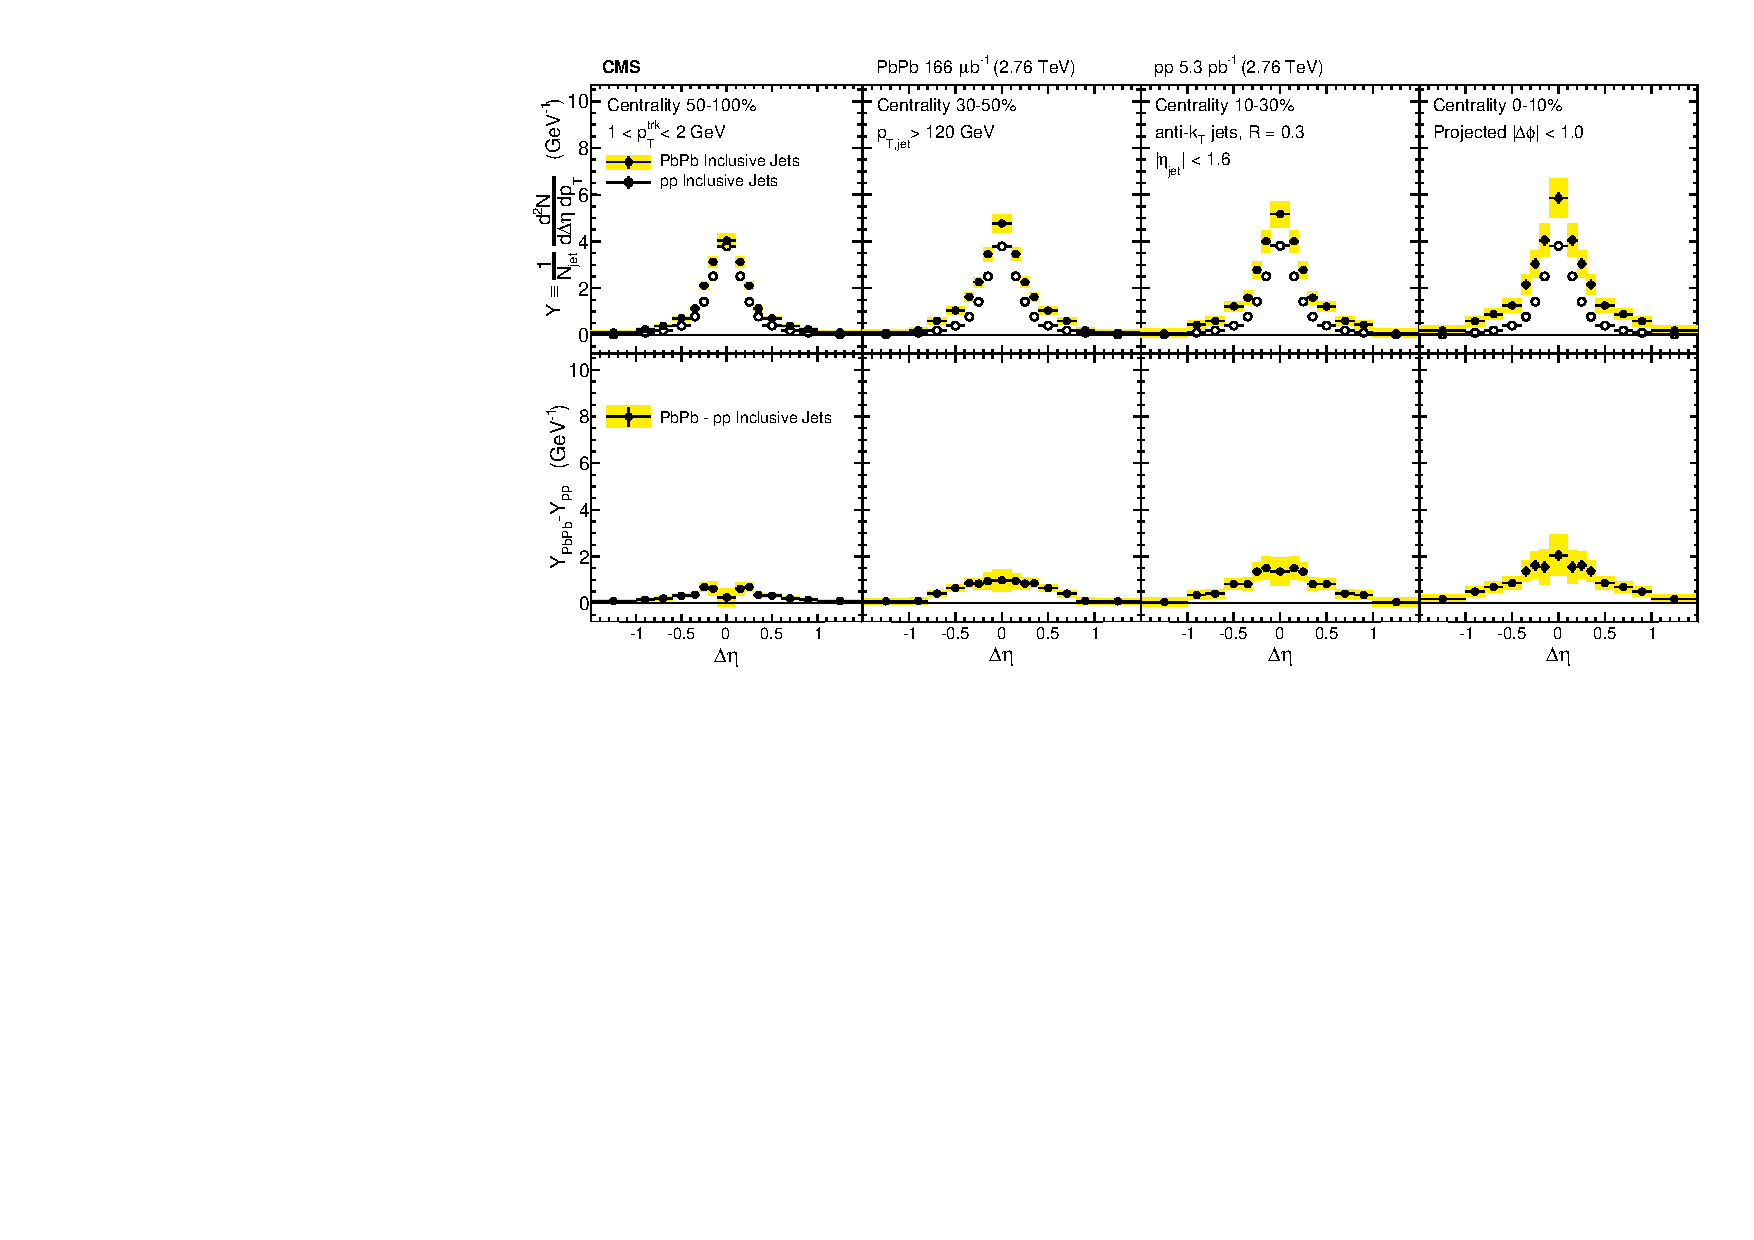
\includegraphics[width=0.99\textwidth]{figures/Results/PAS_Figure_3_TrkPt1_TrkPt2.pdf}
\caption[Inclusive jet $\Delta\eta$ correlations for tracks with $1 < p_{\rm T}^{\rm trk} < 2$ GeV at 2.76 TeV]{Symmetrized $\protect\Delta\eta$ distributions (projected over $|\Delta\phi| < 1$) of background-subtracted particle yields correlated to PbPb and pp inclusive jets with $p_{\rm T}>$ 120 GeV are shown in the top panels for tracks with 1 $ < p_{\rm T}^{\rm trk} < $ 2 GeV.  The difference in PbPb and pp per-jet yields is shown in the bottom panels. The total systematic uncertainties are shown as shaded boxes, and statistical uncertainties are shown as vertical bars (often smaller than the symbol size).}
\label{fig:Inclusive_dEta1}
\end{center} 
\end{figure} 

\begin{figure}[hbt] 
\begin{center} 
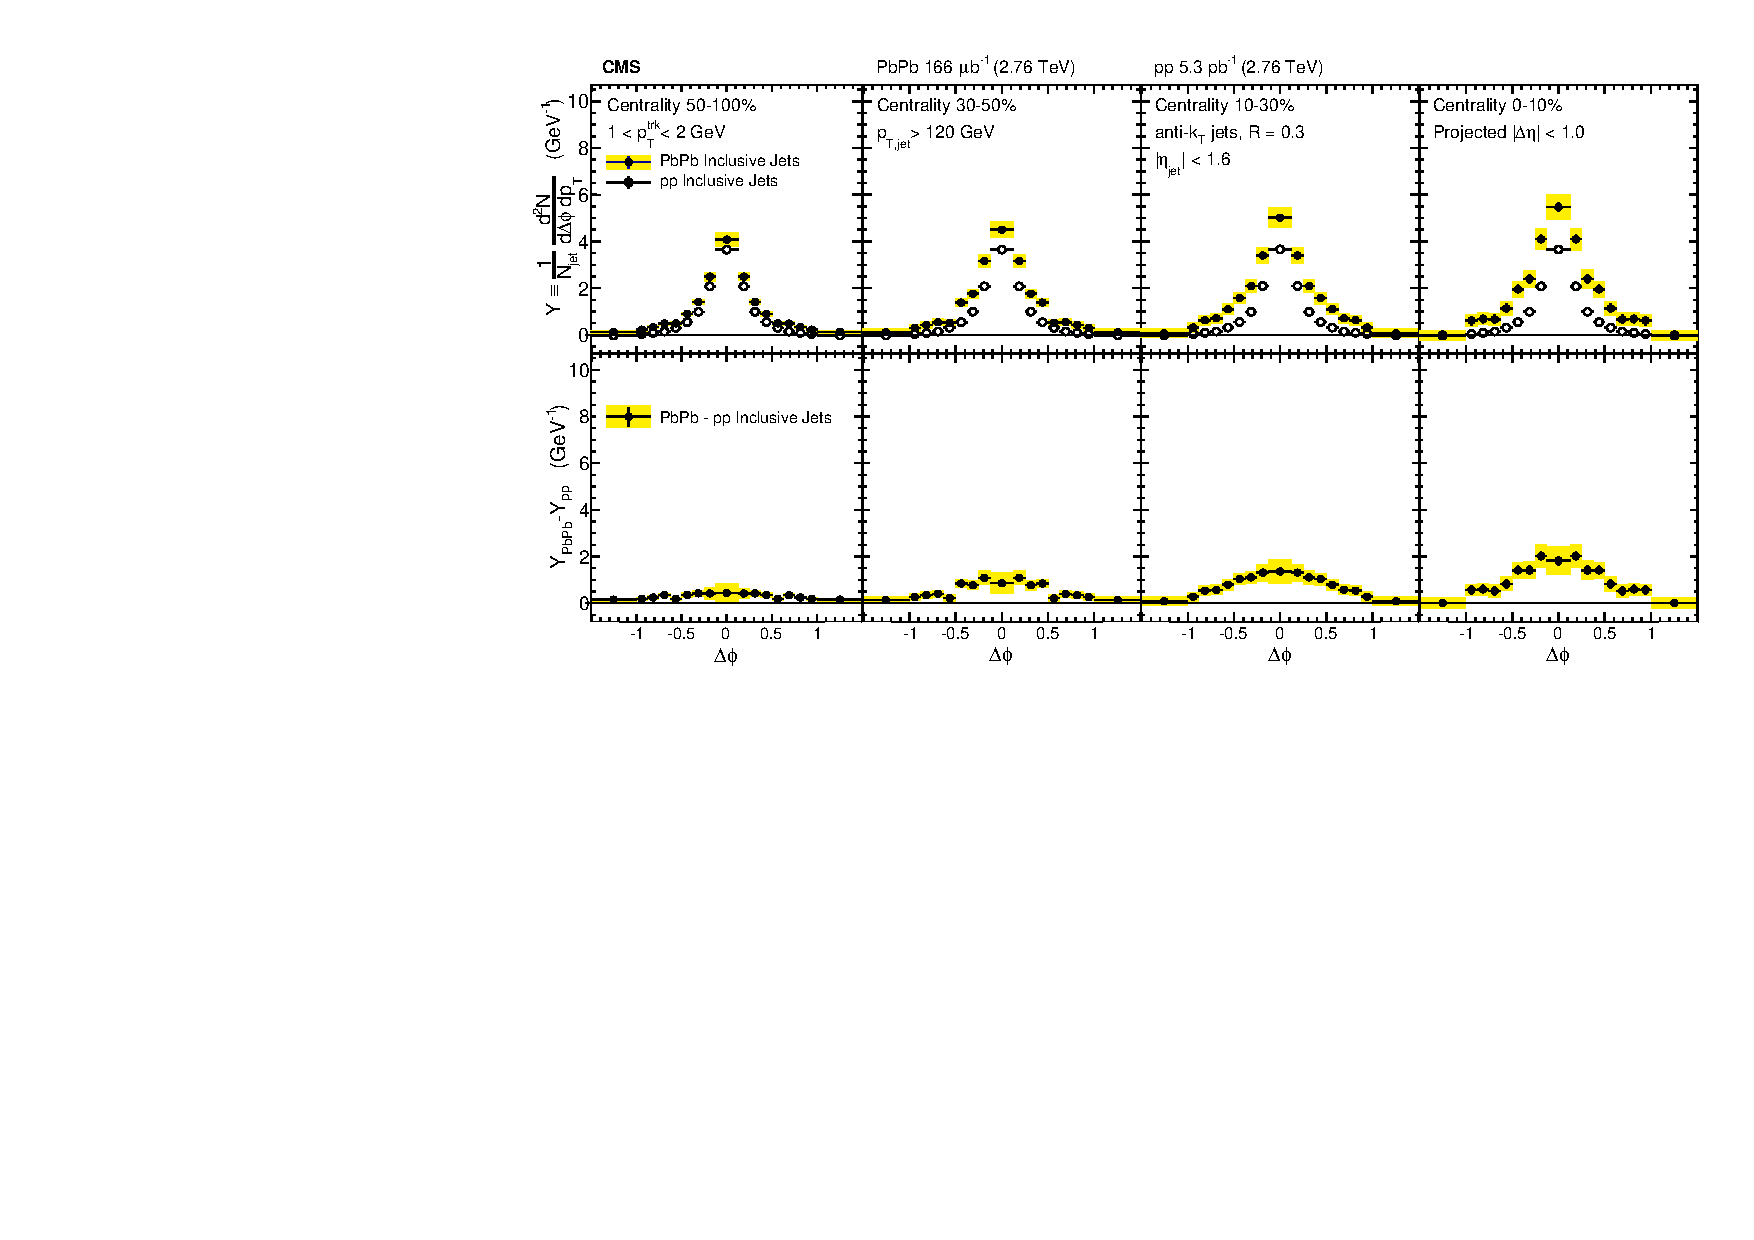
\includegraphics[width=0.99\textwidth]{figures/Results/PAS_Figure_4_TrkPt1_TrkPt2.pdf}
\caption[Inclusive jet $\Delta\phi$ correlations for tracks with $1 < p_{\rm T}^{\rm trk} < 2$ GeV at 2.76 TeV]{Symmetrized $\protect\Delta\phi$ distributions  (projected over $|\Delta\eta| < 1$) of background-subtracted particle yields correlated to PbPb and pp inclusive jets with $p_{\rm T} >$ 120 GeV are shown in the top panels for tracks with 1 $ < p_{\rm T}^{\rm trk} < $ 2 GeV.  The difference in PbPb and pp per-jet yields is shown in the bottom panels. The total systematic uncertainties are shown as shaded boxes, and statistical uncertainties are shown as vertical bars (often smaller than the symbol size).}
\label{fig:Inclusive_dPhi1} 
\end{center} 
\end{figure} 



\begin{figure}[hbt] 
\begin{center} 
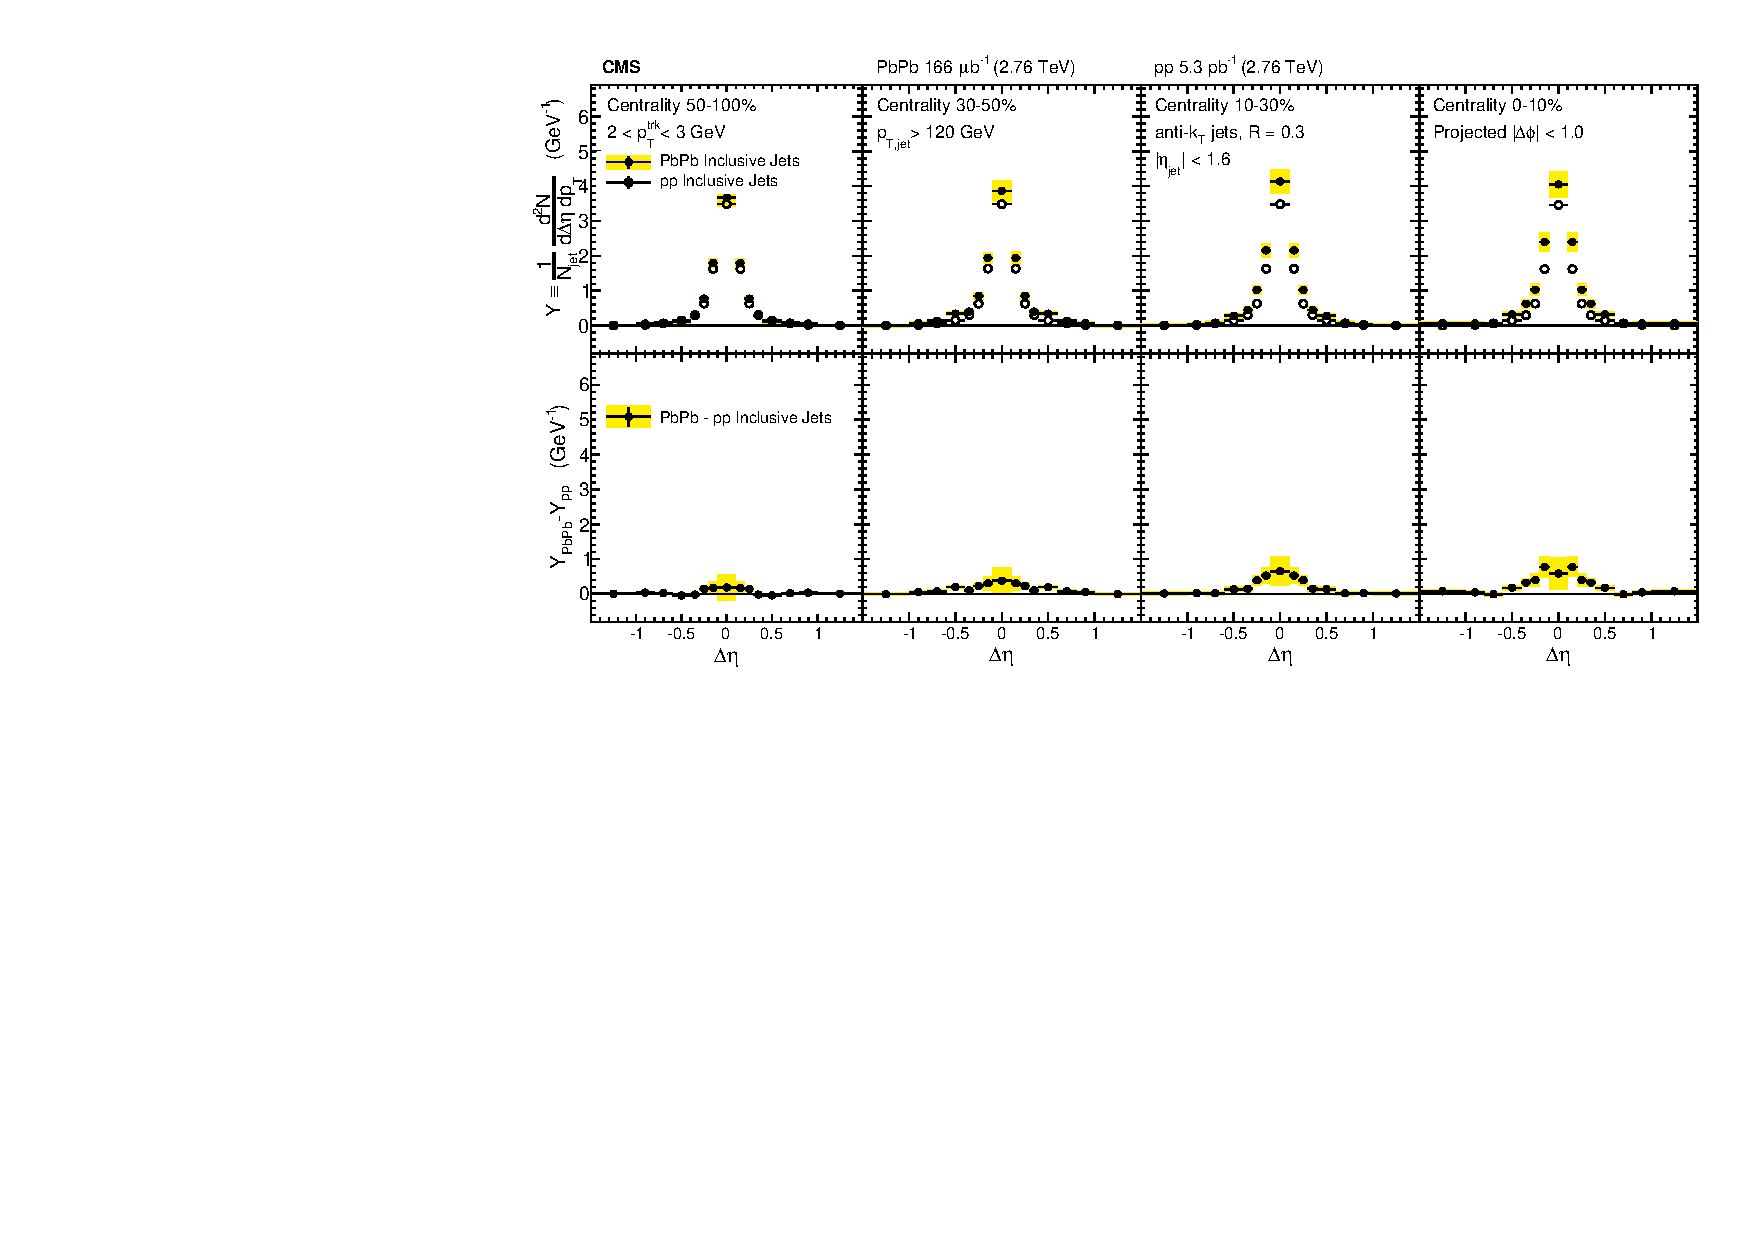
\includegraphics[width=0.99\textwidth]{figures/Results/PAS_Figure_3_TrkPt2_TrkPt3.pdf}
\caption[Inclusive jet $\Delta\eta$ correlations for tracks with $2 < p_{\rm T}^{\rm trk} < 3$ GeV at 2.76 TeV]{Symmetrized $\protect\Delta\eta$ distributions (projected over $|\Delta\phi| < 1$) of background-subtracted particle yields correlated to PbPb and pp inclusive jets with $p_{\rm T}>$ 120 GeV are shown in the top panels for tracks with 2 $ < p_{\rm T}^{\rm trk} < $ 3 GeV.  The difference in PbPb and pp per-jet yields is shown in the bottom panels. The total systematic uncertainties are shown as shaded boxes, and statistical uncertainties are shown as vertical bars (often smaller than the symbol size).}
\label{fig:Inclusive_dEta2}
\end{center} 
\end{figure} 

\begin{figure}[hbt] 
\begin{center} 
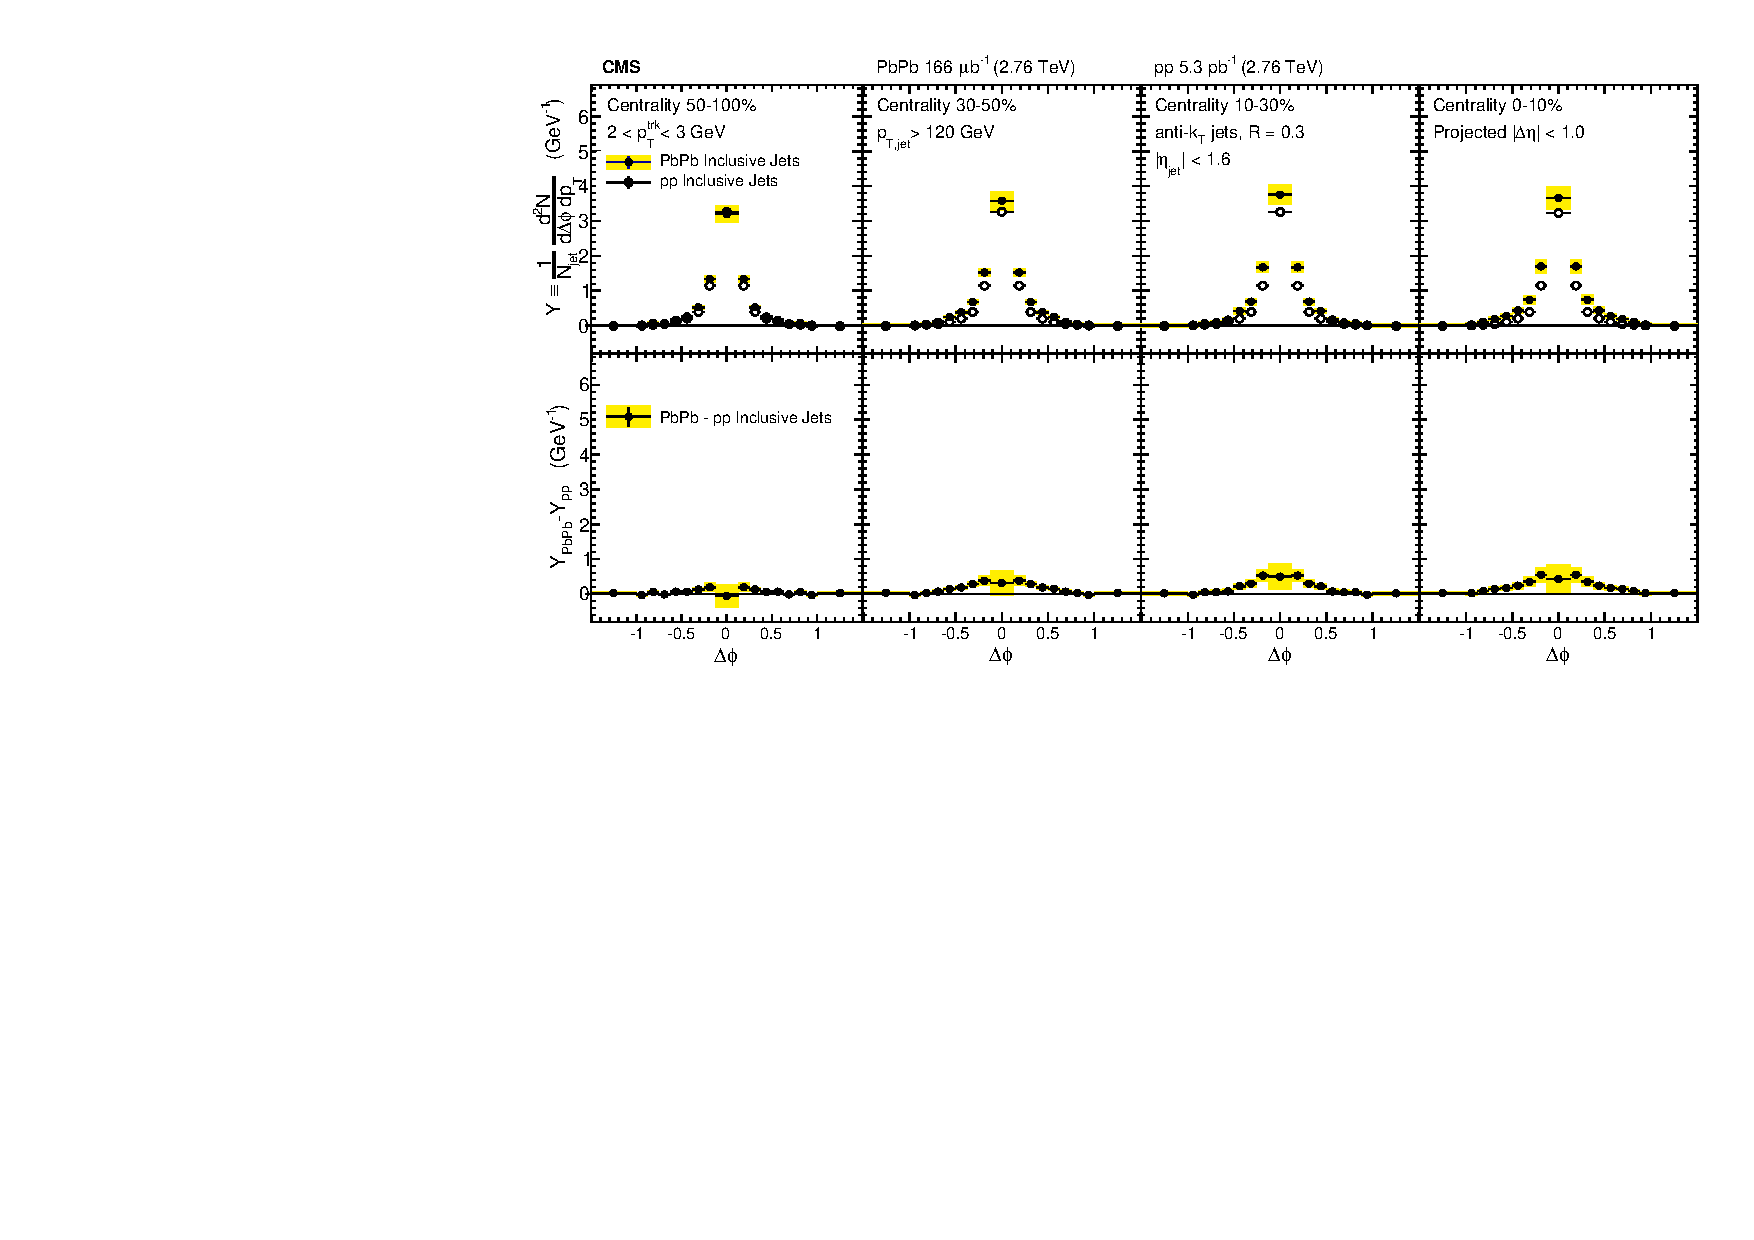
\includegraphics[width=0.99\textwidth]{figures/Results/PAS_Figure_4_TrkPt2_TrkPt3.pdf}
\caption[Inclusive jet $\Delta\phi$ correlations for tracks with $2 < p_{\rm T}^{\rm trk} < 3$ GeV at 2.76 TeV]{Symmetrized $\protect\Delta\phi$ distributions  (projected over $|\Delta\eta| < 1$) of background-subtracted particle yields correlated to PbPb and pp inclusive jets with $p_{\rm T} >$ 120 GeV are shown in the top panels for tracks with 2 $ < p_{\rm T}^{\rm trk} < $ 3 GeV.  The difference in PbPb and pp per-jet yields is shown in the bottom panels. The total systematic uncertainties are shown as shaded boxes, and statistical uncertainties are shown as vertical bars (often smaller than the symbol size).}
\label{fig:Inclusive_dPhi2} 
\end{center} 
\end{figure} 


\begin{figure}[hbt] 
\begin{center} 
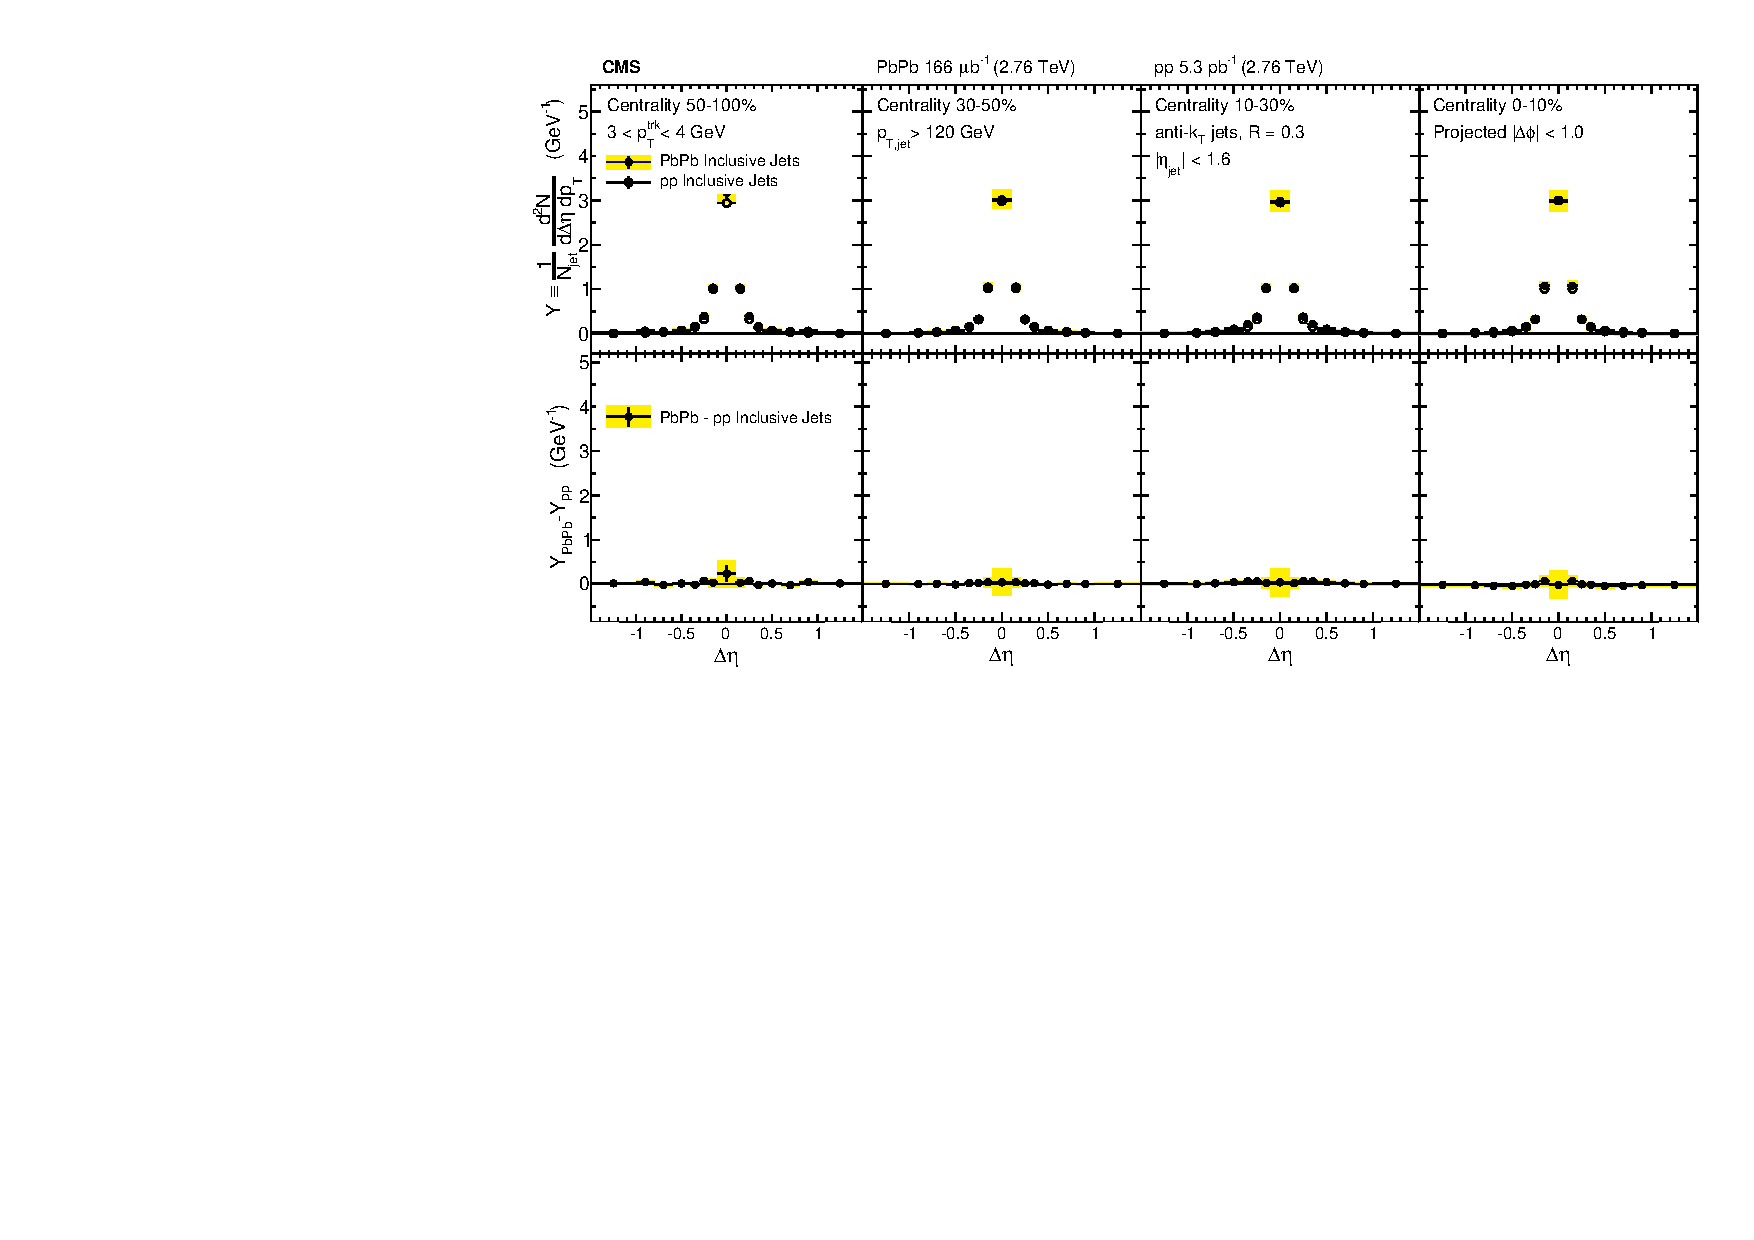
\includegraphics[width=0.99\textwidth]{figures/Results/PAS_Figure_3_TrkPt3_TrkPt4.pdf}
\caption[Inclusive jet $\Delta\eta$ correlations for tracks with $3 < p_{\rm T}^{\rm trk} < 4$ GeV at 2.76 TeV]{Symmetrized $\protect\Delta\eta$ distributions (projected over $|\Delta\phi| < 1$) of background-subtracted particle yields correlated to PbPb and pp inclusive jets with $p_{\rm T}>$ 120 GeV are shown in the top panels for tracks with 3 $ < p_{\rm T}^{\rm trk} < $ 4 GeV.  The difference in PbPb and pp per-jet yields is shown in the bottom panels. The total systematic uncertainties are shown as shaded boxes, and statistical uncertainties are shown as vertical bars (often smaller than the symbol size).}
\label{fig:Inclusive_dEta3}
\end{center} 
\end{figure} 

\begin{figure}[hbt] 
\begin{center} 
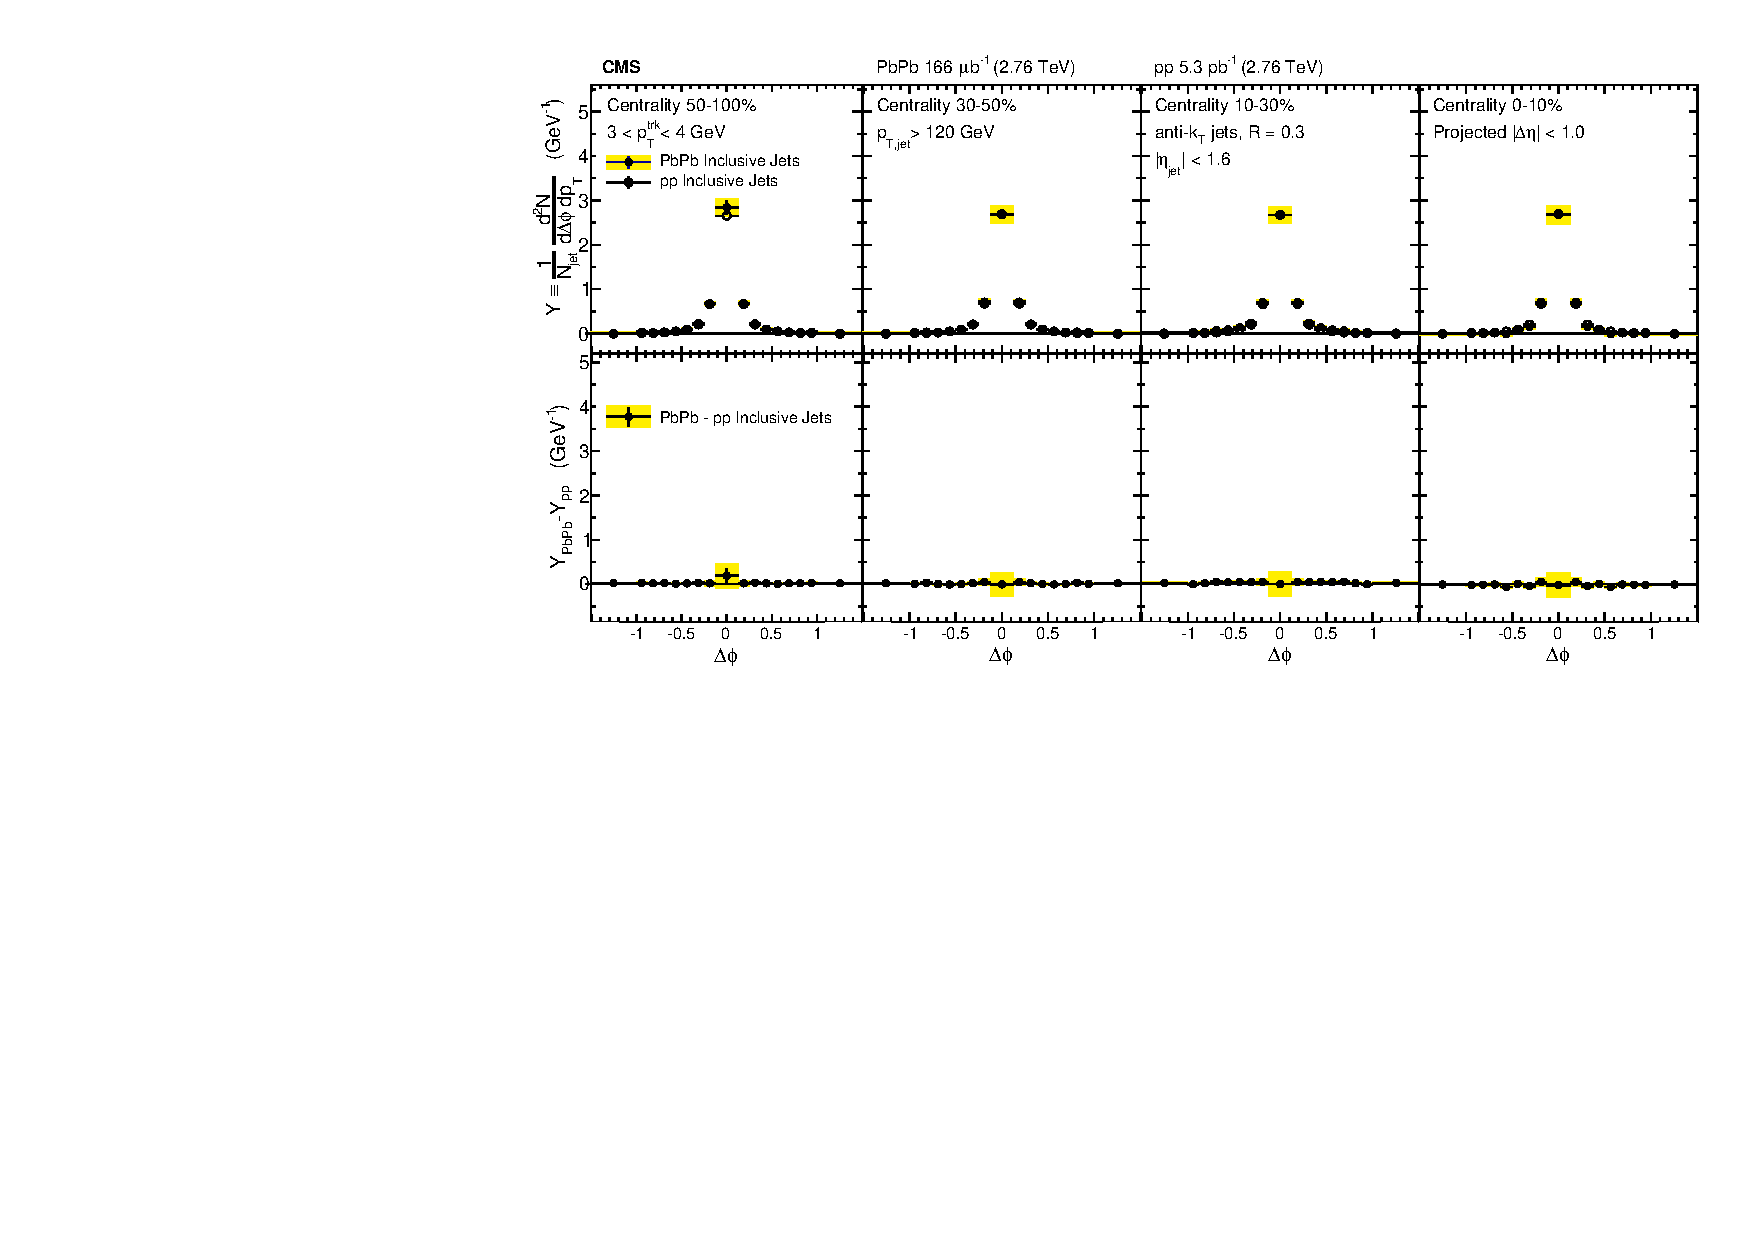
\includegraphics[width=0.99\textwidth]{figures/Results/PAS_Figure_4_TrkPt3_TrkPt4.pdf}
\caption[Inclusive jet $\Delta\phi$ correlations for tracks with $3 < p_{\rm T}^{\rm trk} < 4$ GeV at 2.76 TeV]{Symmetrized $\protect\Delta\phi$ distributions  (projected over $|\Delta\eta| < 1$) of background-subtracted particle yields correlated to PbPb and pp inclusive jets with $p_{\rm T} >$ 120 GeV are shown in the top panels for tracks with 3 $ < p_{\rm T}^{\rm trk} < $ 4 GeV.  The difference in PbPb and pp per-jet yields is shown in the bottom panels. The total systematic uncertainties are shown as shaded boxes, and statistical uncertainties are shown as vertical bars (often smaller than the symbol size).}
\label{fig:Inclusive_dPhi3} 
\end{center} 
\end{figure} 



\begin{figure}[hbt] 
\begin{center} 
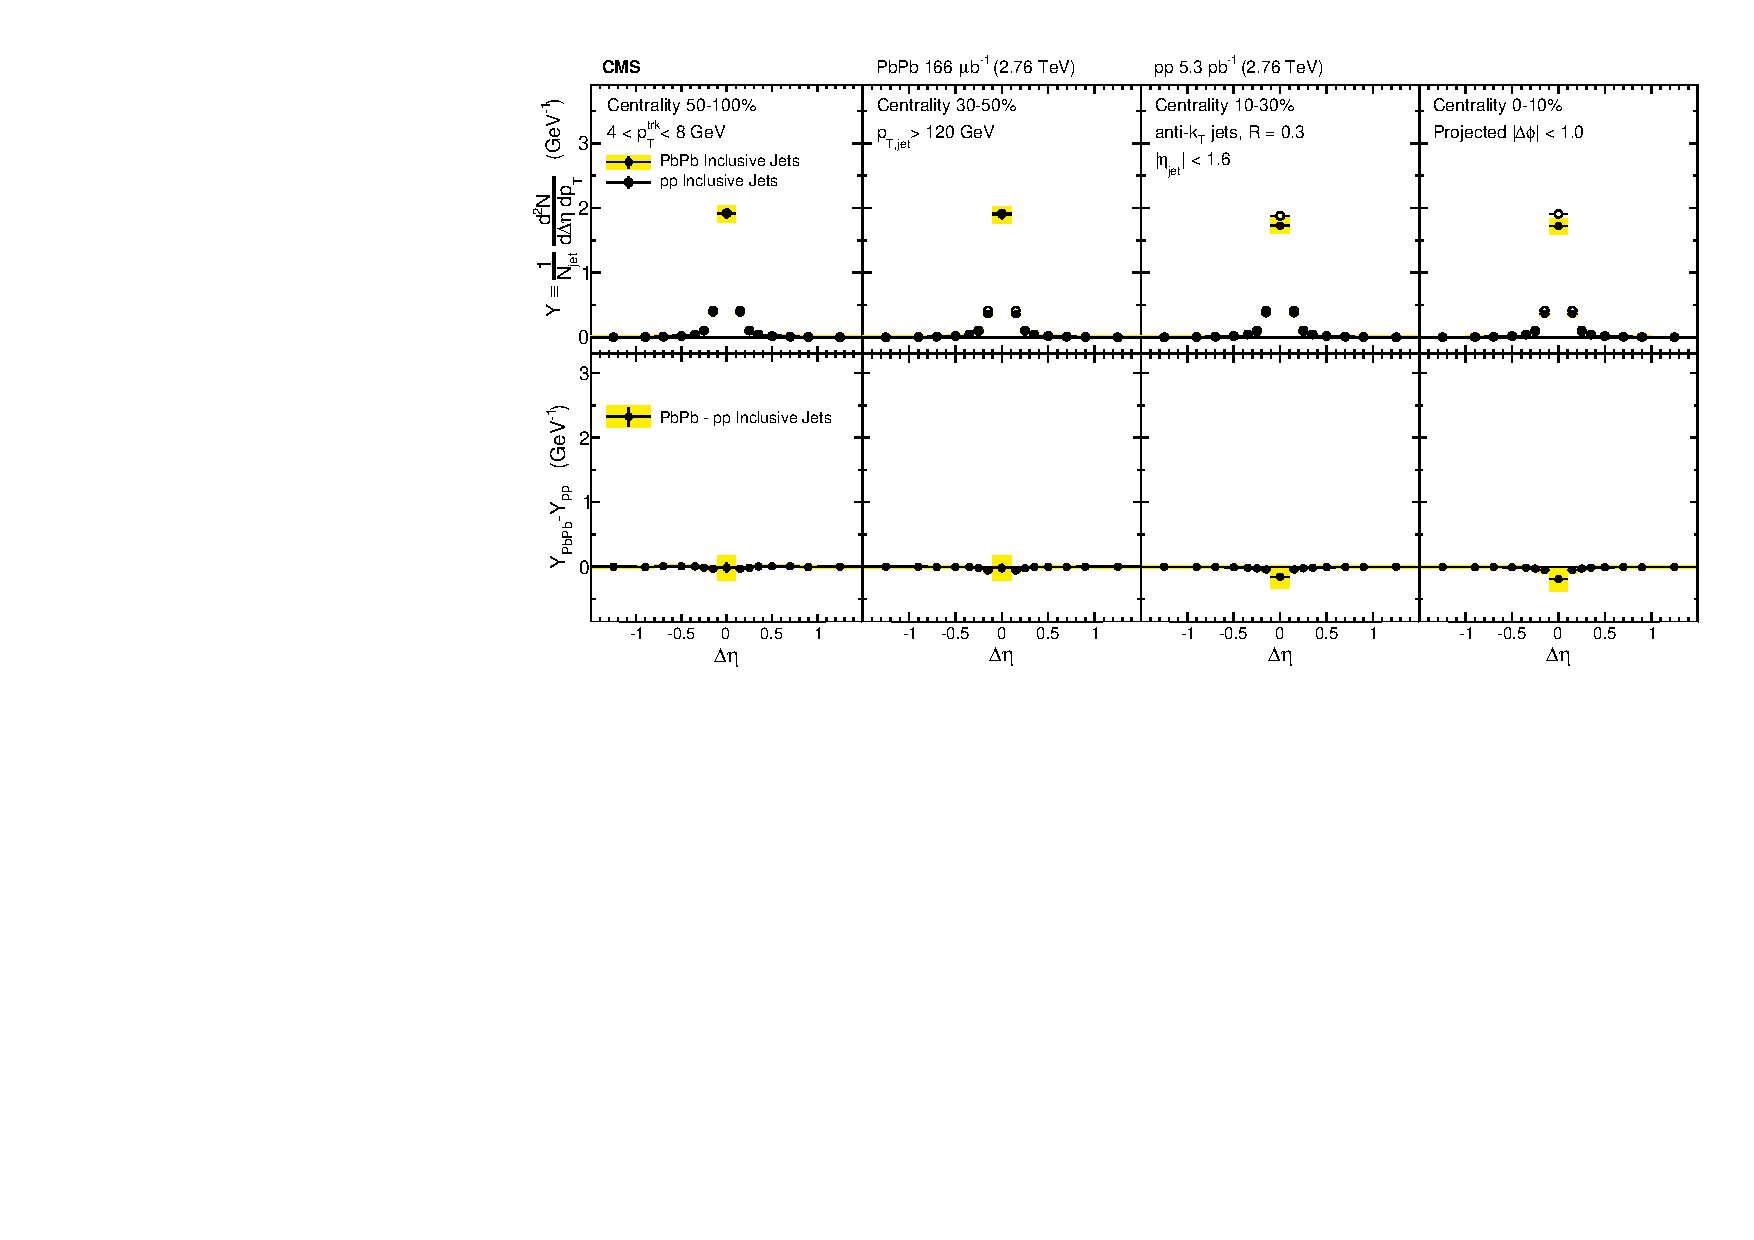
\includegraphics[width=0.99\textwidth]{figures/Results/PAS_Figure_3_TrkPt4_TrkPt8.pdf}
\caption[Inclusive jet $\Delta\eta$ correlations for tracks with $4 < p_{\rm T}^{\rm trk} < 8$ GeV at 2.76 TeV]{Symmetrized $\protect\Delta\eta$ distributions (projected over $|\Delta\phi| < 1$) of background-subtracted particle yields correlated to PbPb and pp inclusive jets with $p_{\rm T}>$ 120 GeV are shown in the top panels for tracks with 4 $ < p_{\rm T}^{\rm trk} < $ 8 GeV.  The difference in PbPb and pp per-jet yields is shown in the bottom panels. The total systematic uncertainties are shown as shaded boxes, and statistical uncertainties are shown as vertical bars (often smaller than the symbol size).}
\label{fig:Inclusive_dEta4}
\end{center} 
\end{figure} 

\begin{figure}[hbt] 
\begin{center} 
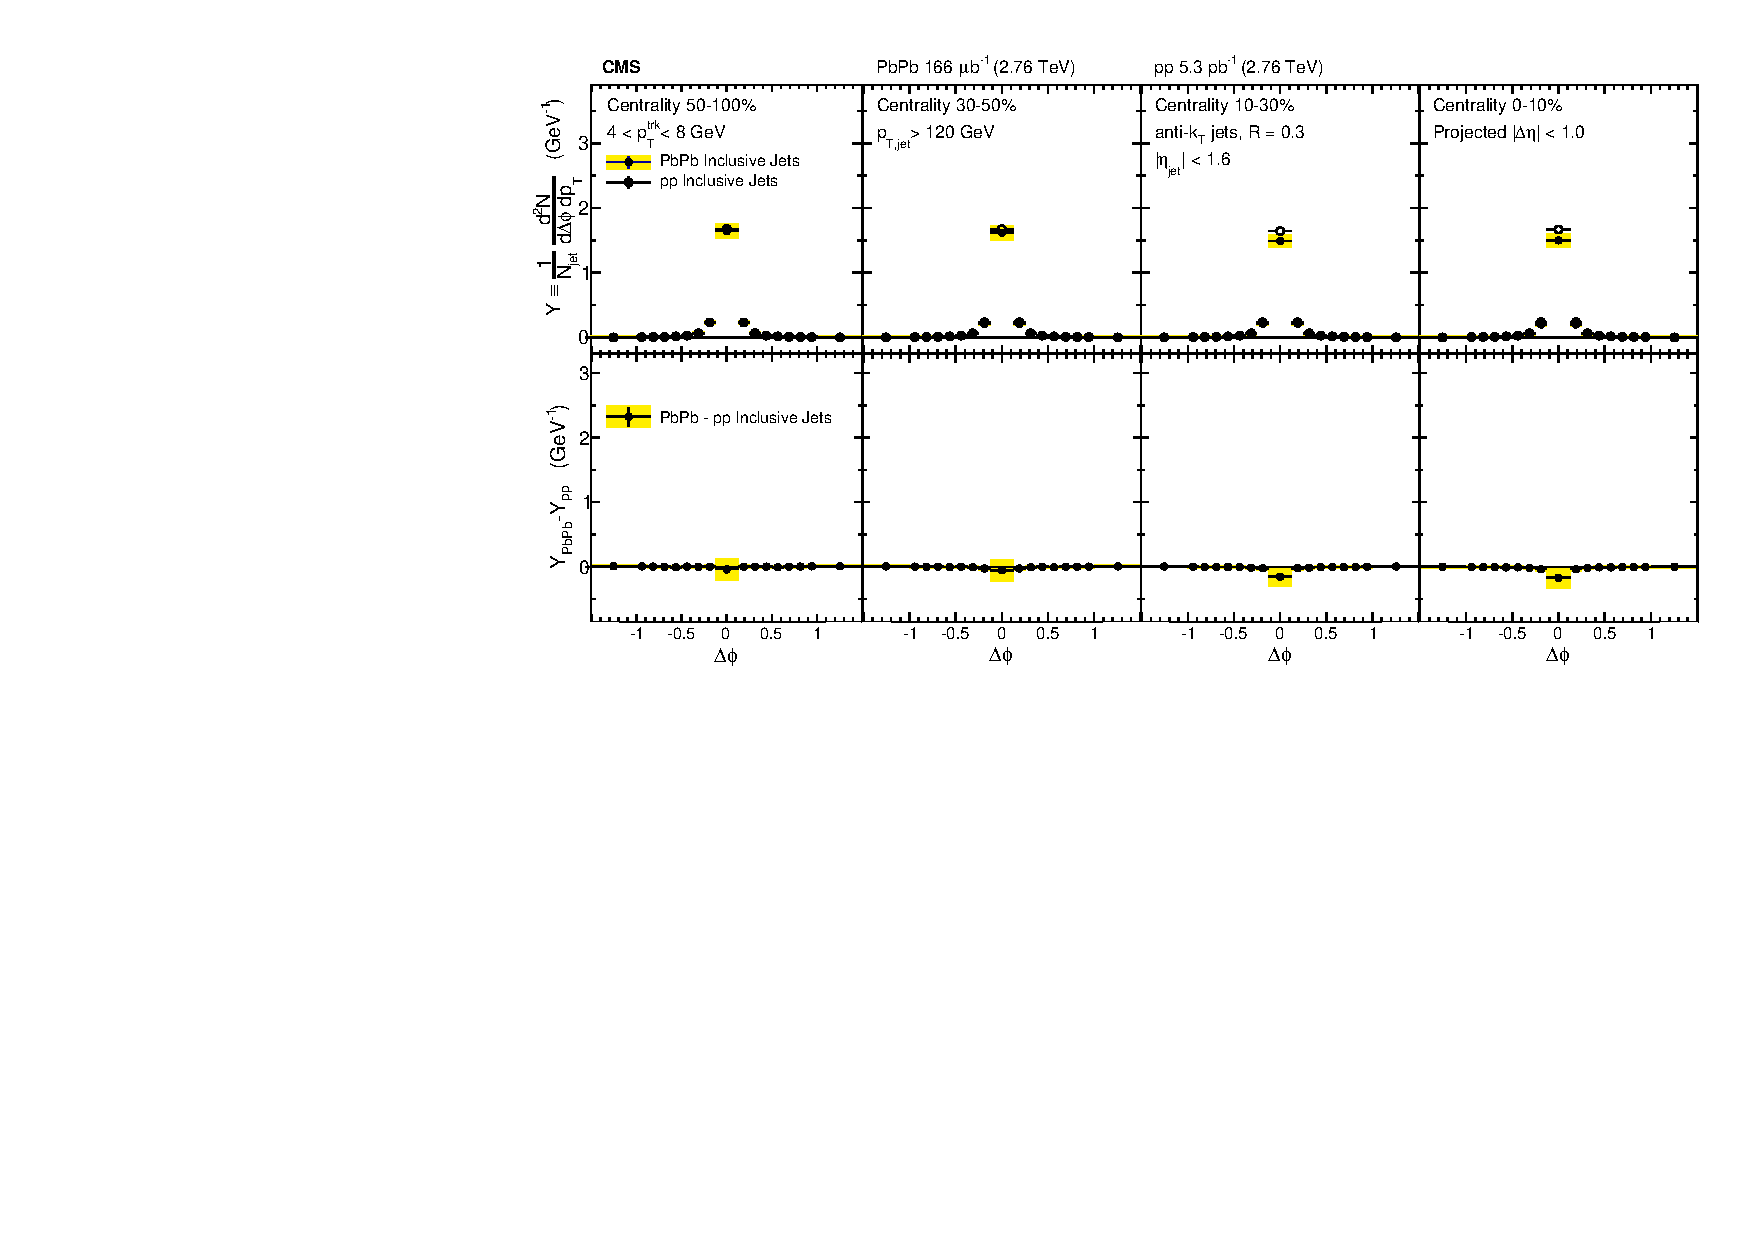
\includegraphics[width=0.99\textwidth]{figures/Results/PAS_Figure_4_TrkPt4_TrkPt8.pdf}
\caption[Inclusive jet $\Delta\phi$ correlations for tracks with $4 < p_{\rm T}^{\rm trk} < 8$ GeV at 2.76 TeV]{Symmetrized $\protect\Delta\phi$ distributions  (projected over $|\Delta\eta| < 1$) of background-subtracted particle yields correlated to PbPb and pp inclusive jets with $p_{\rm T} >$ 120 GeV are shown in the top panels for tracks with 4 $ < p_{\rm T}^{\rm trk} < $ 8 GeV.  The difference in PbPb and pp per-jet yields is shown in the bottom panels. The total systematic uncertainties are shown as shaded boxes, and statistical uncertainties are shown as vertical bars (often smaller than the symbol size).}
\label{fig:Inclusive_dPhi4} 
\end{center} 
\end{figure} 

 \begin{figure}[hbt]
    \begin{center}
       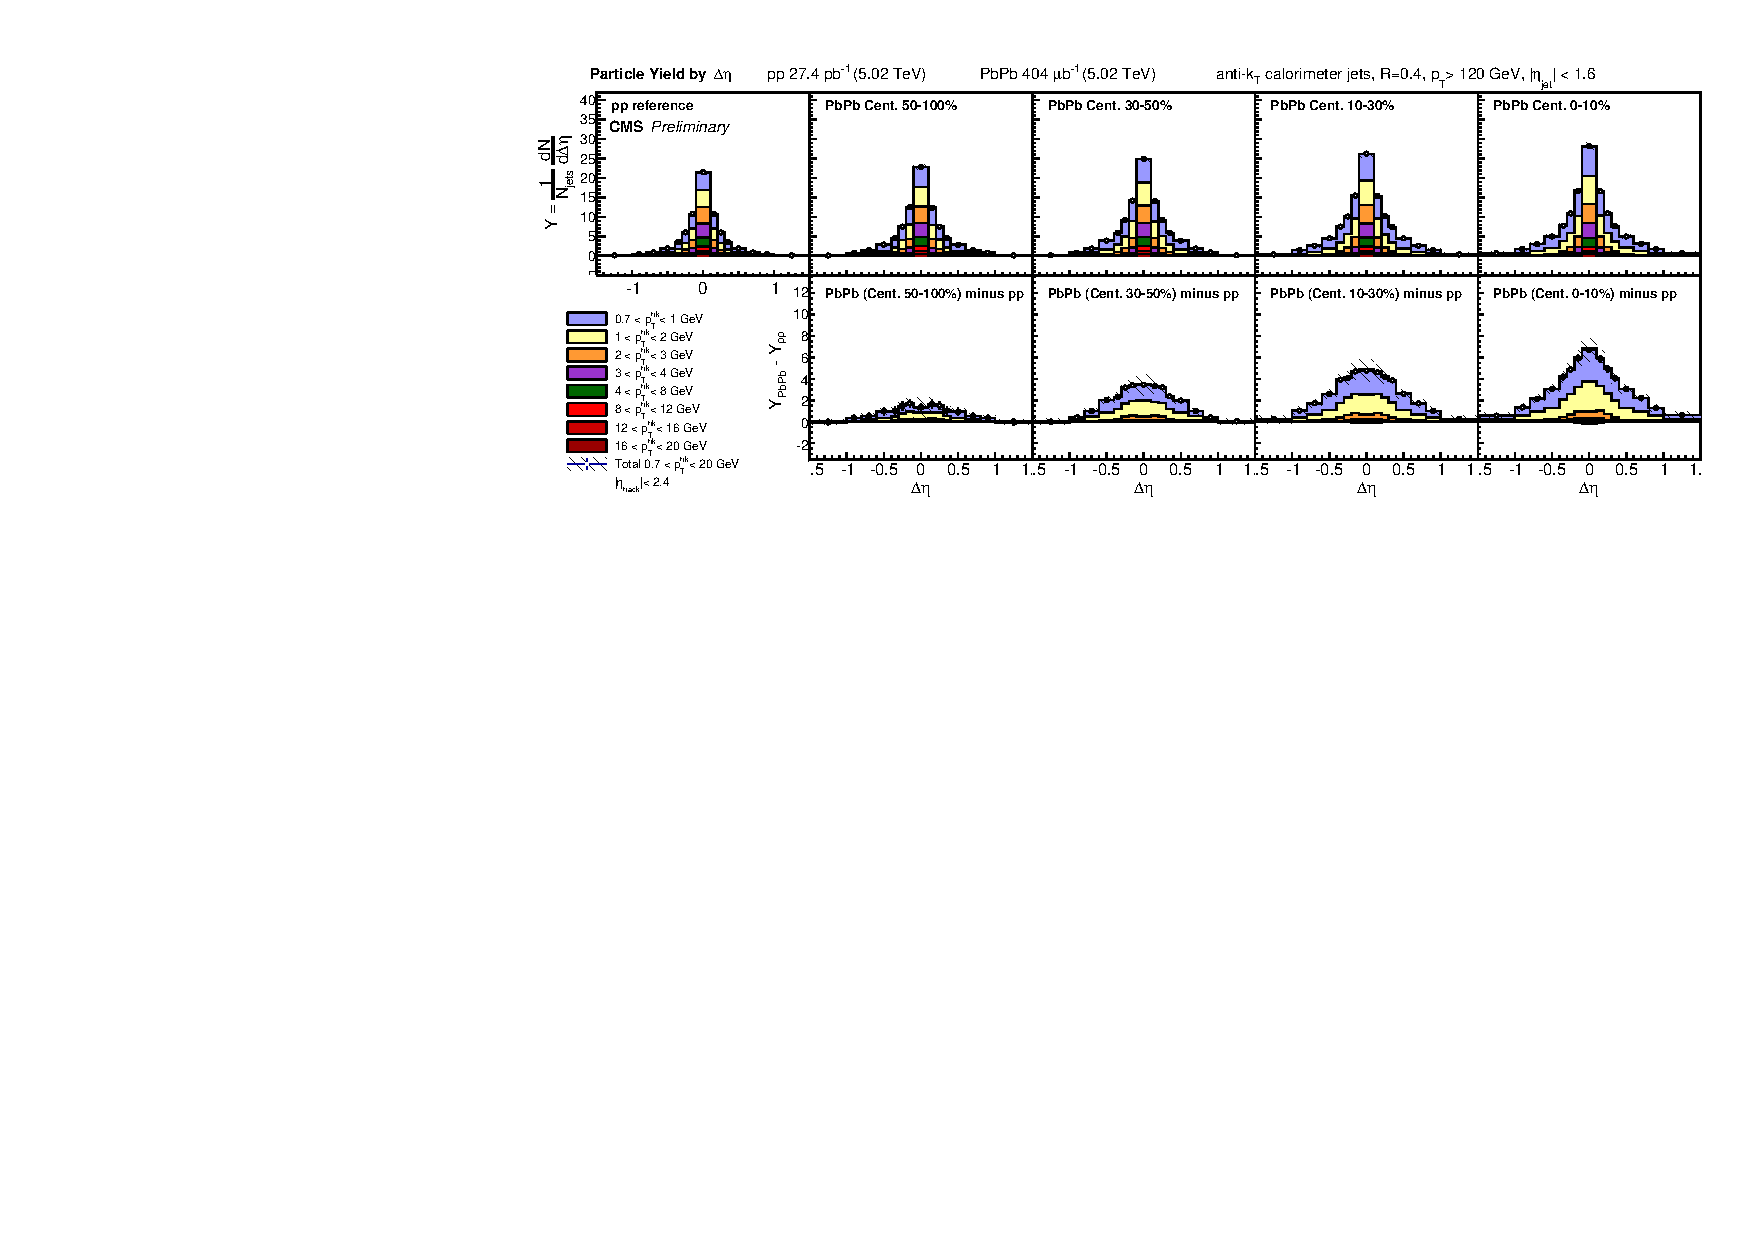
\includegraphics[width=0.99\textwidth]{figures/results/Yield_dEta_Stacked.pdf}
         \caption[Inclusive jet $\Delta\eta$ correlations at 5.02 TeV]{Top row: distributions of charged particle yields correlated to jets with $p_{\rm T} > 120$ GeV as a function of $\protect\Delta\eta$ (projected over $|\Delta\phi| < 1$), shown differentially for all $p_{\rm T}^{\rm trk}$ bins for pp, peripheral PbPb, and central PbPb data. Bottom row:  PbPb minus pp difference in these distributions.  Hatched lines on $p_{\rm T}^{\rm trk}$-inclusive points show total systematic uncertainties. }
       \label{fig:yield_deta_stacked}
    \end{center}
 \end{figure}
 
  \begin{figure}[hbt]
    \begin{center}
       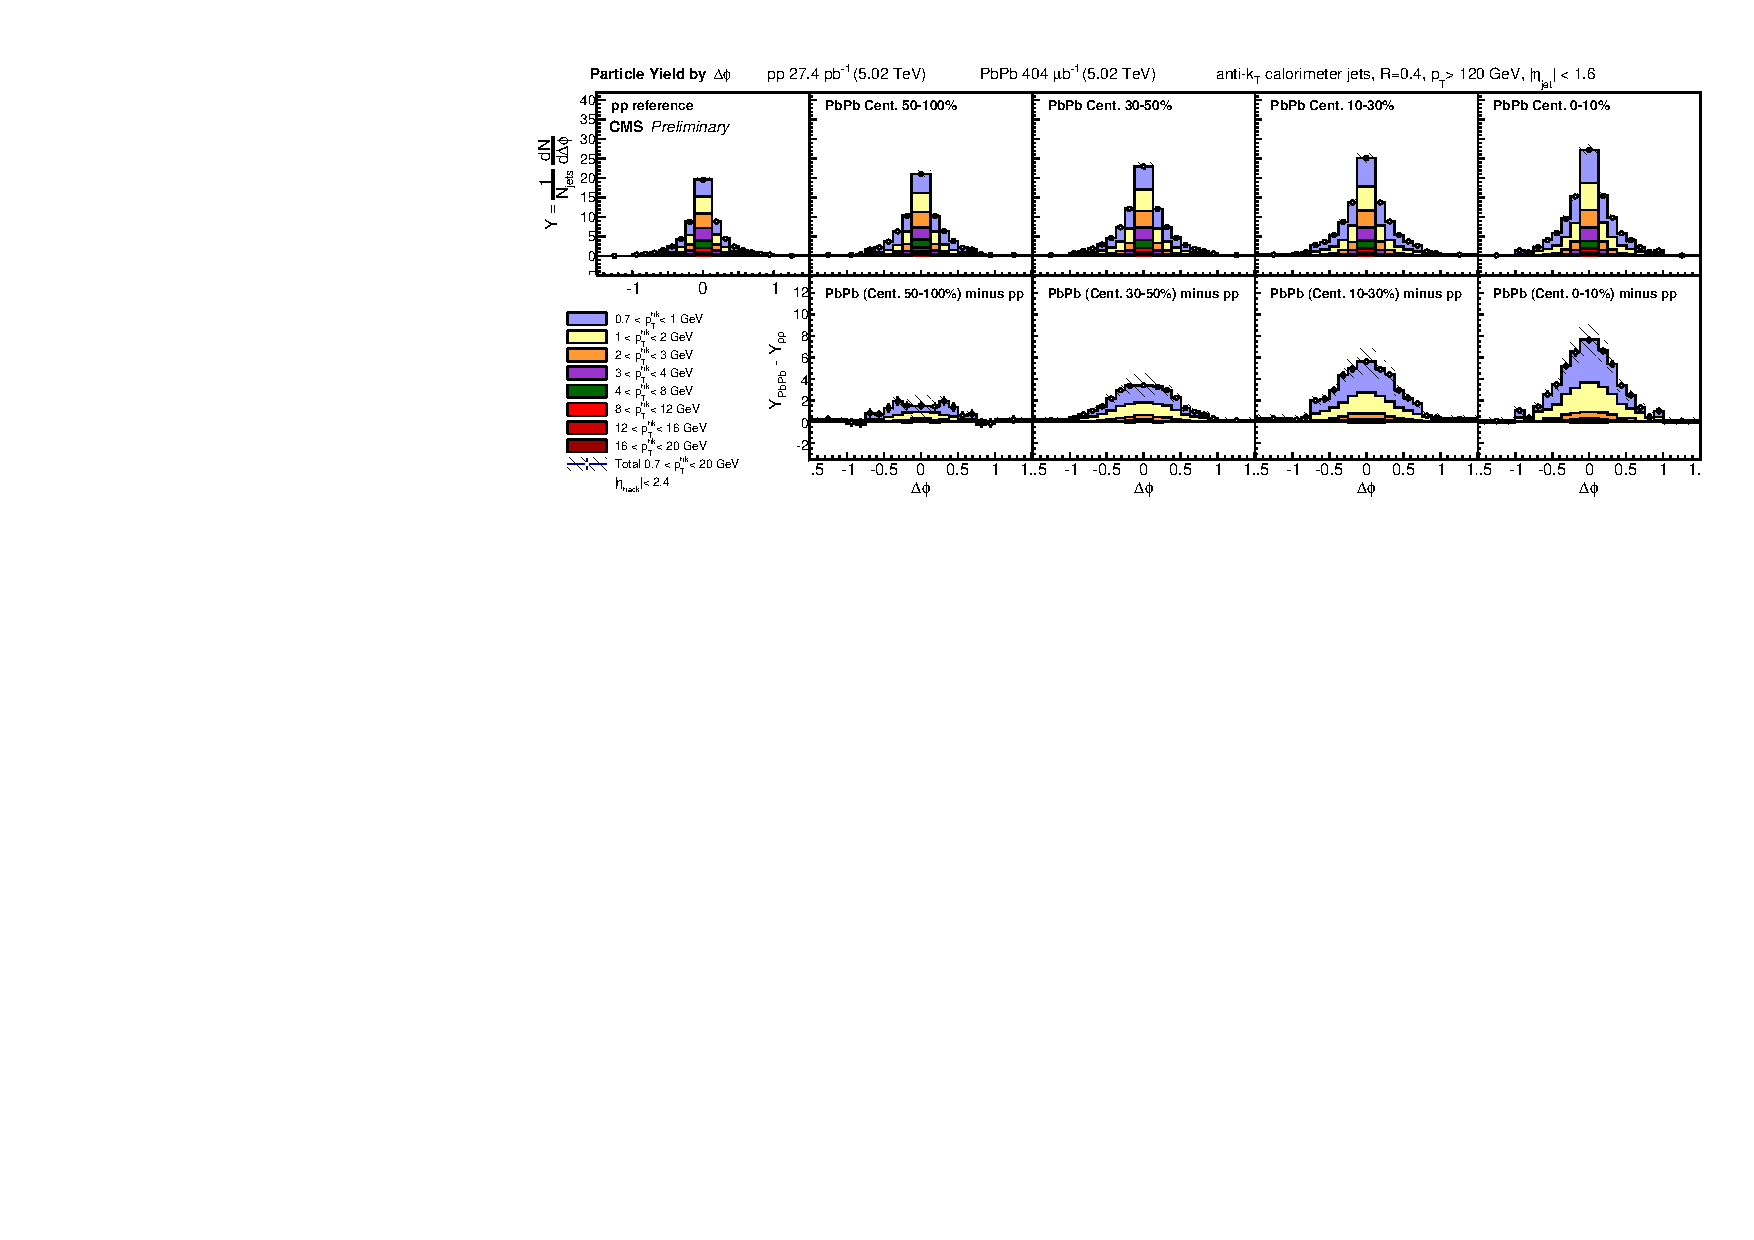
\includegraphics[width=0.99\textwidth]{figures/results/Yield_dPhi_Stacked.pdf}
         \caption[Inclusive jet $\Delta\phi$ correlations at 5.02 TeV]{Top row:  distributions of charged particle yields correlated to jets with $p_{\rm T} > 120$ GeV as a function of $\protect\Delta\phi$ (projected over $|\Delta\eta| < 1$), shown differentially for all $p_{\rm T}^{\rm trk}$ bins for pp, peripheral PbPb, and central PbPb data. Bottom row:  PbPb minus pp difference in these distributions.  Hatched lines on $p_{\rm T}^{\rm trk}$-inclusive points show total systematic uncertainties.}
       \label{fig:yield_dphi_stacked}
    \end{center}
 \end{figure}
 
  \begin{figure}[hbt]
    \begin{center}
       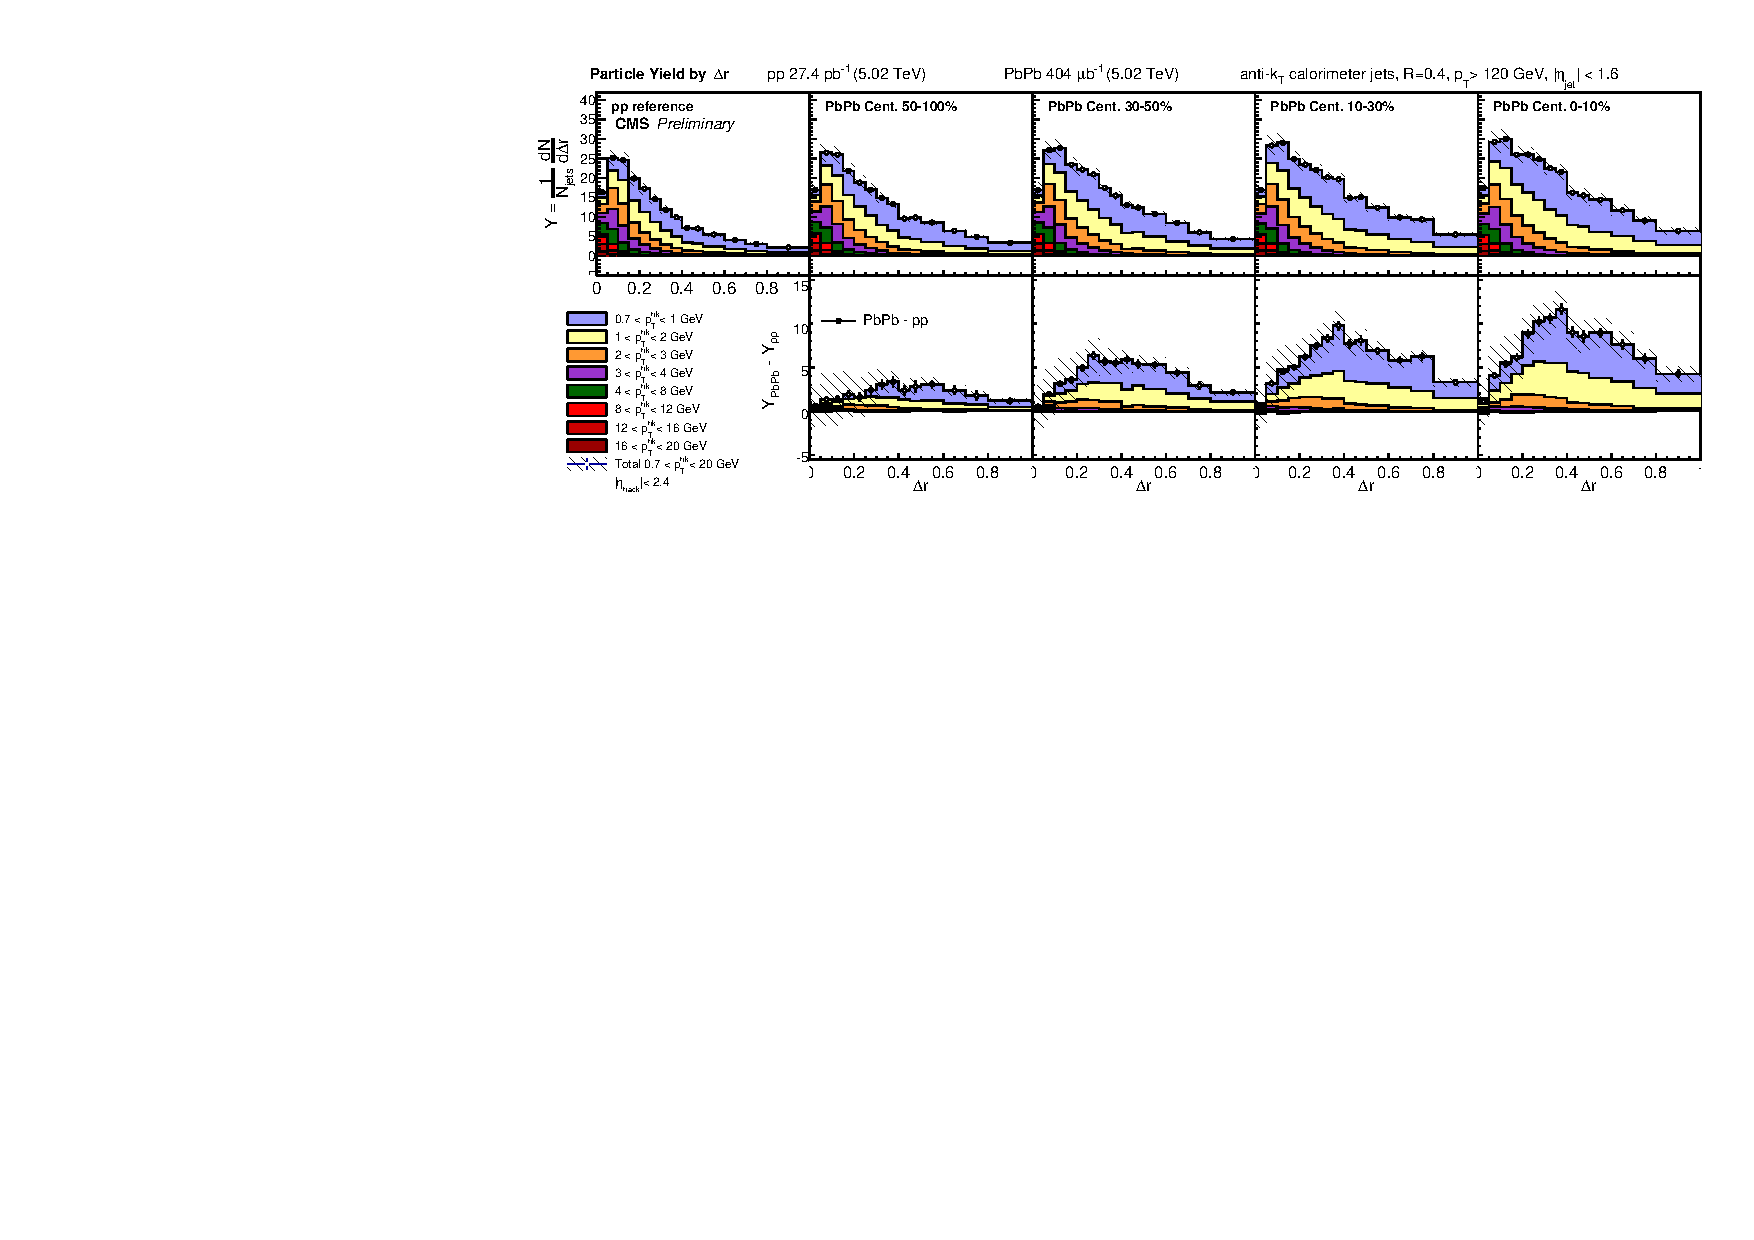
\includegraphics[width=0.99\textwidth]{figures/results/ParticleYield_by_dR.pdf}
         \caption[Inclusive jet distribution of charged particles as a function of $\Delta r$ at 5.02 TeV]{Top row:  distributions of charged particle yields correlated to jets with $p_{\rm T} > 120$ GeV as a function of $\protect\Delta r$, shown differentially for all $p_{\rm T}^{\rm trk}$ bins. Bottom row:  PbPb minus pp difference in these distributions. Hatched lines on $p_{\rm T}^{\rm trk}$-inclusive points show total systematic uncertainties.}
       \label{fig:yield_dr_stacked}
    \end{center}
 \end{figure}
 
 \clearpage
 
To summarize the magnitude of the modifications to particle yields in PbPb relative to pp colllisions, integrated yields as a function of $p_{\rm T}^{\rm trk}$ are presented in in the top panel of Fig.~\ref{fig:yield_integral}.  The bottom panel of Fig.~\ref{fig:yield_integral} shows differences PbPb--pp in total integrated particle yields in each $p_{\rm T}^{\rm trk}$ class for results at 5.02 TeV compared to 2.76 TeV results.  This quantifies the low-$p_{\rm T}$ excess in central PbPb collisions to as many as 4 additional particles (in central PbPb relative to pp reference) per unit of $p_{\rm T}^{\rm trk}$ in the lowest $p_{\rm T}^{\rm trk}$ bin.  This excess decreases smoothly with $p_{\rm T}^{\rm trk}$ in each centrality bin, until the 4--8 GeV central PbPb bin is consistent with or slightly depleted relative to pp reference.  For tracks with  $p_{\rm T}^{\rm trk} > 8 $ GeV, there is no evident modification in PbPb compared to pp.  Excess yields do not exhibit significant dependence on collision energies; particle yields at low-$p_{\rm T}^{\rm trk}$ are consistently larger at 5.02 TeV than at 2.76 TeV, but within the systematic uncertainties of the two measurements. 

 
  \begin{figure}[hbt]
    \begin{center}
       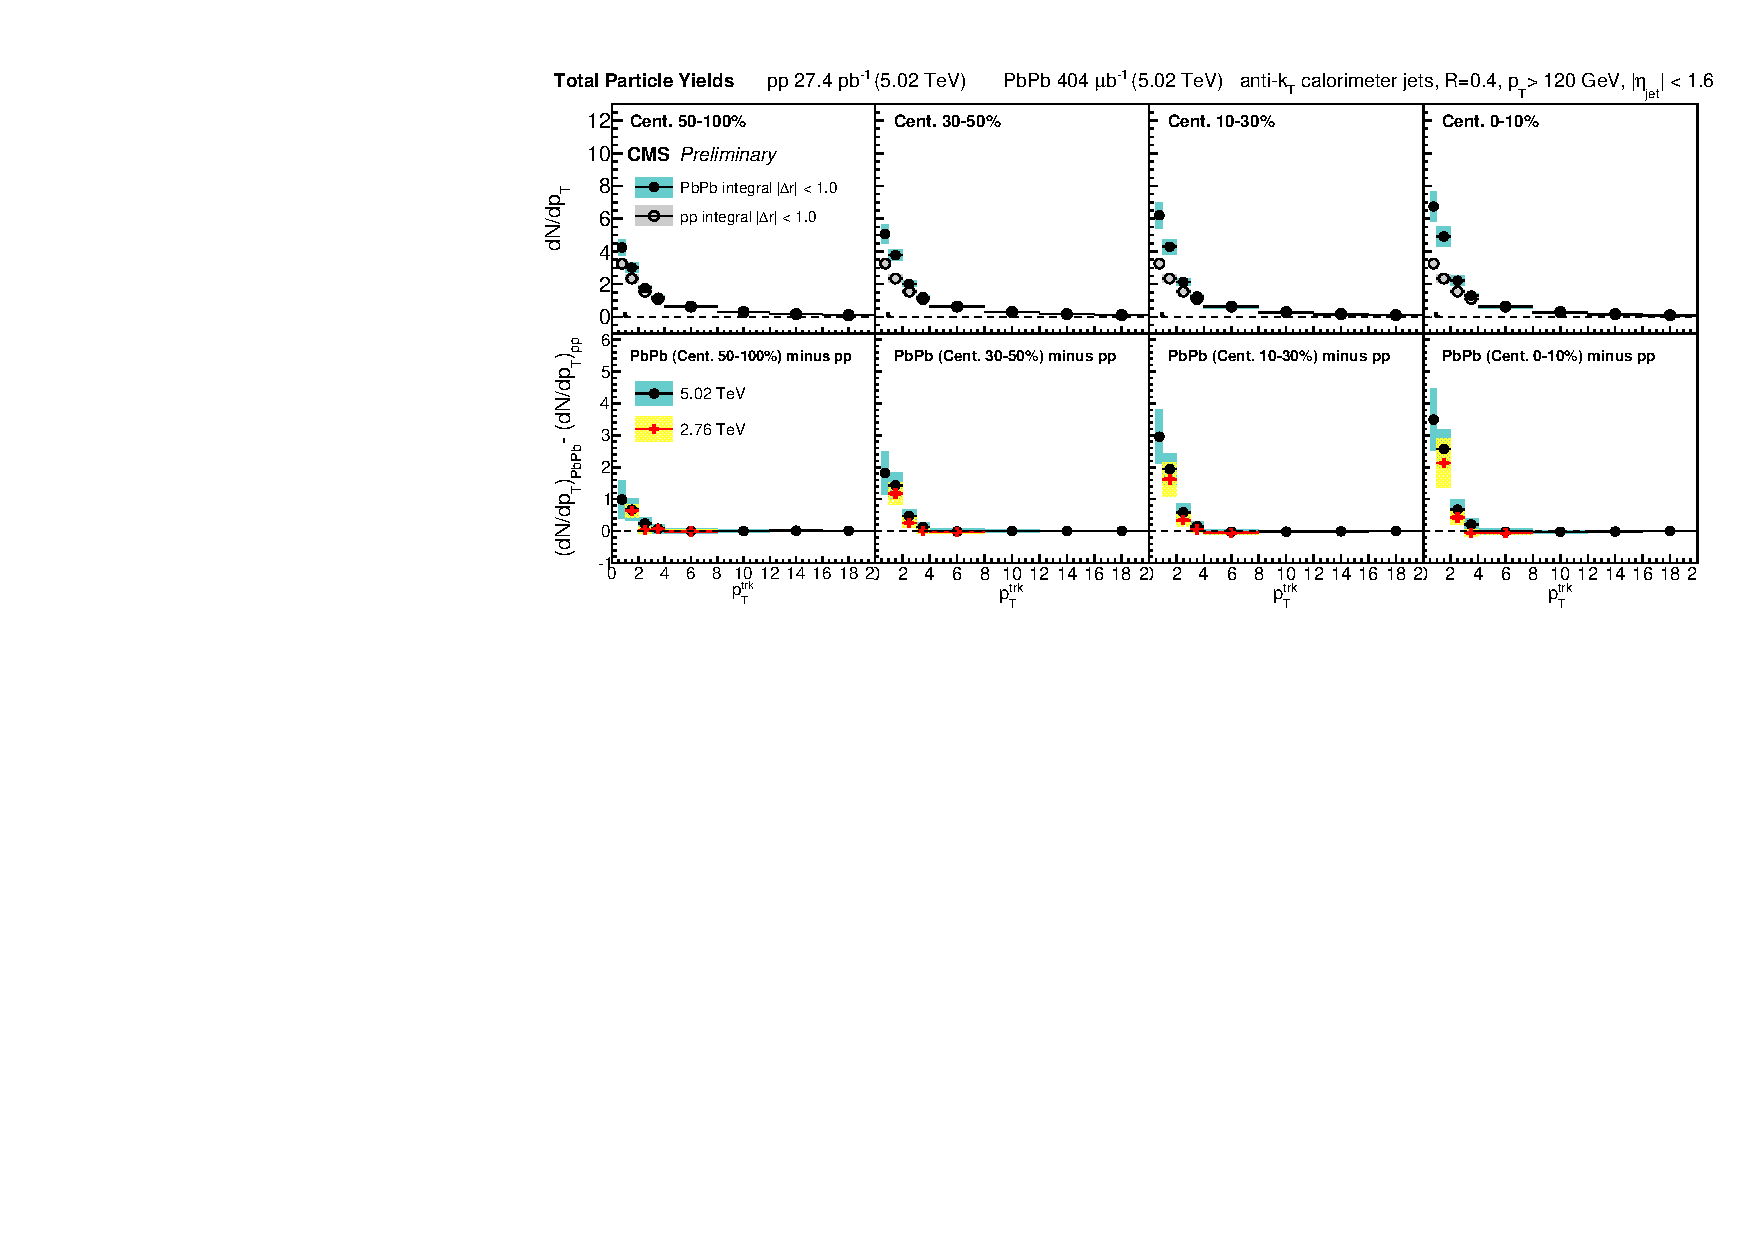
\includegraphics[width=0.99\textwidth]{figures/results/Integral_dR.pdf}
         \caption[Integrated inclusive jet charged particle yields at 2.76 and 5.02 TeV]{Top row: integrated yields of charged particle yields correlated to jets with $p_{\rm T} > 120$ GeV as a function of $p_{\rm T}^{\rm trk}$ bins for PbPb data, compared to pp reference.  Bottom row:  integrated excess yield, PbPb minus pp. New measurements of excess yields at 5.02 TeV are compared to those measured at 2.76 TeV.}       \label{fig:yield_integral}
    \end{center}
 \end{figure}


\clearpage

\subsection{Dijet correlation results at 2.76 TeV}
\label{sec:dijet_corr}

In the studies of charged-particle yields correlated to an inclusive sample of jets with $p_{\rm T} > 120$ GeV presented above, jet quenching is evident in the redistribution of $p_{\rm T}^{\rm trk}$ from harder to softer particles, and particularly in the observed centrality-dependent excess of low-$p_{\rm T}^{\rm trk}$ particle yields.  Jet quenching effects may be further probed by considering charged-particle yields correlated to each jet axis in dijet events.  Requiring events with two back-to-back jets (leading jet $p_{\rm T,1} > 120$ GeV, subleading jet $p_{\rm T,2} > 50$ GeV, $\Delta\phi_{\rm 1,2} > \frac{5\pi}{6}$), we construct separate correlations to the leading and the subleading jet axes.  In pp data, most dijets are balanced while in central PbPb a greater fraction of dijet pairs are unbalanced (as discussed in Sec.~\ref{sec:jet_sel}), suggesting that central PbPb data contains a significant fraction of dijet pairs in which the highest- and second-highest-$p_{\rm T}$ hard-scattering products had similar transverse momenta, but in which one jet experienced a greater path-length through the medium and correspondingly greater quenching.  This is expected to correspond to a ``surface-bias'' toward leading jets with very short path-lengths through the medium, that might be expected to cause minimal quenching in the leading jet sample.  It is therefore interesting to separately compare charged-particle distributions with respect to the leading and subleading jet axes in PbPb and pp data to look for evidence of path-length dependence in jet quenching.  

Figures~\ref{fig:fig2_dEta1} and~\ref{fig:fig2_dPhi1} show these correlation patterns in $\Delta\eta$ and $\Delta\phi$, respectively, for the $1 < p_{\rm T}^{\rm trk}$ GeV range in which the greatest quenching was evident in the 2.76 TeV inclusive jet studies.  As expected, quenching effects are greater for subleading than leading jets, as evident in larger excesses of soft particles in subleading jet correlations (while retaining the same centrality trends and gaussian-like distributions observed for the inclusive jet sample).  However, leading jets exhibit evidence of quenching as well, showing similar soft-particle excesses to those observed in the inclusive sample.  To quantitatively compare subleading and leading jet modifications to those in the inclusive jet sample, Fig.~\ref{fig:Excess_vs_trkpt} shows integrated particle yields for all three jet samples at 2.76 TeV.  Here it is clear that leading jets show similar PbPb--pp modifications to those observed in the inclusive sample, with approximately 2 excess particles in PbPb compared to pp data at lowest-$p_{\rm T}^{\rm trk}$, while the subleading jet sample shows as manty as 4 excess particles in PbPb compared to pp data at lowest-$p_{\rm T}^{\rm trk}$.

\begin{figure}[hbtp]
\begin{center}
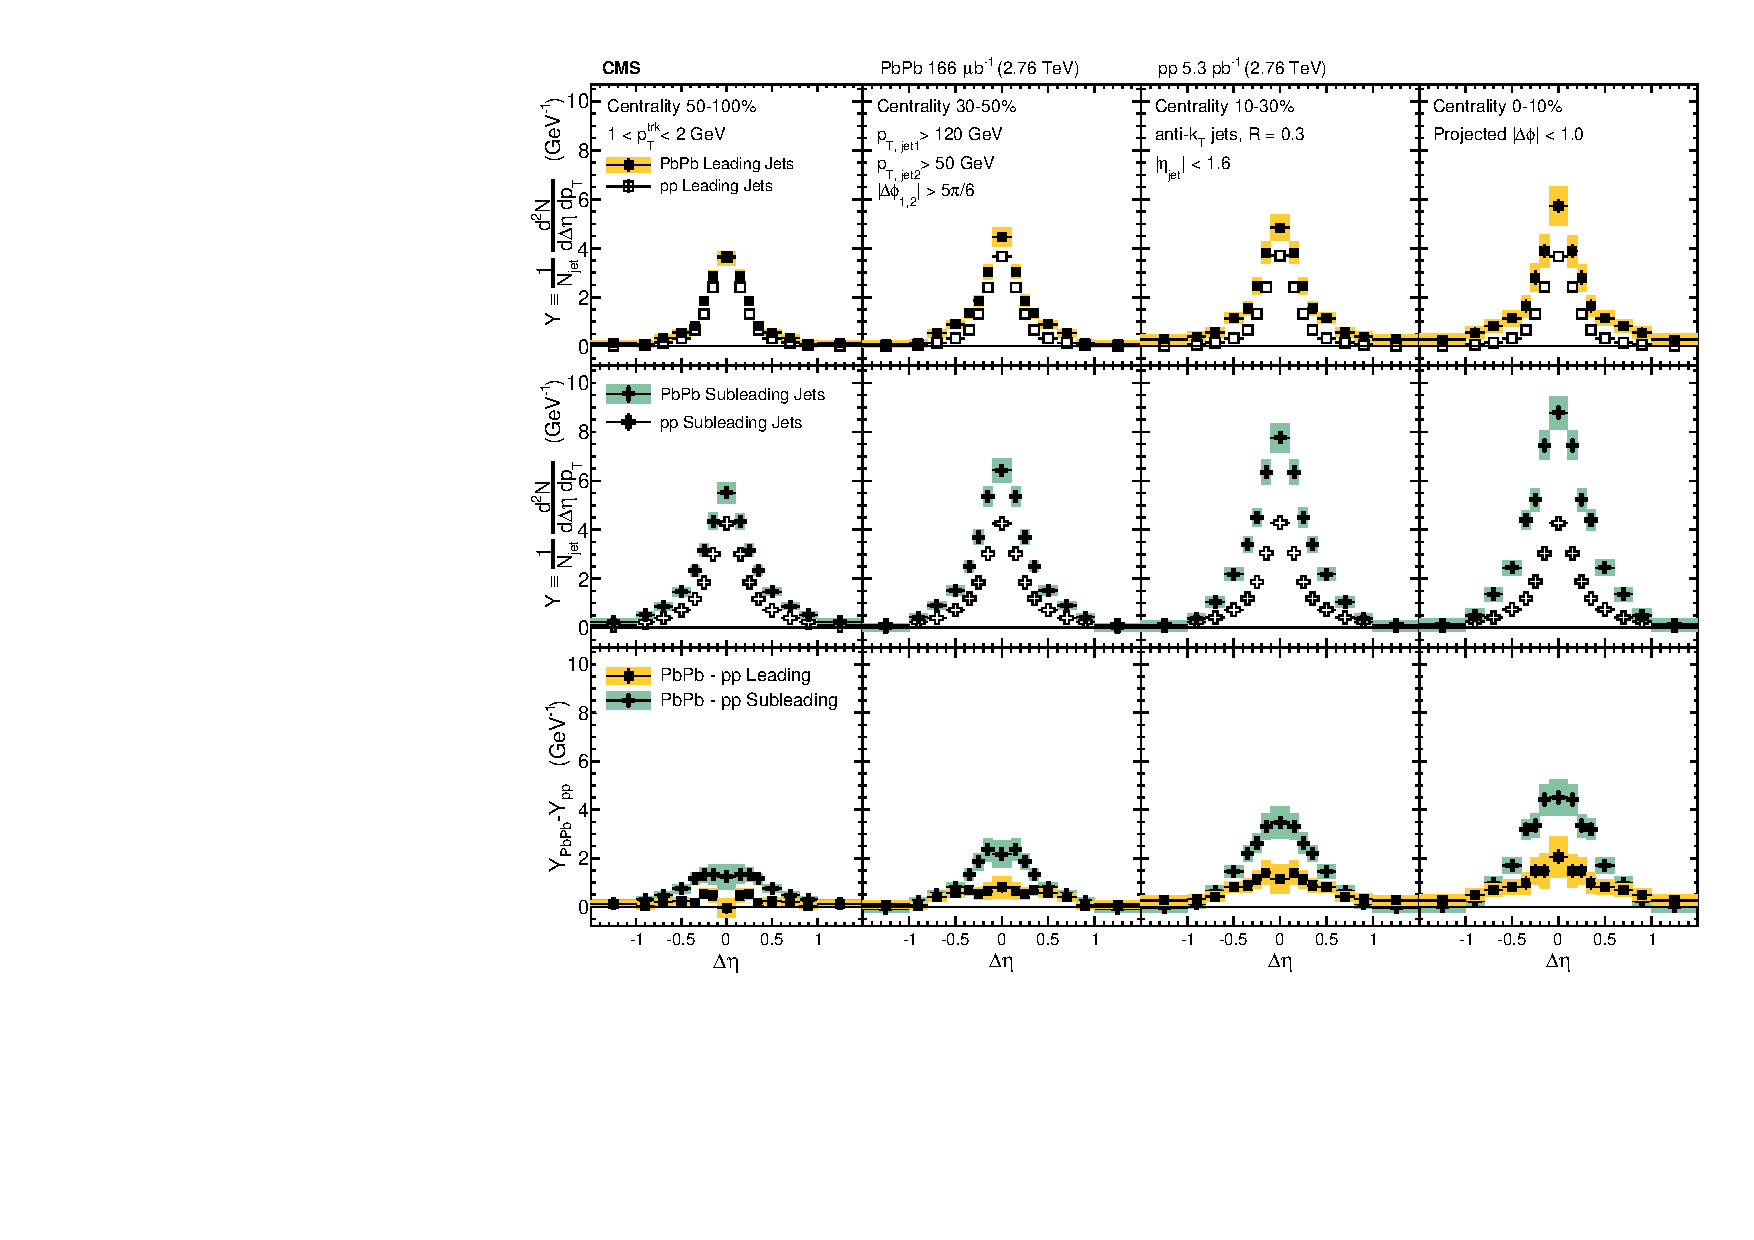
\includegraphics[width=0.99\textwidth]{figures/Results/PAS_Figure_5_TrkPt1_TrkPt2.pdf}
\caption[Dijet $\Delta\eta$ correlations for tracks with $1 < p_{\rm T}^{\rm trk} < 2$ GeV at 2.76 TeV]{The top panels show the $\protect\Delta\eta$ distributions (projected over $|\Delta\phi| < 1$) of charged-particle background-subtracted yields correlated to PbPb and pp leading jets with $p_{\rm T, jet1}>$ 120~GeV.  The middle panels show the same distributions for subleading jets with $p_{\rm T, jet2}>$ 50~GeV, and the bottom panels show the difference PbPb minus pp for both leading and subleading jets. The total systematic uncertainties are shown as shaded boxes, and statistical uncertainties are shown as vertical bars (often smaller than the symbol size).}
 \label{fig:fig2_dEta1}
   \end{center}
\end{figure}

\begin{figure}[hbtp]
\begin{center}
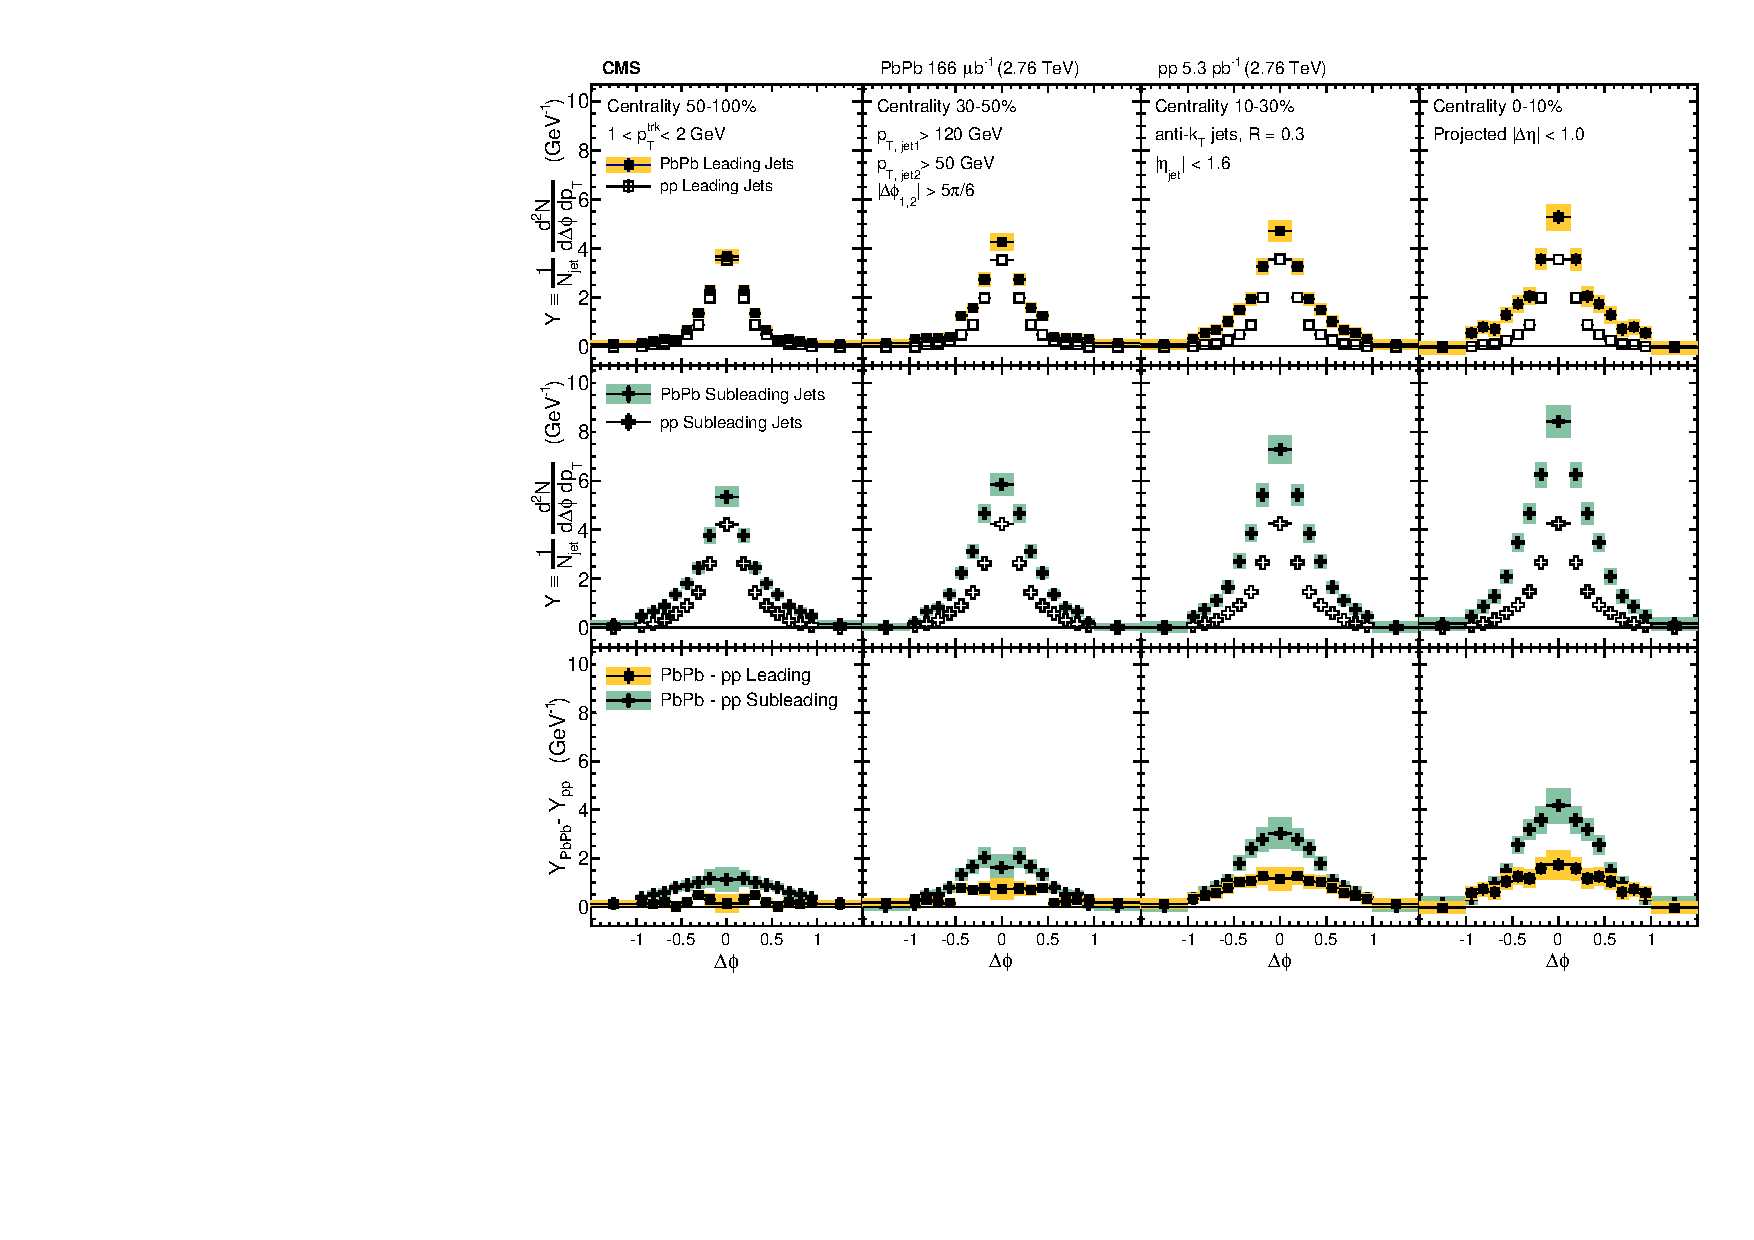
\includegraphics[width=0.99\textwidth]{figures/Results/PAS_Figure_6_TrkPt1_TrkPt2.pdf}
     \caption[Dijet $\Delta\phi$ correlations for tracks with $1 < p_{\rm T}^{\rm trk} < 2$ GeV at 2.76 TeV]{The top panels show the $\protect\Delta\phi$ distributions (projected over $|\Delta\eta < 1$) of charged-particle background-subtracted yields correlated to PbPb and pp leading jets with $p_{\rm T, jet1}>$ 120~GeV.  The middle panels show the same distributions for subleading jets with $p_{\rm T, jet2}>$ 50~GeV, and the bottom panels show the difference PbPb minus pp for both leading and subleading jets. The total systematic uncertainties are shown as shaded boxes, and statistical uncertainties are shown as vertical bars (often smaller than the symbol size).}
      \label{fig:fig2_dPhi1}
   \end{center}
\end{figure}

\begin{figure}[hbtp]
\begin{center}
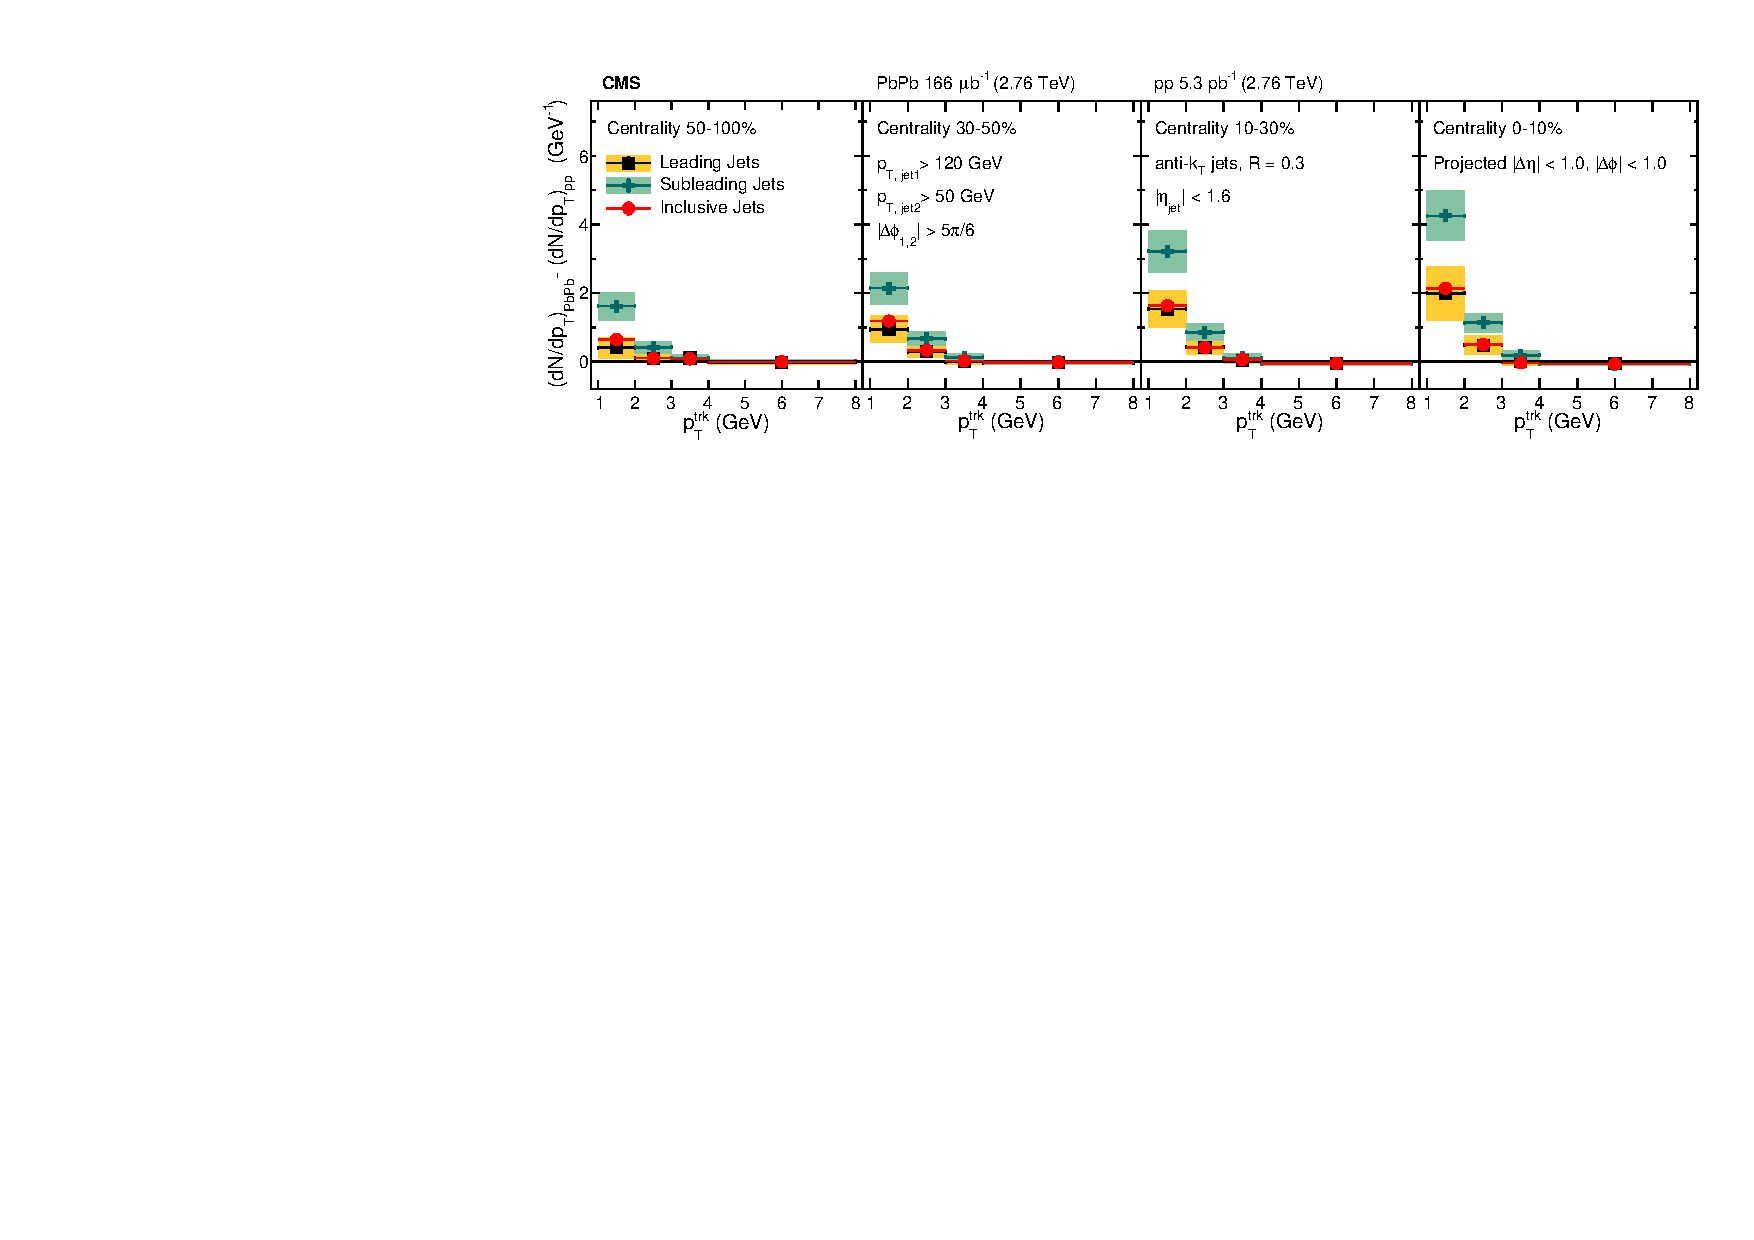
\includegraphics[width=0.99\textwidth]{figures/Results/PAS_Figure_7_WithInclusive.pdf}
\caption[Integrated charged particle yields for inclusive, leading, and subleading jets]{Total excess correlated yield observed in the PbPb data with respect to the reference measured in pp collisions, shown as a function of track $p_{\rm T}$ in four different centrality intervals (0--10\%, 10--30\%, 30--50\%, 50--100\%) for both leading jets with $p_{\rm T, jet1}> $120~GeV and subleading jets with $p_{\rm T, jet2}>$ 50~GeV. The total systematic uncertainties are shown as shaded boxes, and statistical uncertainties are shown as vertical bars (often smaller than the symbol size).}
\label{fig:Excess_vs_trkpt}
\end{center}
\end{figure}

\clearpage

In addition to characterizing the magnitude of jet quenching products (via the centrality-dependent excess of low-$p_{\rm T}^{trk}$ tracks greatest in correlations to subleading jets but also present in leading jet correlations), modifications to charged-particle correlated yields may also be characterized by their widths.  These studies are are relevant to look for the presence and extent of jet peak broadening due to medium interactions, and can be used to distinguish between different models for jet-medium interaction and medium-modified jet radiation.  In order to characterize correlation widths, correlations are fit to double-gaussian functions (all $\Delta\eta$ fits are shown in Appendix~\ref{app:width_determination} for illustration), and the width ($\sigma$) of these fits is obtained as the range in $|\Delta\eta|$ or $|\Delta\phi|$ containing 67\% of the total yield under the fit curve.   To obtain systematic uncertainties on these fits, points are varied up and down by their systematic uncertainties, and widths are re-calculated from these varied distributions.  

Figures~\ref{fig:Width_eta_lead} and~\ref{fig:Width_phi_lead} show correlation widths in $\Delta\eta$ and $\Delta\phi$ for leading jets in PbPb and pp data at 2.76 TeV.   At low-$p_{\rm T}^{\rm trk}$ there is a significant broadening evident in central PbPb data when compared to pp data, with this broadening decreasing in more peripheral collisions and with increasing $p_{\rm T}^{\rm trk}$ (with similar trends to those exhibited by correlated yield magnitudes).  Widths and width modifications are similar in $\Delta\eta$ and $\Delta\phi$, but slightly broader in $\Delta\phi$ for PbPb data.  These leading jet correlation widths and width modifications may also be compared to subleading jet correlation widths and width modifications, shown in Figs.~\ref{fig:Width_eta_sub} and~\ref{fig:Width_phi_sub}.  In peripheral PbPb data subleading and leading correlation widths are similar, but subleading jet PbPb correlation widths exhibiting less centrality dependence than leading jet correlation widths so that leading jet correlations in central PbPb data are slightly broader than than subleading jet correlations (but not significantly so, when taking into account the systematic uncertainties on both measurements).  Subleading jet peaks in pp data are, however, significantly broader than leading jet peaks in pp data--as is to be expected since the kinematic selection defining subleading jet as that with lower-$p_{\rm T}$, also implies that subleading jets will on average have softer fragmentation than leading jets.  Since subleading pp jets are broader than leading pp jets while subleading and leading jets have similar widths in PbPb, the jet peak broadening quantified as the PbPb--pp difference in widths is greater for leading jets than for subleading jets.  

\begin{figure}[hbtp]
\begin{center}
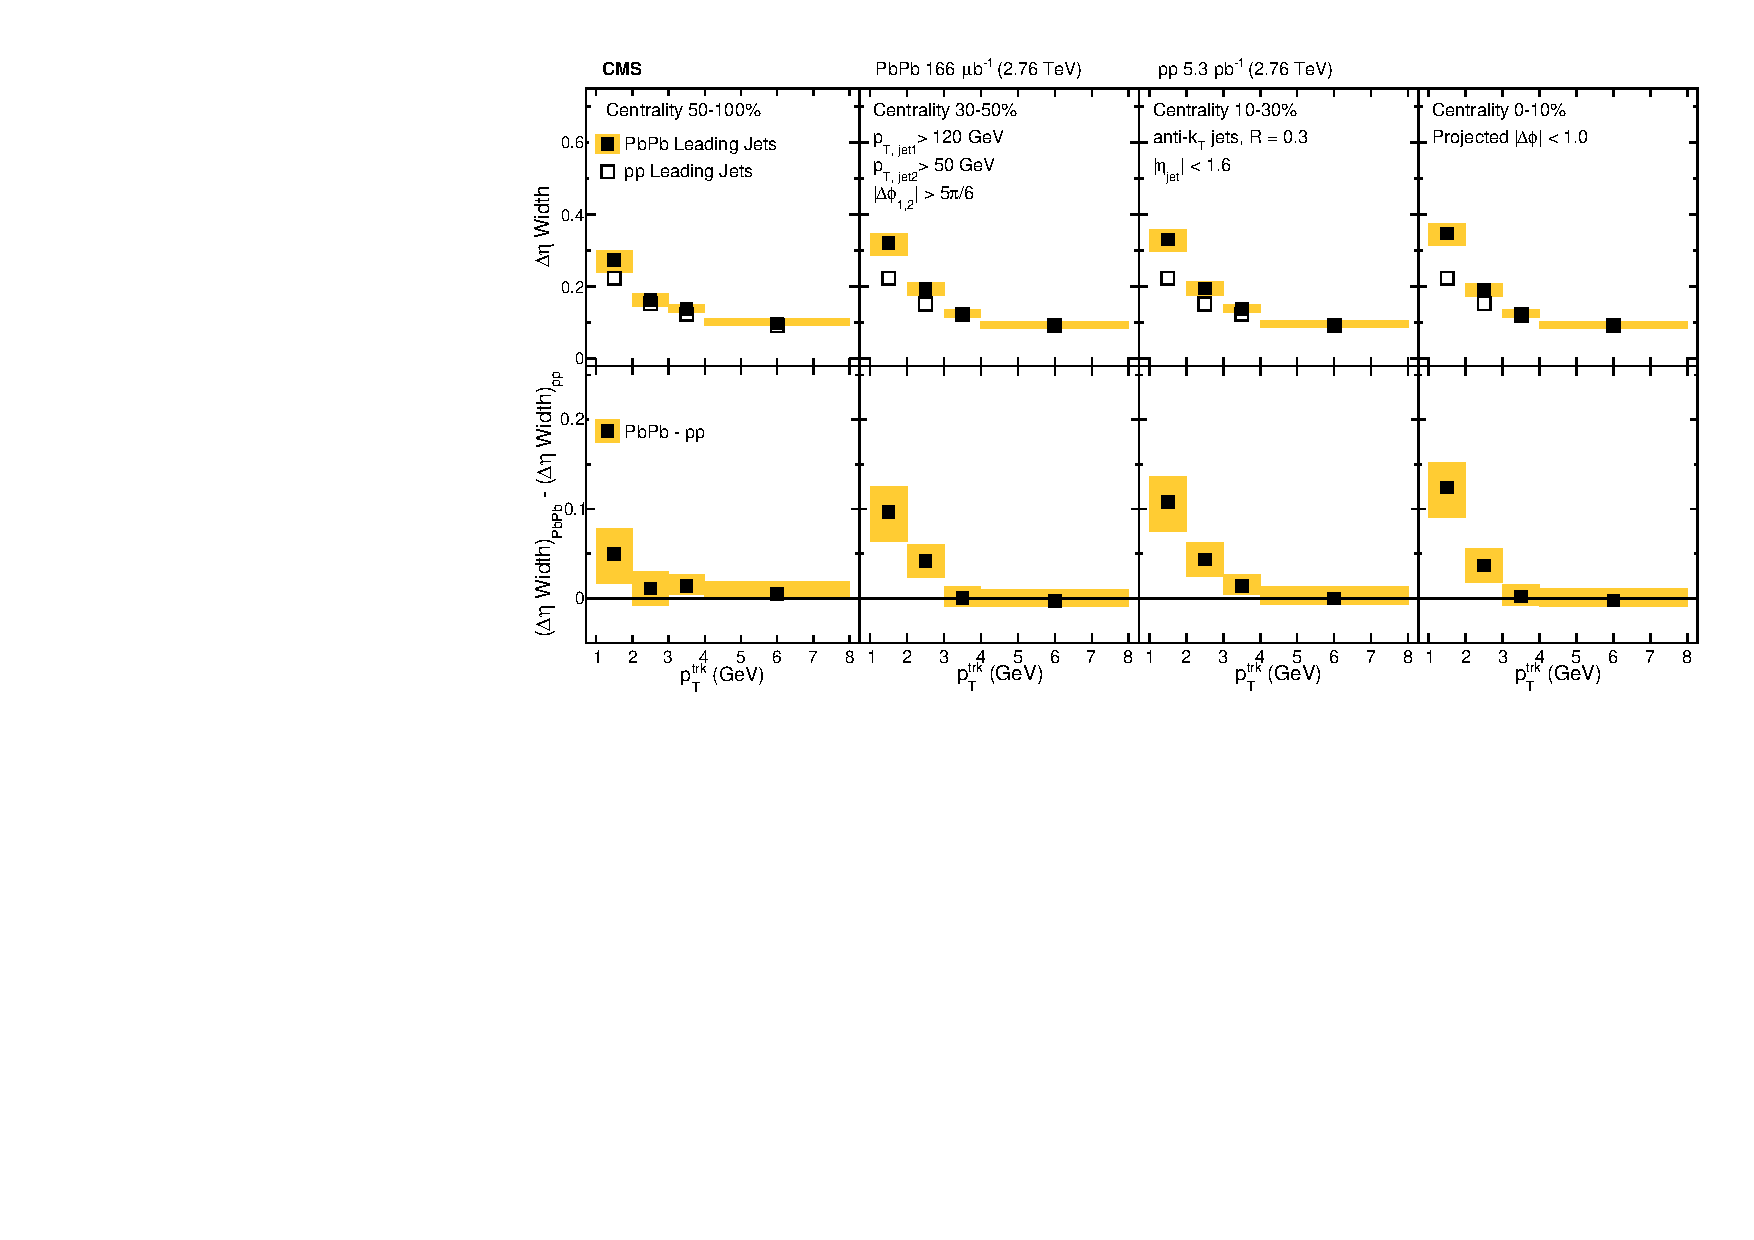
\includegraphics[width=0.99\textwidth]{figures/Results/Width_Eta_Leading.pdf}
\caption[Leading jet $\Delta\eta$ correlation widths as a function of $p_{\rm T}^{\rm trk}$ at 2.76 TeV]{Comparison of the widths in PbPb and pp of the $\protect\Delta\eta$ charged-particle distributions correlated to leading jets with $p_{\rm T, jet1}>$ 120~GeV, as a function of $p_{\rm T}^{\rm trk}$.  The bottom row shows the difference of the widths in PbPb and pp data.  The shaded band corresponds to systematic uncertainty, and statistical uncertainties are smaller than symbol size.}
\label{fig:Width_eta_lead}
\end{center}
\end{figure}

\begin{figure}[hbtp]
\begin{center}
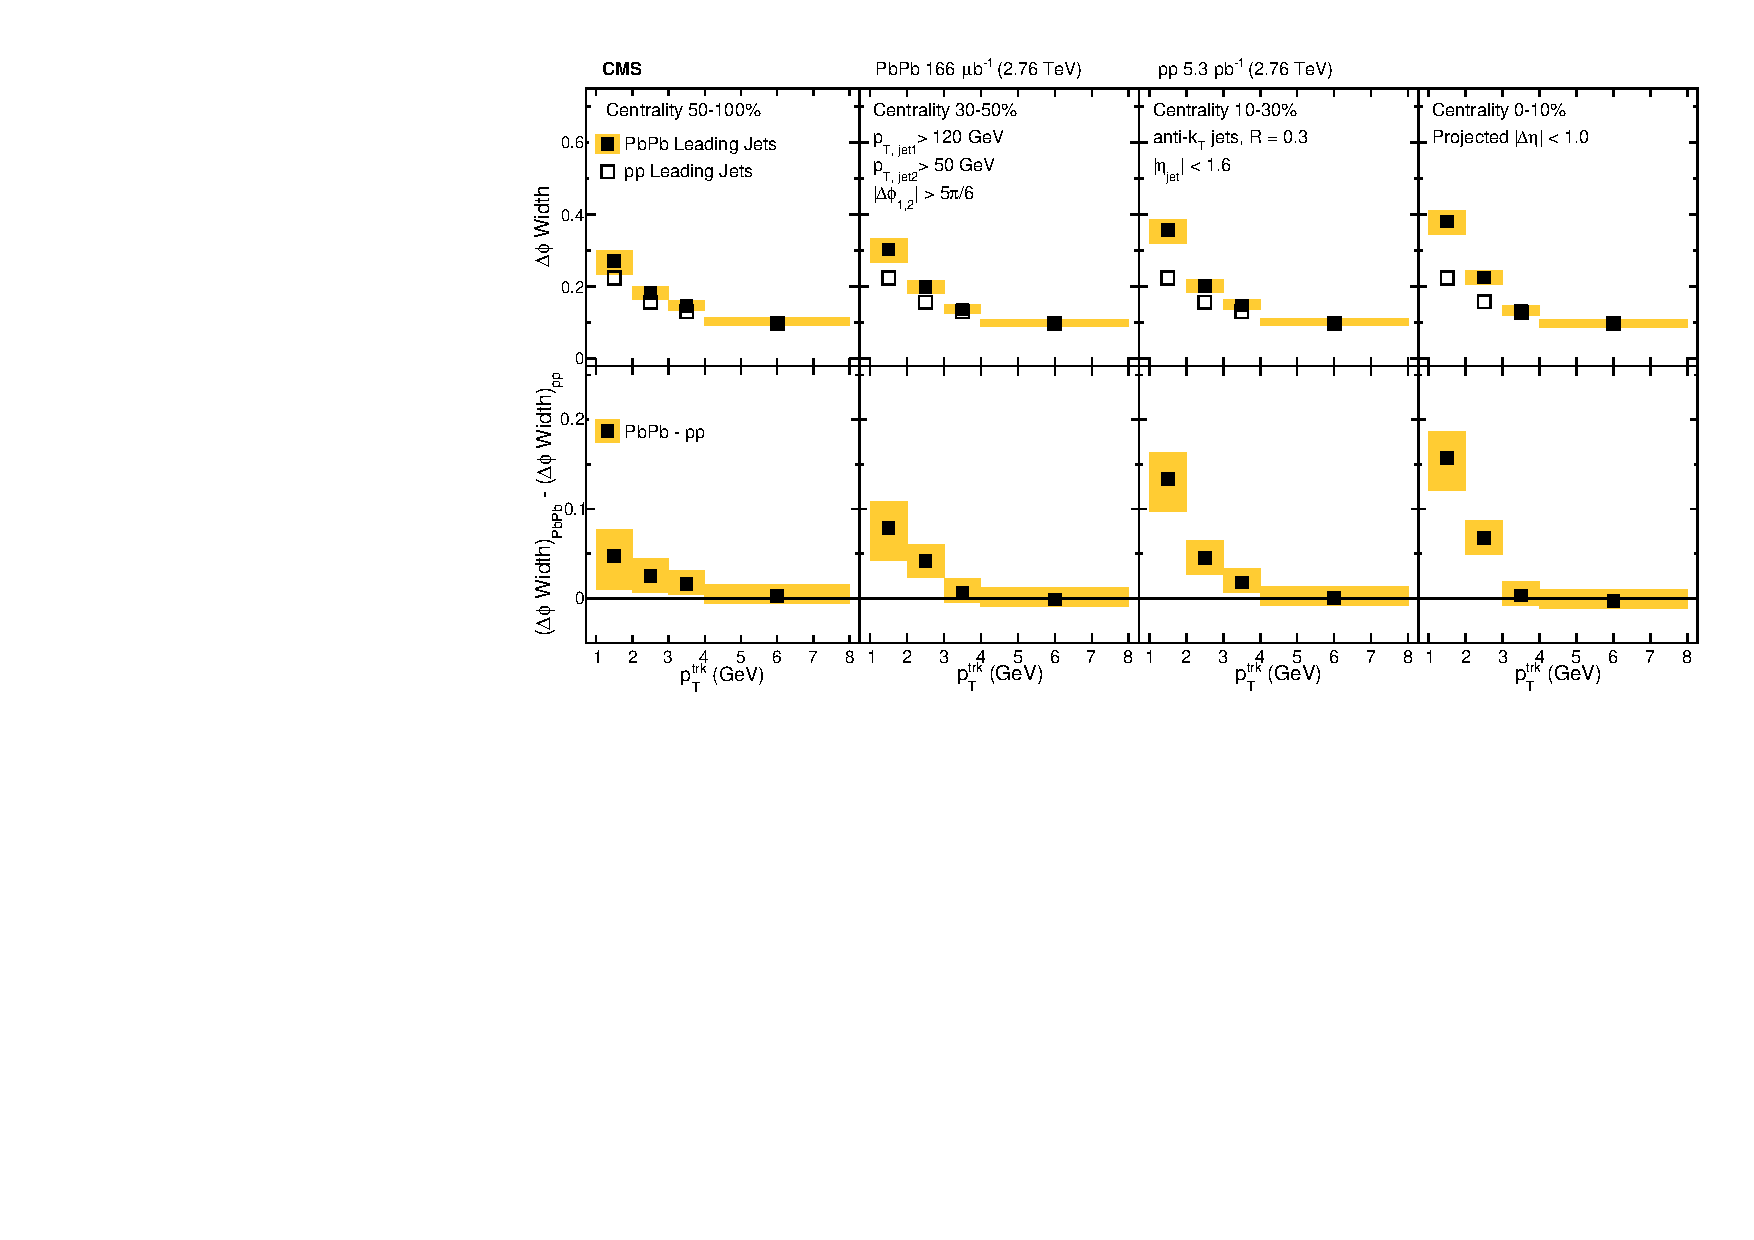
\includegraphics[width=0.99\textwidth]{figures/Results/Width_Phi_Leading.pdf}
\caption[Leading jet $\Delta\phi$ correlation widths as a function of $p_{\rm T}^{\rm trk}$ at 2.76 TeV]{Comparison of the widths in PbPb and pp of the $\protect\Delta\phi$ charged-particle distributions correlated to leading jets with $p_{\rm T, jet1}>$ 120~GeV, as a function of $p_{\rm T}^{\rm trk}$.  The bottom row shows the difference of the widths in PbPb and pp data.  The shaded band corresponds to systematic uncertainty, and statistical uncertainties are smaller than symbol size.}
\label{fig:Width_phi_lead}
\end{center}
\end{figure}

\begin{figure}[hbtp]
\begin{center}
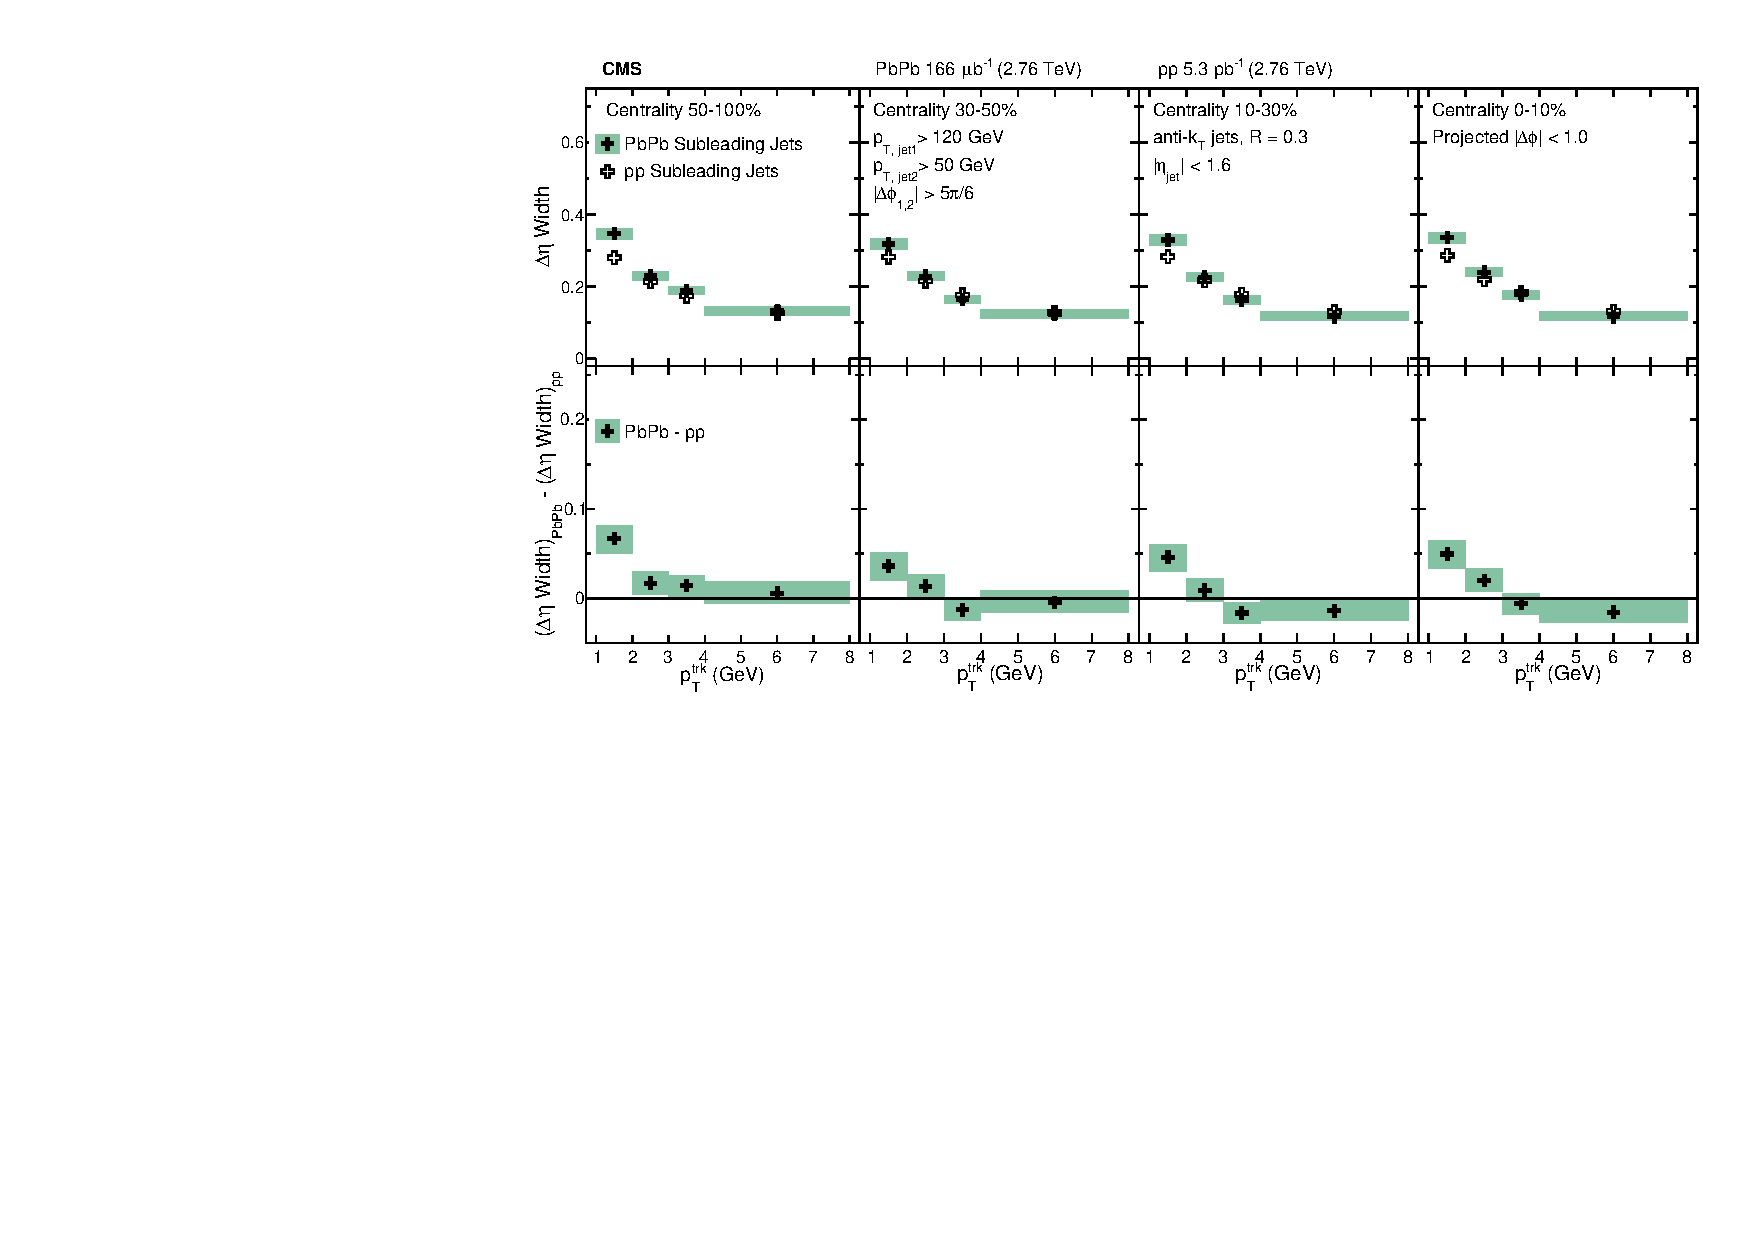
\includegraphics[width=0.99\textwidth]{figures/Results/Width_Eta_SubLeading.pdf}
\caption[Subleading jet $\Delta\eta$ correlation widths as a function of $p_{\rm T}^{\rm trk}$ at 2.76 TeV]{Comparison of the widths in PbPb and pp of the $\protect\Delta\eta$ charged-particle distributions correlated to leading jets with $p_{\rm T, jet2}>$ 50~GeV, as a function of $p_{\rm T}^{\rm trk}$.  The bottom row shows the difference of the widths in PbPb and pp data.  The shaded band corresponds to systematic uncertainty, and statistical uncertainties are smaller than symbol size.}
\label{fig:Width_eta_sub}
\end{center}
\end{figure}

\begin{figure}[hbtp]
\begin{center}
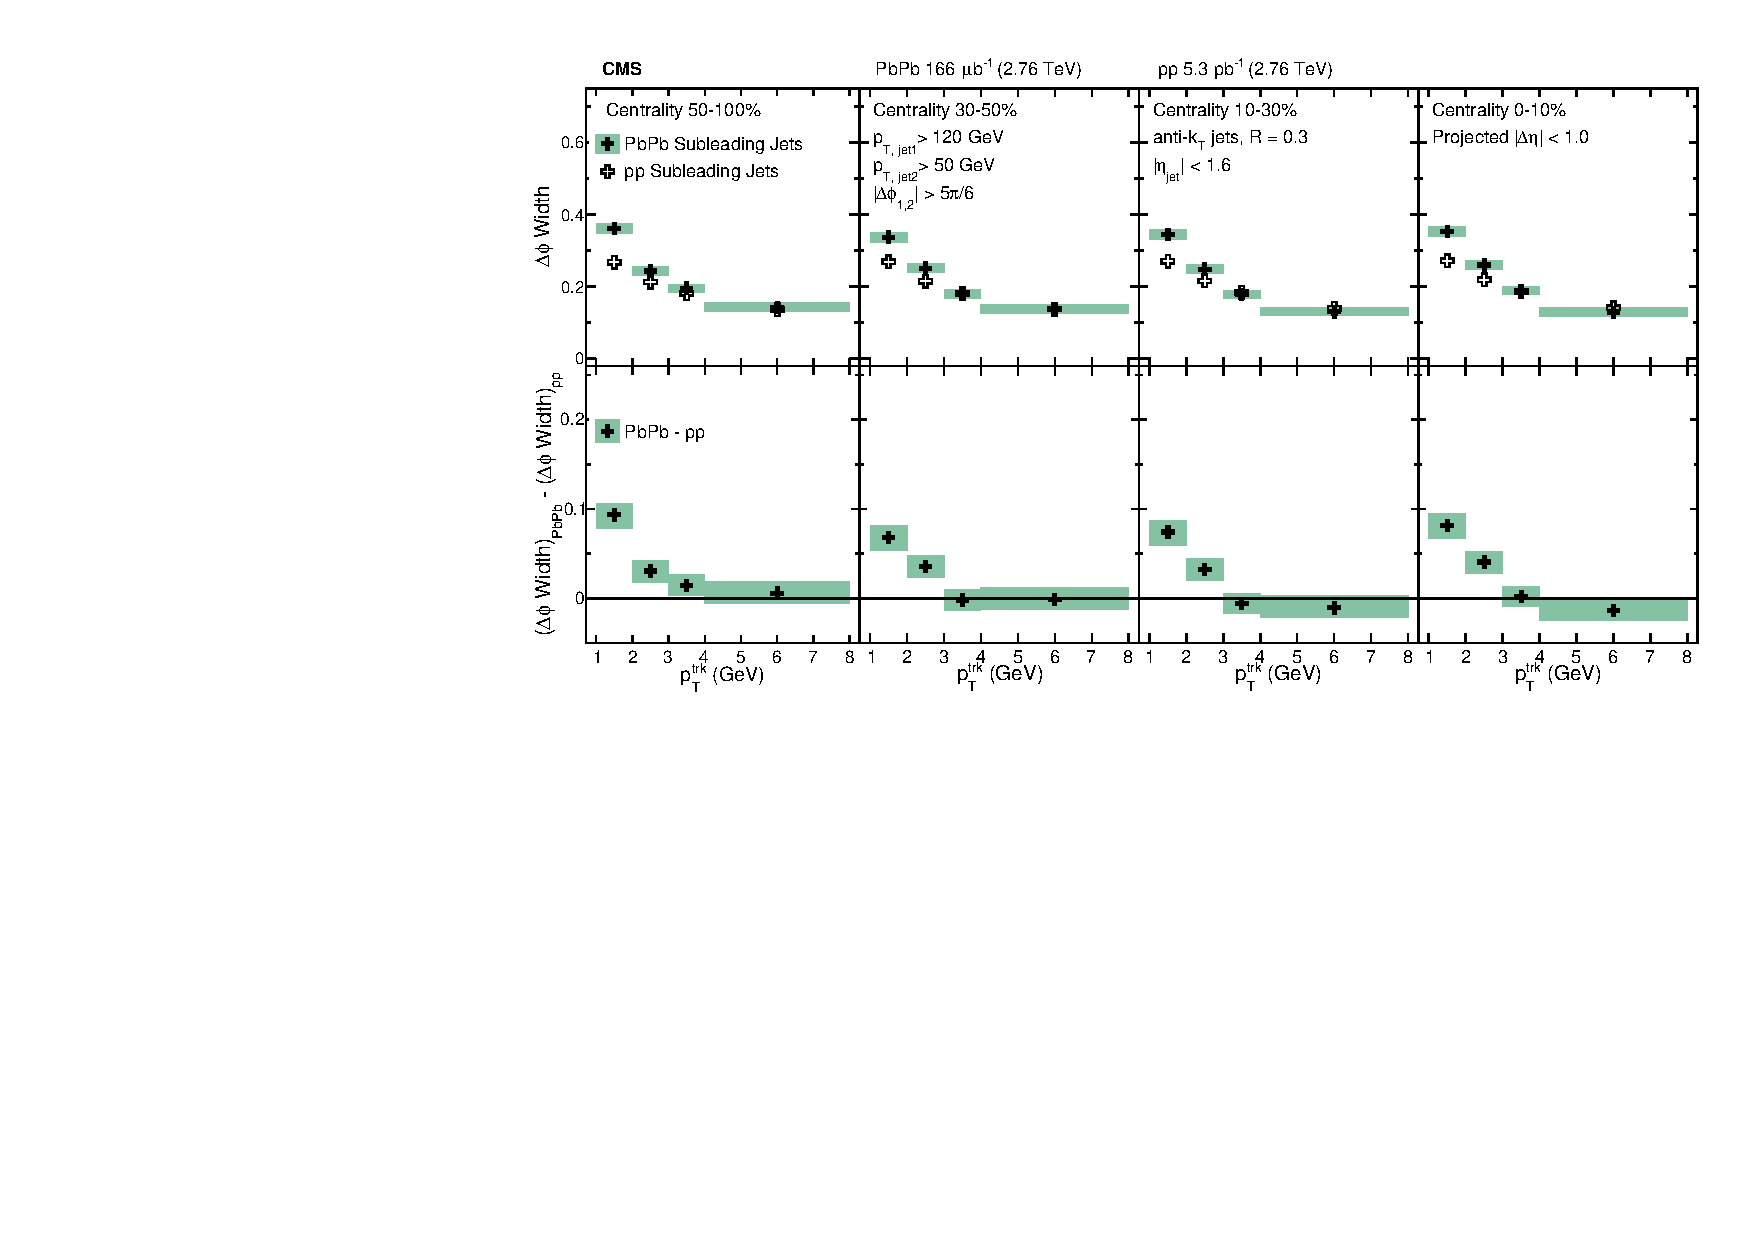
\includegraphics[width=0.99\textwidth]{figures/Results/Width_Phi_SubLeading.pdf}
\caption[Subleading jet $\Delta\phi$ correlation widths as a function of $p_{\rm T}^{\rm trk}$ at 2.76 TeV]{Comparison of the widths in PbPb and pp of the $\protect\Delta\phi$ charged-particle distributions correlated to leading jets with $p_{\rm T, jet2}>$ 50~GeV, as a function of $p_{\rm T}^{\rm trk}$.  The bottom row shows the difference of the widths in PbPb and pp data.  The shaded band corresponds to systematic uncertainty, and statistical uncertainties are smaller than symbol size.}
\label{fig:Width_phi_sub}
\end{center}
\end{figure}



\clearpage


\subsection{Jet shapes at 2.76 TeV and 5.02 TeV}
\label{sec:jet_shapes}

A common observable to characterize and compare the widths of jet peaks is the jet shape $\rho_{\Delta r}$, measuring the fraction of total jet transverse momentum as a function of distance $\Delta r$ from the jet axis.  As discussed in Sec.~\ref{sec:theory_models}, previous CMS measurements of jet shape~\cite{Chatrchyan:2013kwa} have gained particular attention from the theoretical community in efforts to constrain models of jet energy loss.  Jet shape measurements to large angles ($\Delta r = 1$, compared to previous measurements to only $\Delta r = 0.3$) may be obtained from correlation studies, extending measurements to the full range of the jet peak and offering the capability of distinguishing between theoretical predictions based on earlier, more narrow, measurements.  

In the correlation technique, jet shapes are obtained by weighting correlations by $p_{\rm T}^{\rm trk}$, and integrating the resulting (background-subtracted) 2D jet-peak momentum distributions in annuli with radial width $\protect\Delta r = 0.05$, where each has an inner radius of ${\rm r_{a}} = \Delta r - \delta r/2$ and an outer radius of ${\rm r_{b}} = \Delta r + \delta r/2$.  For this measurement, an inclusive high-$p_{\rm T}^{\rm trk}$ bin is included to capture particles with $20 < p_{\rm T}^{\rm trk}< 300 $ GeV.   The resulting transverse momentum profile of the jet is defined as: 

\begin{equation}
{\rm P} (\Delta r) = \frac{1}{\delta r} \frac{1}{N_{\rm jets}} \large{\Sigma_{\rm jets}} \Sigma_{\rm tracks \in (r_{a},r_{b})} p_{\rm T}^{\rm trk}
\end{equation}

\noindent This profile is then normalized to unity within $\protect\Delta r = 1$ to produce the jet shape $\rho(\Delta r)$: 

\begin{equation}
\rho(\Delta r) = \frac{1}{\delta r} \frac{\large{\Sigma_{\rm jets}} \Sigma_{\rm tracks \in (r_{a},r_{b})} p_{\rm T}^{\rm trk}}{\large{\Sigma_{\rm jets}} \Sigma_{\rm tracks} p_{\rm T}^{\rm trk}}
\end{equation}


The top row of Fig.~\ref{fig:jetshape_dr_stacked} presents the inclusive jet transverse momentum profile ${\rm P}(\Delta r)$ in pp and PbPb data at 5.02 TeV, while the middle row shows the jet shape ${\rho}(\Delta r)$, normalized to unity within $\protect\Delta r = 1$.  Here again redistribution of energy from small to large angles from the jet cone is evident in PbPb relative to pp reference, as seen in the dipping then rising trend in the jet shape ratio $\rho(\Delta r)_{\rm PbPb}/\rho(\Delta r)_{\rm pp}$ presented in the bottom row.  

\clearpage

  \begin{figure}[hbt]
    \begin{center}
       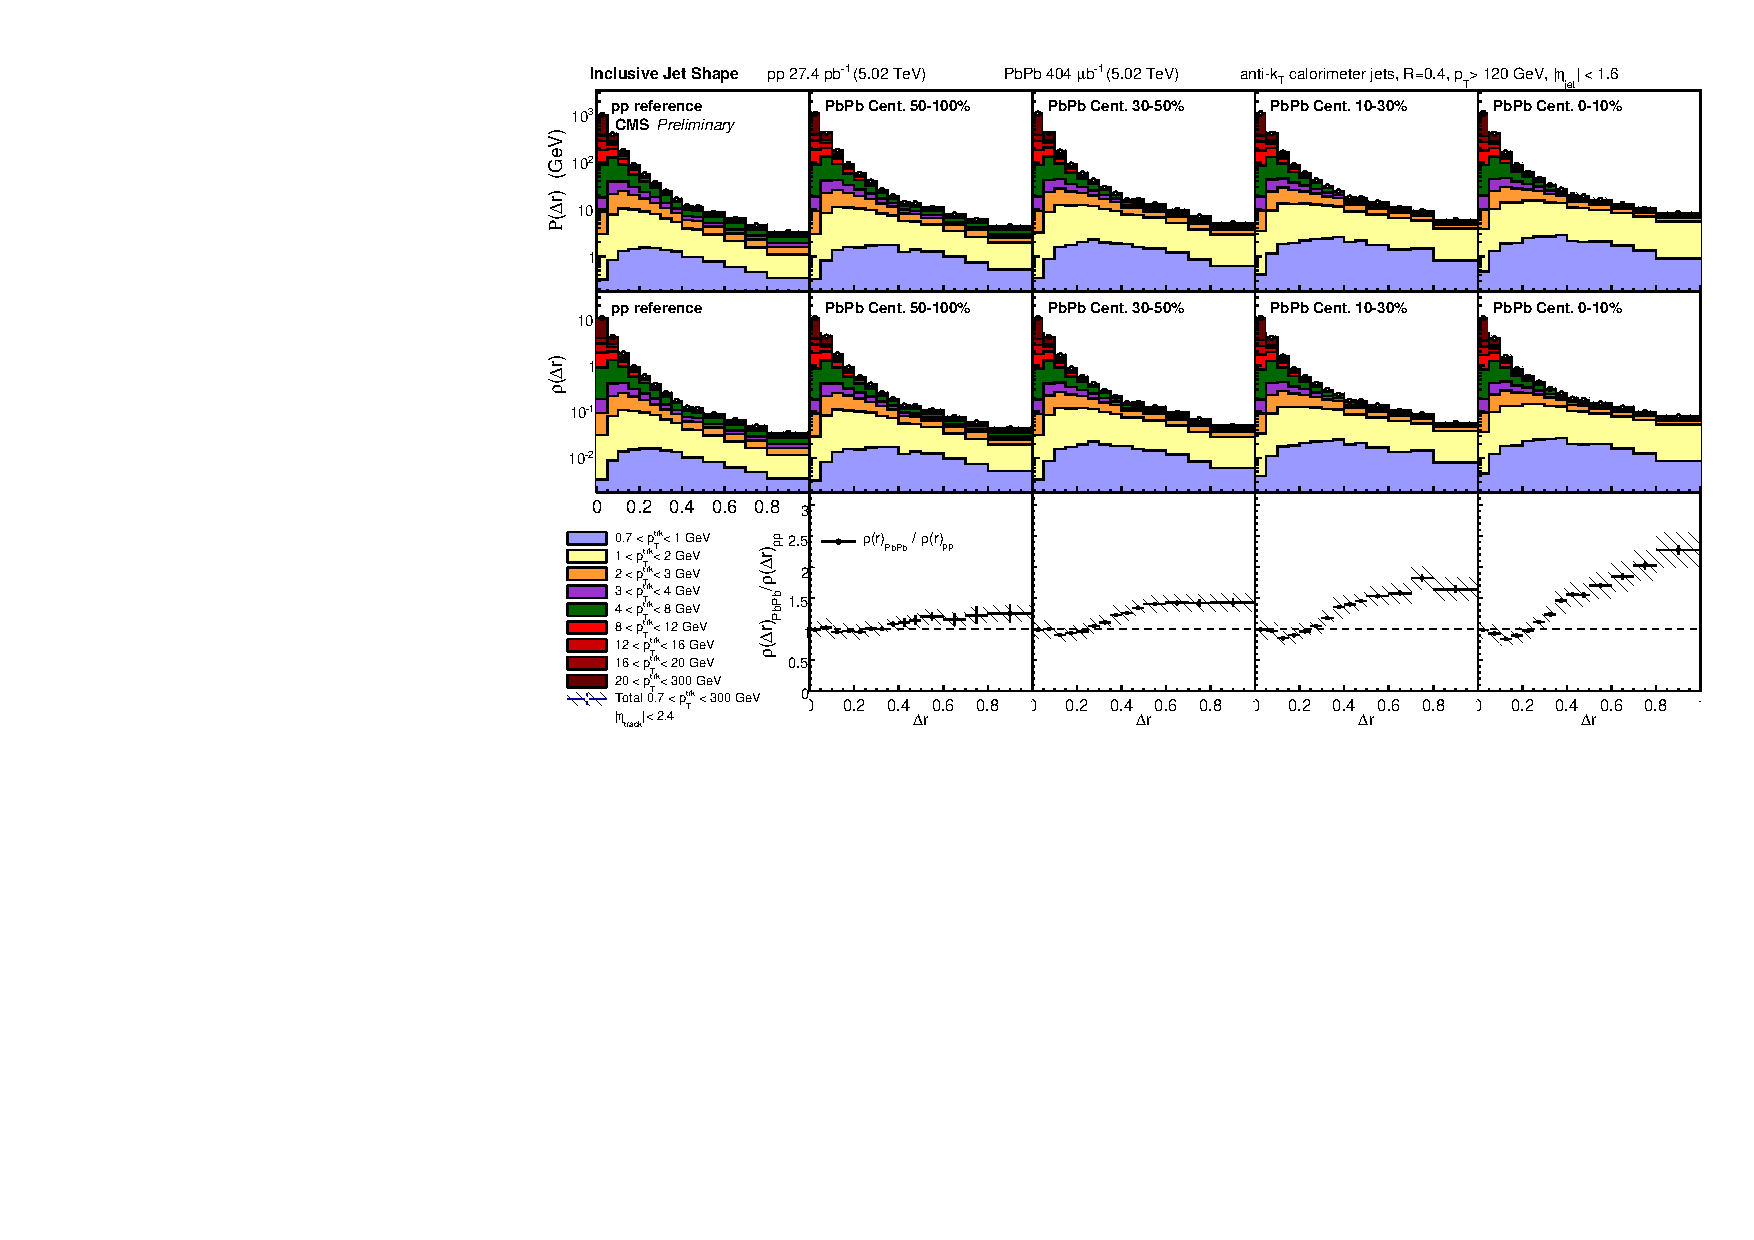
\includegraphics[width=0.99\textwidth]{figures/results/JetShapes_WithHighpT_pTweighted_3Row.pdf}
         \caption[Inclusive jet shape at 5.02 TeV, shown differentially in $p_{\rm T}^{\rm trk}$]{Top row: Transverse momentum profile of inclusive jets ${\rm P}(\Delta r)$ in pp and PbPb data at 5.02 TeV, shown differentially in $p_{\rm T}^{\rm trk}$.  Middle row: jet shapes $\rho(\Delta r)$ (normalized to unity over $\protect\Delta r < 1$) in PbPb and pp. Bottom row:  jet shape ratio $\rho(\Delta r)_{\rm PbPb} / \rho(\Delta r)_{\rm pp}$. Hatched lines on $p_{\rm T}^{\rm trk}$-inclusive points show total systematic uncertainties.}
       \label{fig:jetshape_dr_stacked}
    \end{center}
 \end{figure}


In addition to studies of inclusive jet shapes, it is also interesting to consider the jet shapes and jet shape modifications of leading and subleading jets in dijet events.  These studies are carried out with the same selection of 2.76 TeV dijet events used for the correlation studies presented in~\ref{sec:dijet_corr}.  In this case, for consistency with a previous CMS study measured the jet shape $\rho(\Delta r)$ within the jet cone radius $\Delta r = 0.3$~\cite{Chatrchyan:2013kwa} at 2.76 TeV, these leading and subleading jet shape measurements at 2.76 TeV are normalized to integrate to unity with in the radius $\Delta r < 0.3$.  In Fig.~\ref{fig:JetShape_Leading}, the leading jet shape measured with this correlation technique is compared to the published CMS reference and extend this measurement to $\Delta r = 1$, noting that the leading jet shape is consistent within uncertainties with the previous measurement for an inclusive jet selection of all jets with $p_{\rm T}>100$ GeV.  A new measurement of subleading jet shape in Fig.~\ref{fig:JetShape_SubLeading} is then presented.  As noted in the correlation width measurements discussed in Sec.~\ref{sec:dijet_corr}, subleading jets in pp data are broader than leading jets in pp data.  Therefore, although the PbPb-to-pp $modifications$ are similar for leading and subleading jets, the more steeply falling pp leading jet shape results in a greater \textit{relative} modification shown in the jet shape ratio $\rho_{\rm PbPb}(\Delta r)/\rho_{\rm pp}(\Delta r)$ for leading than for subleading jets.  Similarly, when comparing jet shape measurements at 2.76 TeV to those at 5.02 TeV, it is relevant to note hat the pp reference is broader at 5.02 TeV than at 2.76 TeV, likely due to the greater fraction of gluon versus quark jets that pass the kinematic selections of the analysis at the higher center-of-mass energy.  


\begin{figure}[h!]
\begin{center} 
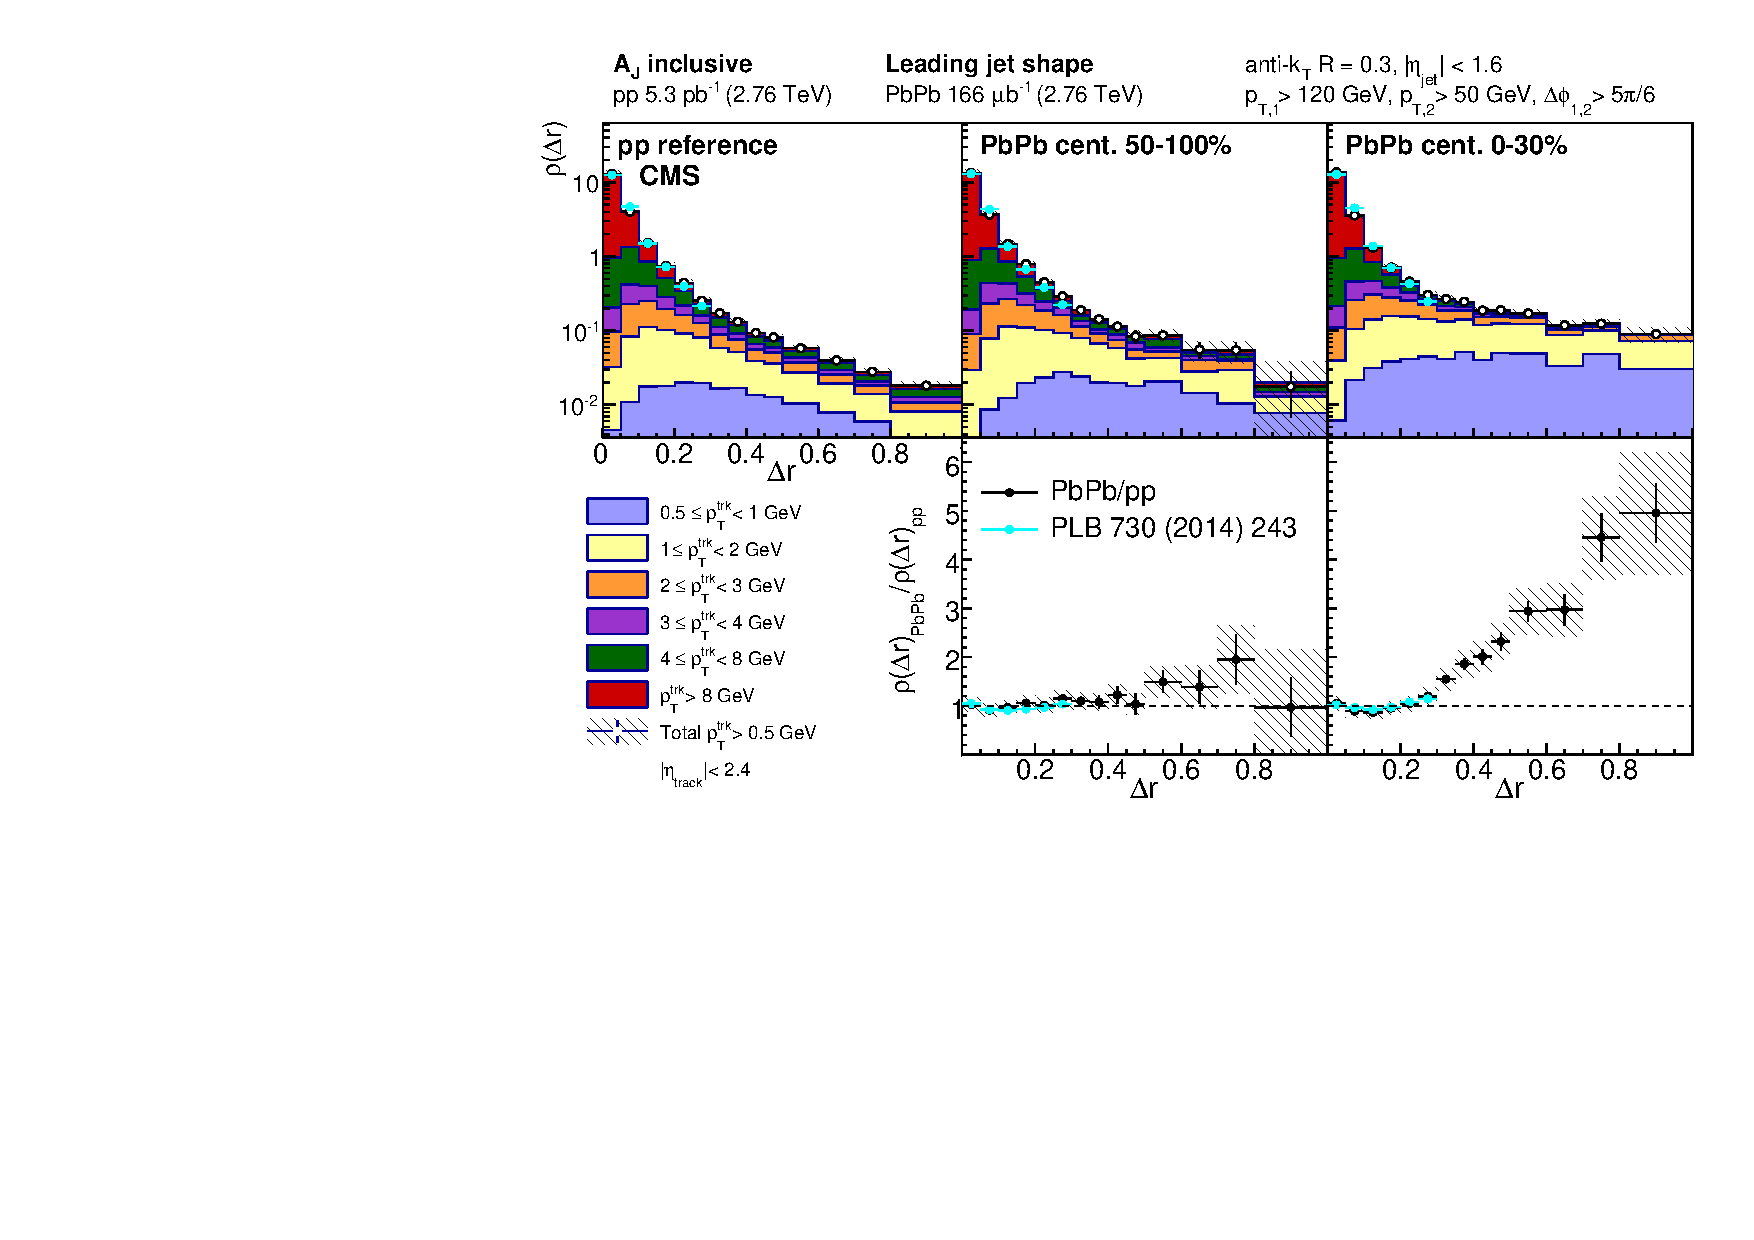
\includegraphics[width=0.99\textwidth]{figures/Results/JetShapes_WithHighpT_PAS.pdf}
\caption[Leading jet shape at 2.76 TeV, shown differentially in $p_{\rm T}^{\rm trk}$]{Top row:  leading jet shape $\rho(\Delta r)$ for pp reference and central and peripheral PbPb data, shown for all tracks with $p_{\rm T}^{\rm trk} > 0.5$ GeV and decomposed by track transverse momentum.  Shapes are normalized to unity over the region $r<0.3$ for consistency with the published reference shown (Ref.~\cite{Chatrchyan:2013kwa}).  Bottom row:  leading jet shape ratio $\rho(\Delta r)_{\rm PbPb}/\rho(\Delta r)_{\rm pp}$, again with published reference.  }
\label{fig:JetShape_Leading} 
\end{center} 
\end{figure} 



\begin{figure}[h!]
\begin{center} 
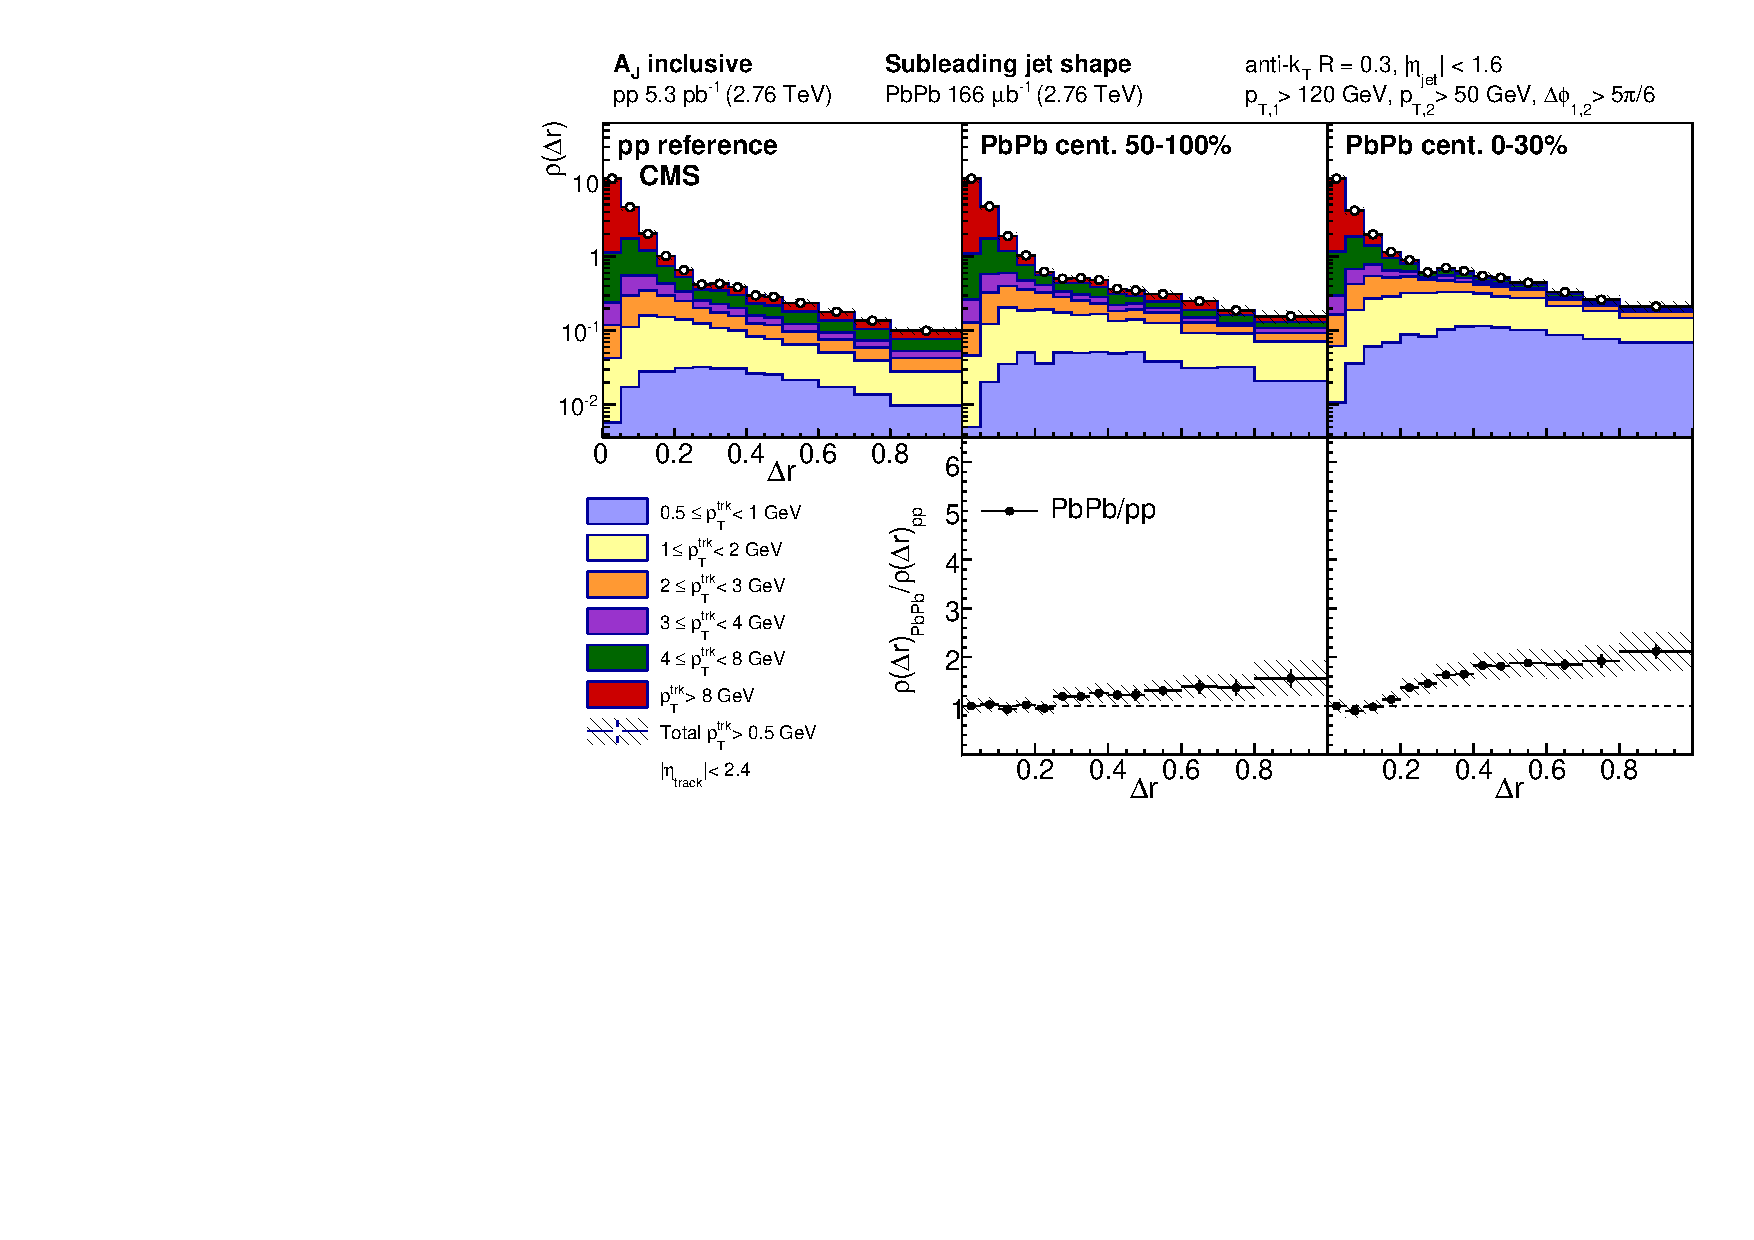
\includegraphics[width=0.99\textwidth]{figures/Results/JetShapes_SubLeading_WithHighpT_PAS.pdf}
\caption[Subleading jet shape at 2.76 TeV, shown differentially in $p_{\rm T}^{\rm trk}$]{Top row:  subleading jet shape $\rho(\Delta r)$ for pp reference and central and peripheral PbPb data, shown for all tracks with $p_{\rm T}> 0.5$ GeV and decomposed by track transverse momentum, normalized to unity over the region $\Delta r<0.3$ Bottom row:  subleading jet shape ratio $\rho(\Delta r)_{\rm PbPb}/\rho(\Delta r)_{\rm pp}$. }
\label{fig:JetShape_SubLeading} 
\end{center} 
\end{figure} 



\clearpage



\subsection{Decomposition of hemisphere momentum balance in dijet events at 2.76 TeV}
\label{sec:dijet_mpt}

The dijet results at 2.76 TeV presented in this analysis are complimented by other CMS measurements conducted on the same data using the ``missing-$p_{\rm T}$'' hemisphere momentum balance method presneted in Ref.~\cite{HIN_2014_010} and discussed in Secs.~\ref{sec:theory_jets} and~\ref{sec:theory_models}.  In this analysis, a ``dijet'' axis is constructed by averaging the leading jet and subleading jet axes (these are separated by $\Delta\phi_{\rm 1,2} = \pi$ on average, but are not necessarily parallel in each event due to 3-jet events) to construct a dijet axis, dividing the event into leading and subleading hemispheres with respect to this axis, and comparing the hemisphere-wide distributions of $p_{\rm T}^{\rm trk}$ (projected, in this case, onto the combined dijet axis) to obtain the subleading-to-leading balancing distribution as a function of distance from the dijet axis $\Delta r$.  The jet track correlation technique may be used to obtain this same measurement (comparing subleading-to-leading distributions on average rather than event-by-event, and making use of the fact that the subleading and leading jet axes are \textit{on average} perfectly back-to-back).  When this cross-check is performed \textit{without background subtraction}, the two techniques yield consistent results, despite methodological differences and differences in jet-$\eta$ cuts.  This hemisphere-wide missing-$p_{\rm T}$ technique is also used to extract differences in total particle yields between the leading and subleading hemispheres, and shows an average excess of 4-5 particles with $p_{\rm T}^{\rm trk}$ in the subleading hemisphere compared to the leading hemisphere~\cite{HIN_2014_010}.  In the dijet correlation studies presented in this analysis \textit{with background subtraction}, however, only approximately 2 additional particles were found correlated to the subleading jet peak compared to the leading jet peak, as shown in Sec.~\ref{sec:dijet_corr}.  This apparent difference motivates a detailed examination and decomposition of the distribution of $p_{\rm T}^{\rm trk}$ in dijet events in order to consider contributions to the hemisphere-wide momentum balance from both the leading and subleading jet peaks, and from the long-range correlated underlying event.  

For this investigation, the dijet samples of 2.76 TeV PbPb and pp data are each divided based on asymmetry paramter $A_{\rm J}$ to further illuminate quenching effects and to decompose the contributions to the hemisphere $p_{\rm T}^{\rm trk}$ balance studied in Ref.~~\cite{HIN_2014_010}:  a balanced sample with $A_{\rm J} < 0.22$, and an ``unbalanced'' sample with $A_{\rm J} > 0.22$.  Transverse momenum distributions for each sample are constructed in $\Delta\eta--\Delta\phi$ for each sample, and are corrected for pair-acceptance effects.  Like all particle density and $p_{\rm T}^{\rm trk}$ correlations studied in this analysis, these show jet peaks on an underlying event that shows significant $\Delta\phi$ correlations but is flat in $\Delta\eta$.  Correlations are therefore projected into $\Delta\phi$ for further study in order to preserve this underlying event structure.  Studies will begin by considering the hemisphere-wide ``missing-$p_{\rm T}$'' distribution as a function of $\Delta\phi$, and will then decompose this distribution into jet peak and underlying event contributions, and finally consider the relative contributions from jet peaks and from the underlying event to the overall hemisphere $p_{\rm T}^{\rm trk}$ balance for balanced and unbalanced dijets.   

Figures~\ref{fig:MpT_nobkgsub_Aj0_Aj22} and~\ref{fig:MpT_nobkgsub_Aj22_Aj75} present the hemisphere-wide balancing distribution of transverse momentum around the subleading versus the leading jet for balanced and unbalanced dijets respectively.  For both selections, a wide excess of soft particles in the subleading versus leading hemisphere in central PbPb collisions relative to pp reference is evident, reflecting the greater quenching of the subleading jet.  In the unbalanced selection, as required by momentum conservation, the signal is enhanced in both pp and PbPb data:  in pp a large excess of particles with $p_{\rm T}>3$ GeV long-range is present on the subleading side, compensating for the lower momentum of the highest-$p_{\rm T}$ particles in the jet itself.  In peripheral PbPb data the distribution is quite similar to pp reference, while in central PbPb data this balancing distribution consists mostly of soft particles $p_{\rm T}<3$ GeV, consistent with the findings of a previous CMS study~\cite{HIN_2014_010}.  To better demonstrate these medium modifications, the difference in yield between PbPb and pp collisions is shown in the bottom panels of Fig.~\ref{fig:MpT_nobkgsub_Aj0_Aj22} and Fig.~\ref{fig:MpT_nobkgsub_Aj22_Aj75}.

\begin{figure}[h!]
\begin{center} 
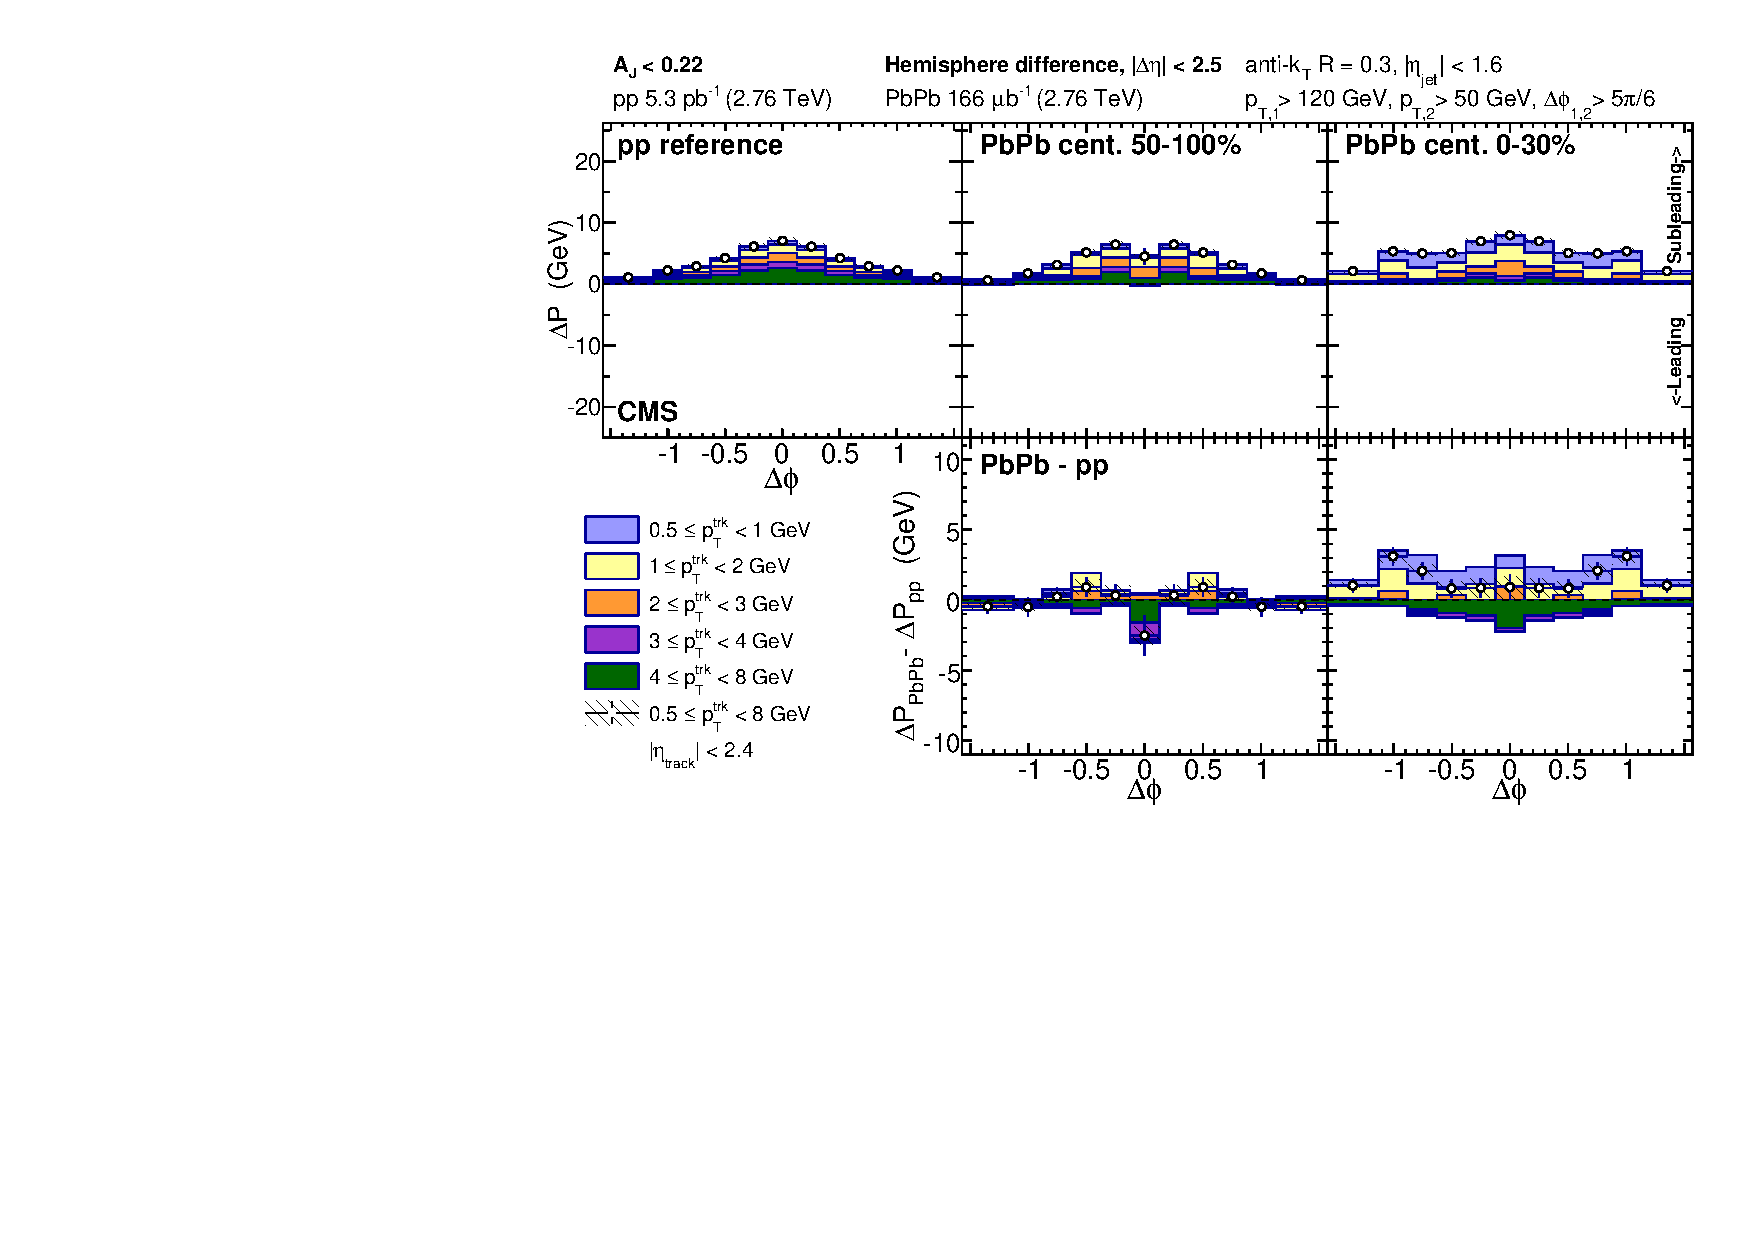
\includegraphics[width=0.99\textwidth]{figures/Results/Missing_pT_NoBkgSub_Aj0_Aj22.pdf}
\caption[Dijet subleading-to-leading hemisphere momentum balance for balanced dijets]{Top row:  total hemisphere distribution in $\protect\Delta\phi$ of excess tranverse momentum about the subleading relative to the leading jet for balanced dijets with $A_{\rm J} < 0.22$, shown differentially by track transverse momentum for pp reference, peripheral PbPb, and central PbPb data.  Bottom row:  PbPb--pp difference in these $\protect\Delta\phi$ momentum distributions.}
\label{fig:MpT_nobkgsub_Aj0_Aj22} 
\end{center} 
\end{figure} 

\begin{figure}[hbt]
\begin{center} 
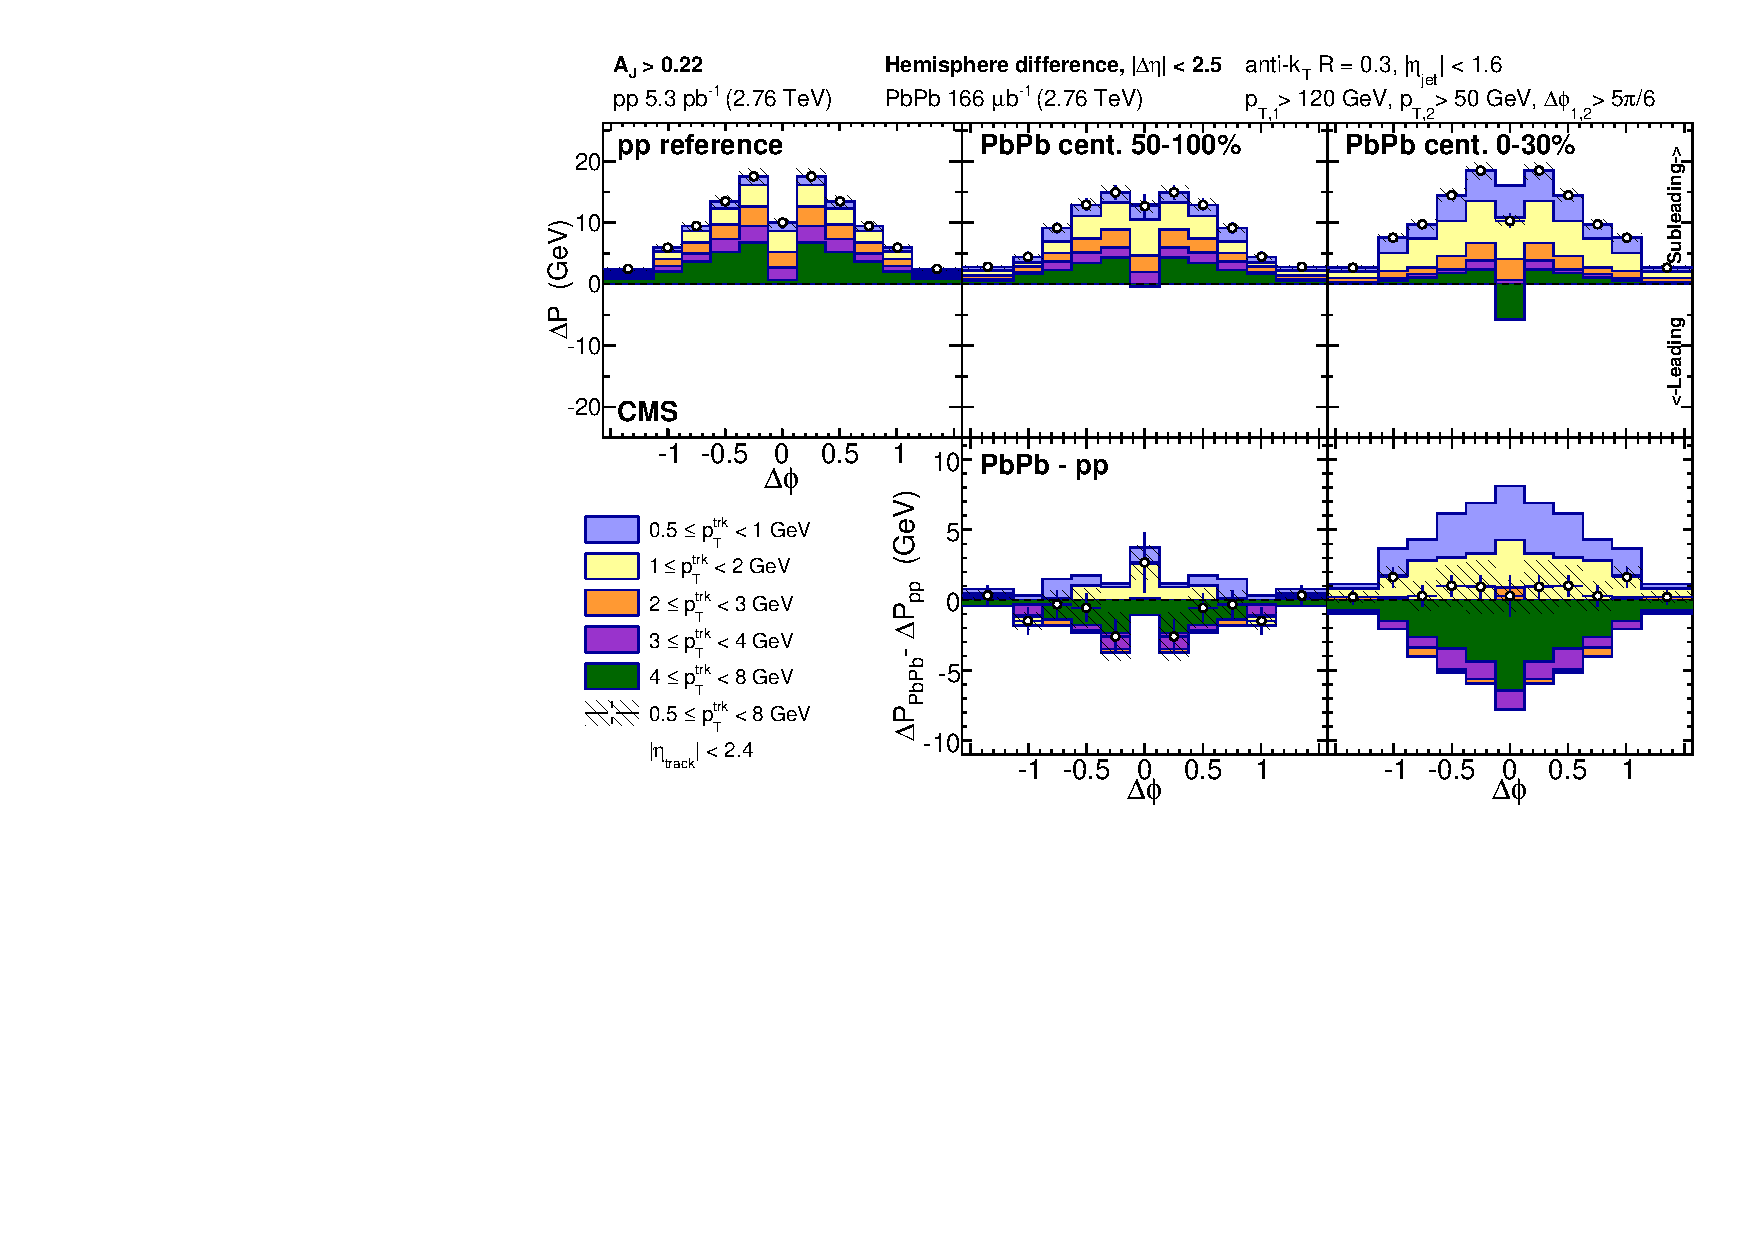
\includegraphics[width=0.99\textwidth]{figures/Results/Missing_pT_NoBkgSub_Aj22_Aj75.pdf}
\caption[Dijet subleading-to-leading hemisphere momentum balance for unbalanced dijets]{Top row:  total hemisphere distribution in $\protect\Delta\phi$ of excess tranverse momentum about the subleading relative to the leading jet for balanced dijets with $A_{\rm J} > 0.22$, shown differentially by track transverse momentum for pp reference, peripheral PbPb, and central PbPb data.  Bottom row:  PbPb--pp difference in these $\protect\Delta\phi$ momentum distributions.}
\label{fig:MpT_nobkgsub_Aj22_Aj75} 
\end{center} 
\end{figure} 

To better understand the redistribution of transverse momentum within the QGP, the distributions are then separated into three components as discussed above:  the gaussian-like peaks about the leading and subleading jet axes, plus a component accounting for overall subleading-to-leading asymmetry in the $\protect\Delta\phi$-correlated long-range underlying event (measured in the region $1.5<|\Delta\eta|<2.5$.  In Fig.~\ref{fig:MpT_jetrelated_Aj0_Aj22} and Fig.~\ref{fig:MpT_jetrelated_Aj22_Aj75}, the jet peak components are shown for balanced and unbalanced jets respectively, presenting subleading results positive and leading results negative (in line with the hemisphere difference measurements in Fig.~\ref{fig:MpT_nobkgsub_Aj22_Aj75} and Fig.~\ref{fig:MpT_nobkgsub_Aj0_Aj22}).  Jet peak distributions after decomposition are projected over the full range $|\Delta\eta|<2.5$, again for consistency with the hemisphere difference measurements.  The top row of each panel first shows the overall distribution of momentum carried by particles with $p_{\rm T} < 8$ GeV on about the jet peak.  The middle two panels then assess modifications to the subleading and leading jets, respectively.  Here there is evidence of quenching to both the subleading and the leading jet in central PbPb collisions relative to pp reference, with an excess of low-$p_{\rm T}^{\rm trk}$ particles correlated to the jet axis in both the balanced and unbalanced dijet selections, as observed in the charged particle density studies presented in Sec.~\ref{sec:dijet_corr}.  In unbalanced dijets this enhancement of soft-$p_{\rm T}^{\rm trk}$ particles turns into a depletion at higher-$p_{\rm T}^{\rm trk}$, and is greater on the subleading than the leading side.  To compare between hemispheres and assess the jet peak contribution to the overall hemisphere momentum balance, the double difference PbPb--pp, subleading--leading is presented in the bottom panel.  Here it is evident that the low-$p_{\rm T}^{\rm trk}$ excess in central PbPb collisions is larger on the subleading than the leading side of the dijet system, but larger subleading-to-leading excess only accounts for only a portion of the total momentum redistribution in unbalanced dijet events.

\begin{figure}[hbt]
\begin{center} 
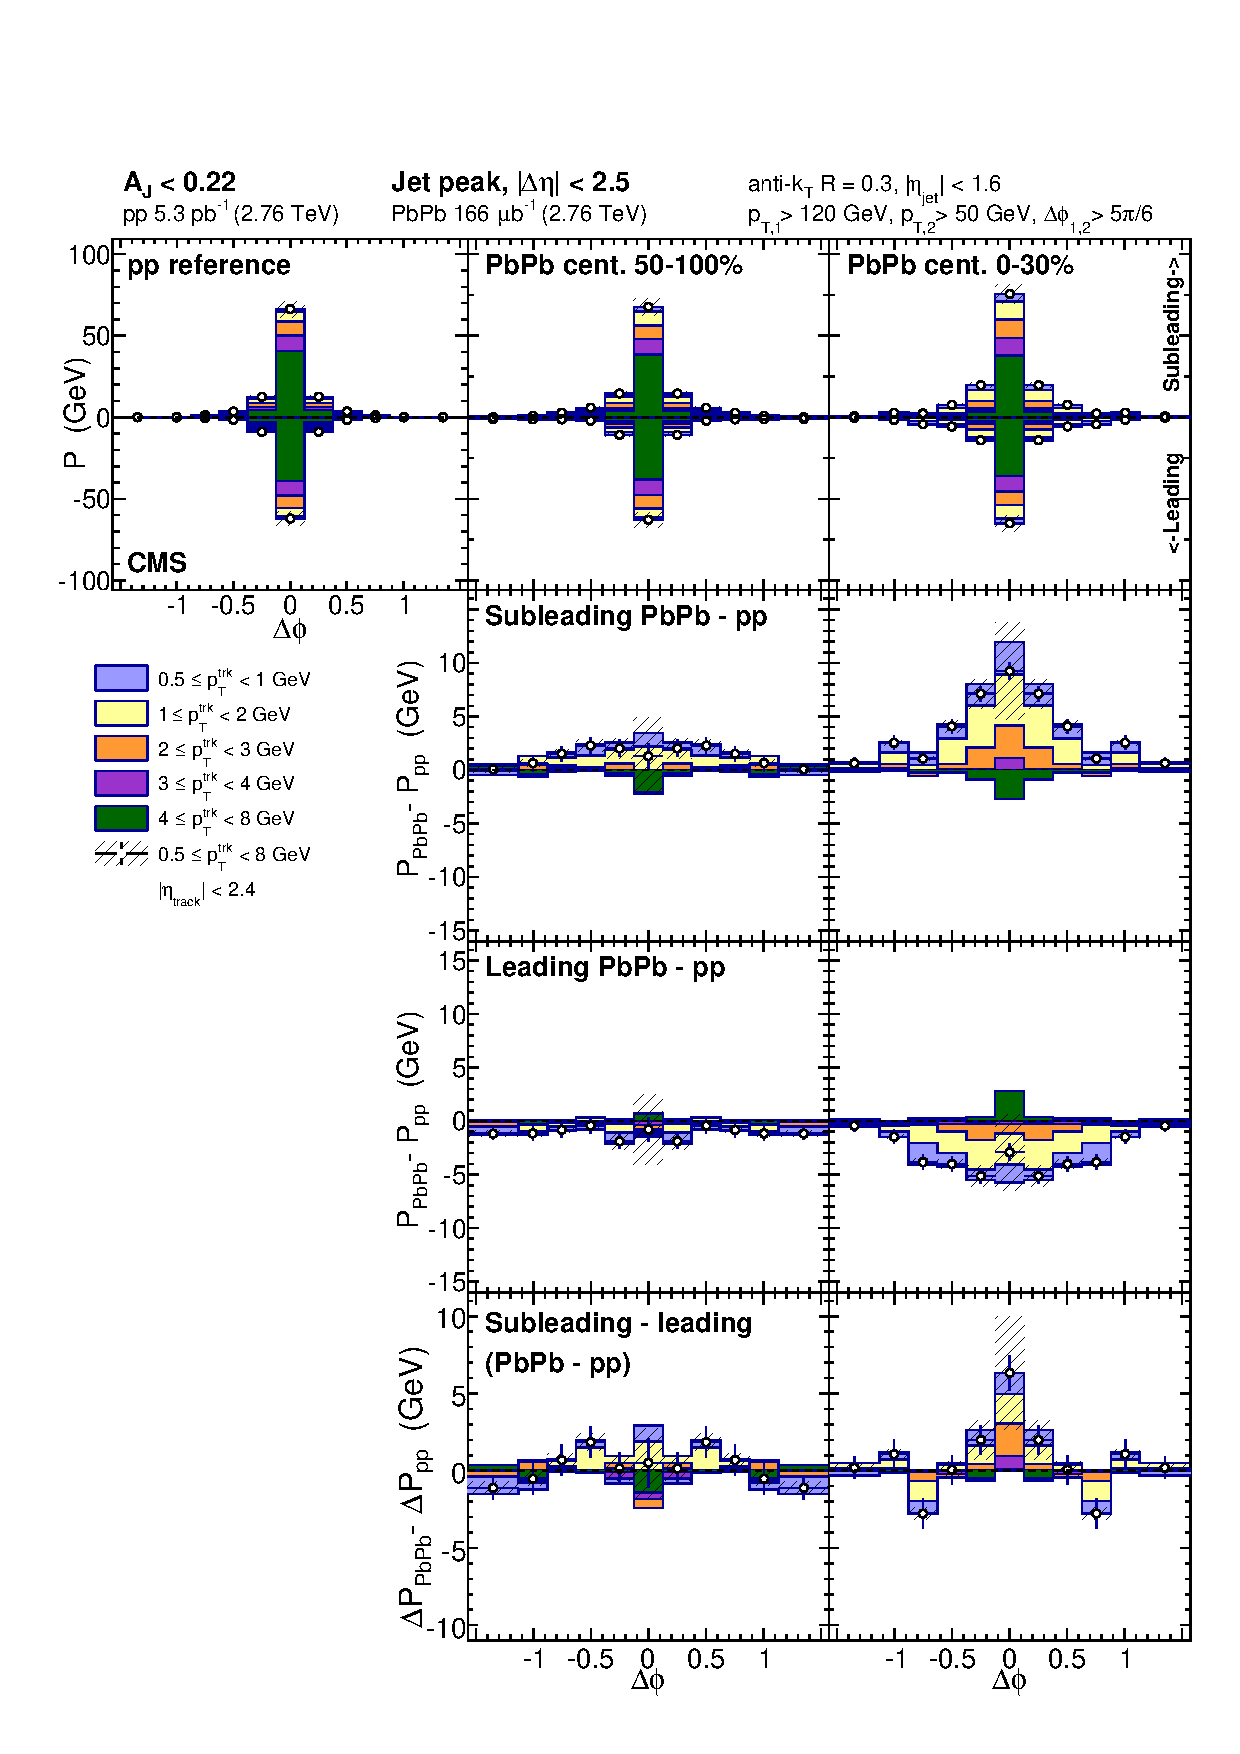
\includegraphics[width=0.99\textwidth]{figures/Results/Missing_pT_JetRelated_Aj0_Aj22.pdf}
\caption[Jet peak subleading-to-leading momentum balance for balanced dijets]{Top row:  jet-peak (long-range subtracted) distribution in $\protect\Delta\phi$ of tranverse momentum about the subleading (plotted positive) and leading (plotted negative) jets for balanced dijets with $A_{\rm J} < 0.22$.  Middle rows:  PbPb--pp momentum distribution differences for subleading and leading jets.  Bottom row:  PbPb--pp, subleading--leading double difference in these $\protect\Delta\phi$ momentum distributions.}
\label{fig:MpT_jetrelated_Aj0_Aj22} 
\end{center} 
\end{figure} 

\begin{figure}[hbt]
\begin{center} 
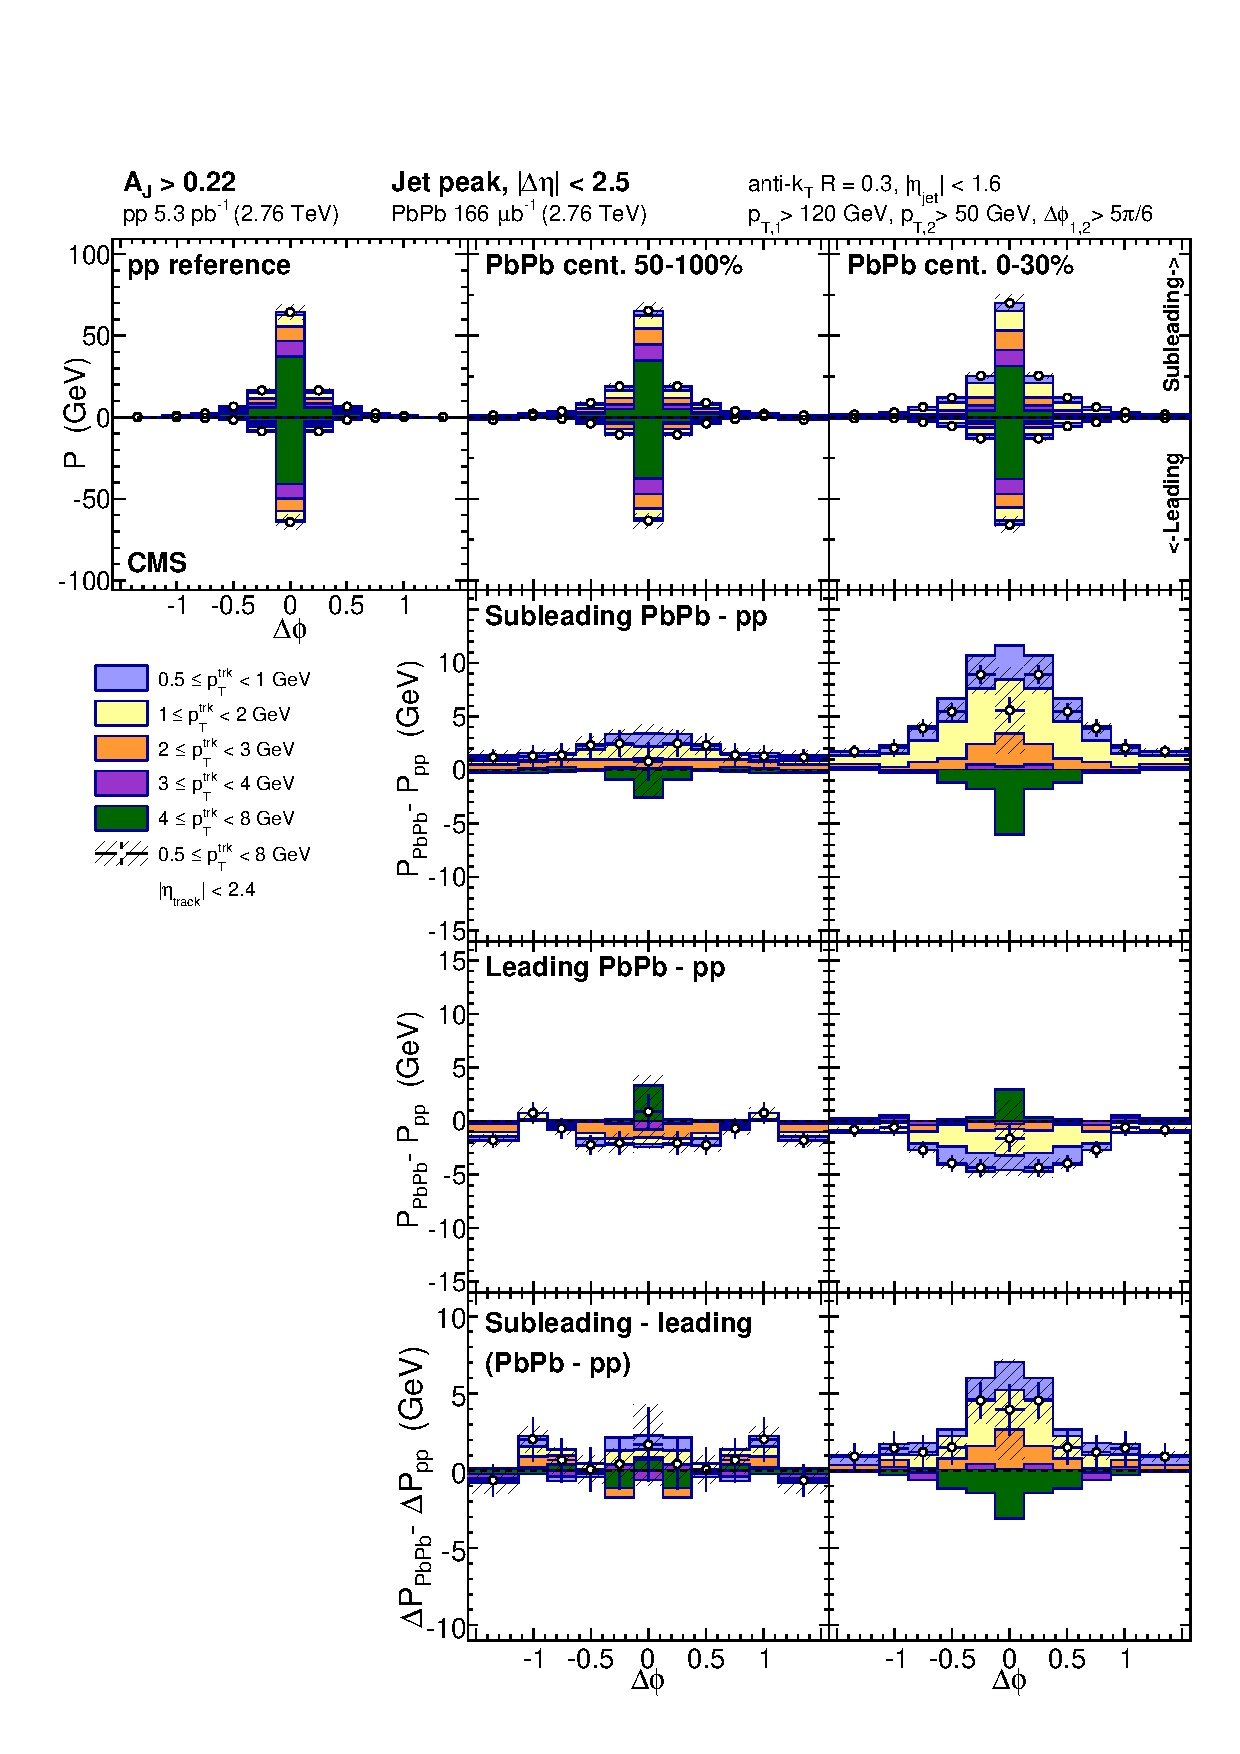
\includegraphics[width=0.99\textwidth]{figures/Results/Missing_pT_JetRelated_Aj22_Aj75.pdf}
\caption[Jet peak subleading-to-leading momentum balance for unbalanced dijets]{Top row:  jet-peak (long-range subtracted) distribution in $\protect\Delta\phi$ of tranverse momentum about the subleading (plotted positive) and leading (plotted negative) jets for balanced dijets with $A_{\rm J} > 0.22$.  Middle rows:  PbPb--pp momentum distribution differences for subleading and leading jets.  Bottom row:  PbPb--pp, subleading--leading double difference in these $\protect\Delta\phi$ momentum distributions.}
\label{fig:MpT_jetrelated_Aj22_Aj75} 
\end{center} 
\end{figure} 

\clearpage

These jet-related studies are complemented by an analysis of the long-range subleading to leading asymmetry, presented in Fig.~\ref{fig:MpT_longrange_Aj0_Aj22}  and Fig.~\ref{fig:MpT_longrange_Aj22_Aj75} for balanced and unbalanced jets respectively.  The long-range correlated background in balanced dijet events is symmetric in pp and peripheral PbPb data, while in central PbPb data there is a small excess of low-$p_{\rm T}^{\rm trk}$ particles.  In unbalanced dijets, however, there is significant asymmetry already in pp reference, with a large correlated excess of particles in all $p_{\rm T}$ classes less than 8 GeV on the subleading relative to leading side of the underlying event.  This asymmetry reflects the presence of other hard-scattering products in the subleading hemisphere dijet event, as required by momentum conservation when selecting asymmetric dijets in vacuum-like collisions.  In the presence of the strongly interacting medium;  however, this underlying event asymmetry in asymmetric dijet events changes notably.  In peripheral PbPb collisions there is already some depletion of momentum carried by high-$p_{\rm T}^{\rm trk}$ particles, and in central pp collisions subleading-to-leading underlying event excesses with $p_{\rm T}^{\rm trk} > 2$ GeV vanish nearly completely.  To assess the contribution of this long-range asymmetry to the total hemisphere imbalance, the double difference PbPb--pp, subleading--leading is plotted on the bottom panel as for (and on the same scale as) the double difference shown for the jet peaks.  To assess the overall hemisphere momentum balance attributed to this long-range asymmetry, the hemisphere integral ($|\Delta\phi|<\pi/2$ and $|\Delta\eta|<2.5$) is presented in Fig.~\ref{fig:Integral_Longrange} for balanced versus unbalanced dijets.  For unbalanced dijets, the the overall asymmetry rises with track-$p_{\rm T}$ pp reference, but falls with track-$p_{\rm T}$ for central PbPb data.  

\begin{figure}[hbt]
\begin{center} 
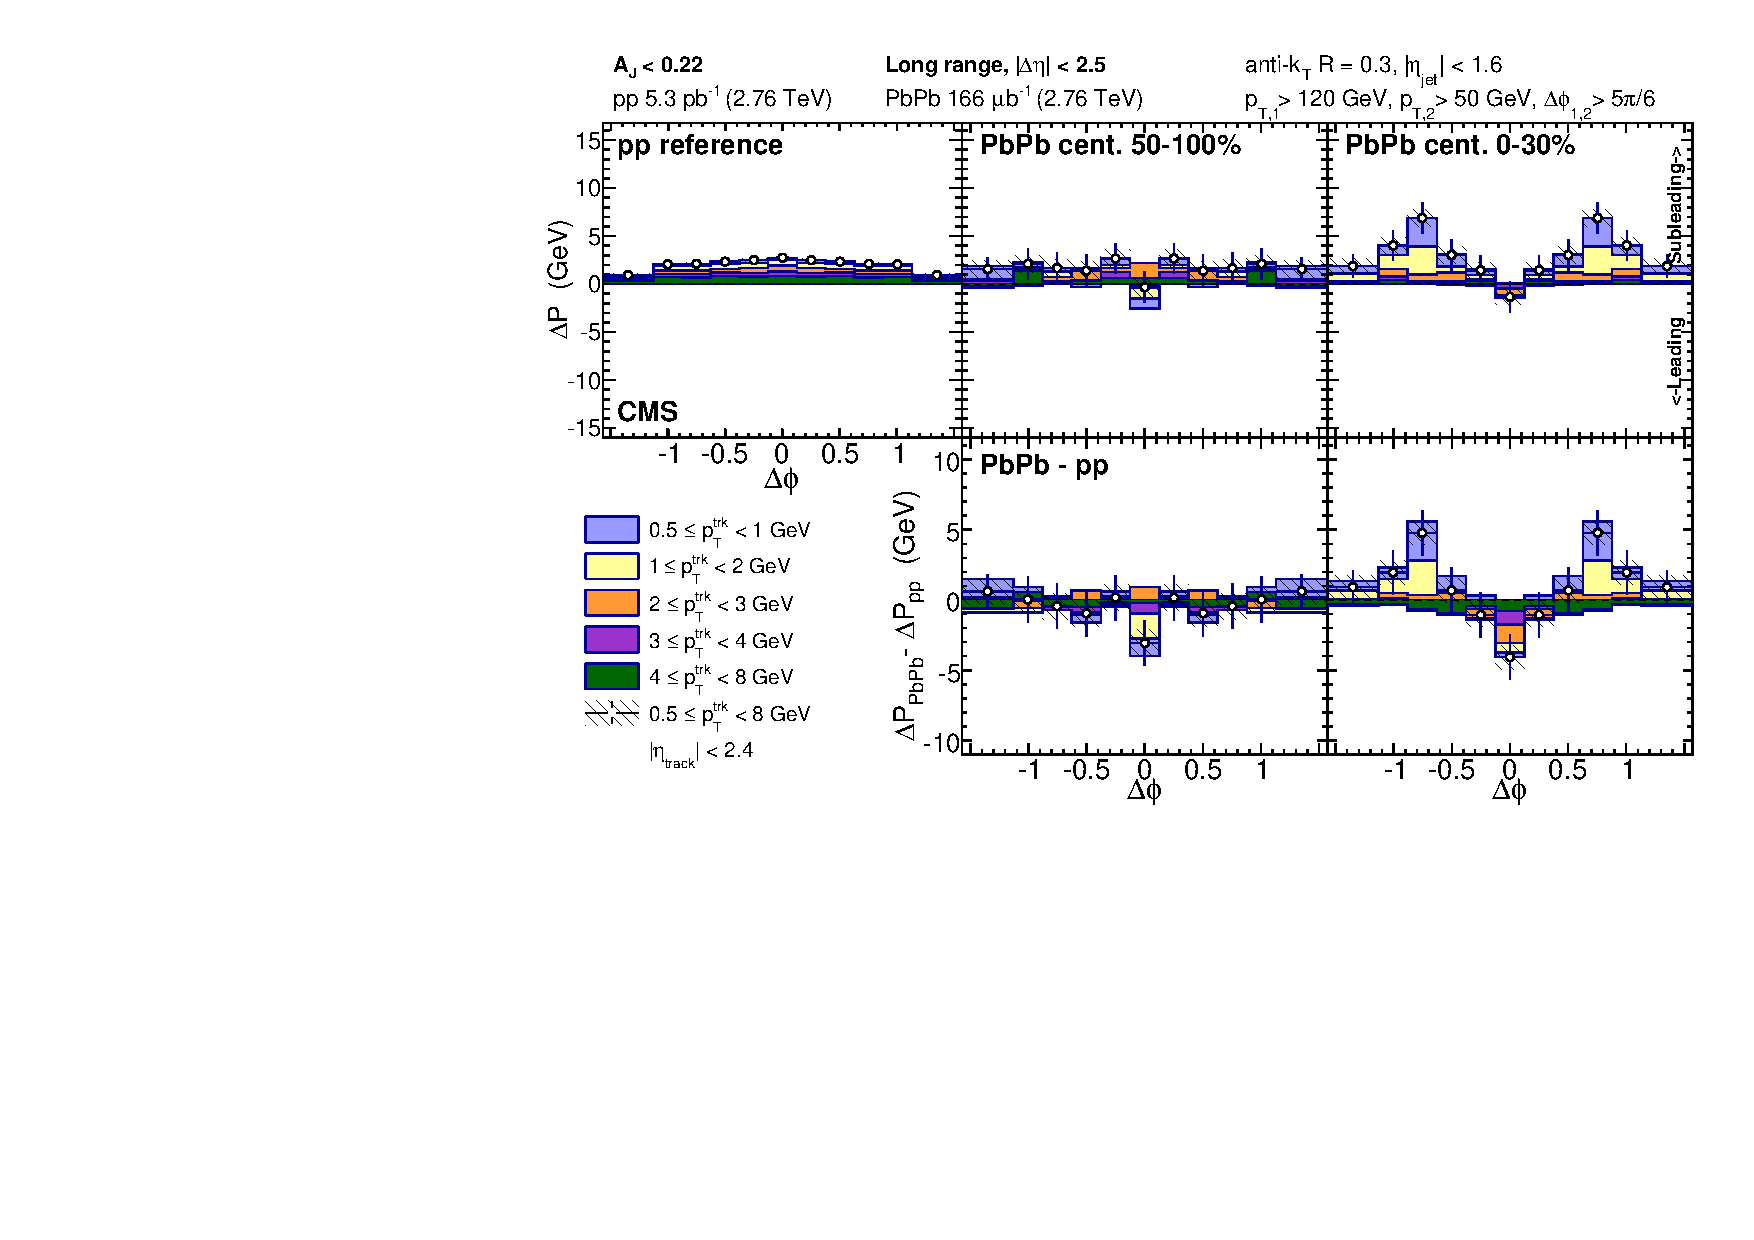
\includegraphics[width=0.99\textwidth]{figures/Results/Missing_pT_LongRange_Aj0_Aj22.pdf}
\caption[long-range subleading-to-leading momentum balance for balanced dijets]{Top row:  long-range distribution in $\protect\Delta\phi$ of excess tranverse momentum in the subleading relative to leading sides for balanced dijets with $A_{\rm J} < 0.22$.  Bottom row:  PbPb--pp difference in these $\protect\Delta\phi$ long-range momentum distributions.}
\label{fig:MpT_longrange_Aj0_Aj22} 
\end{center} 
\end{figure} 

\begin{figure}[hbt]
\begin{center} 
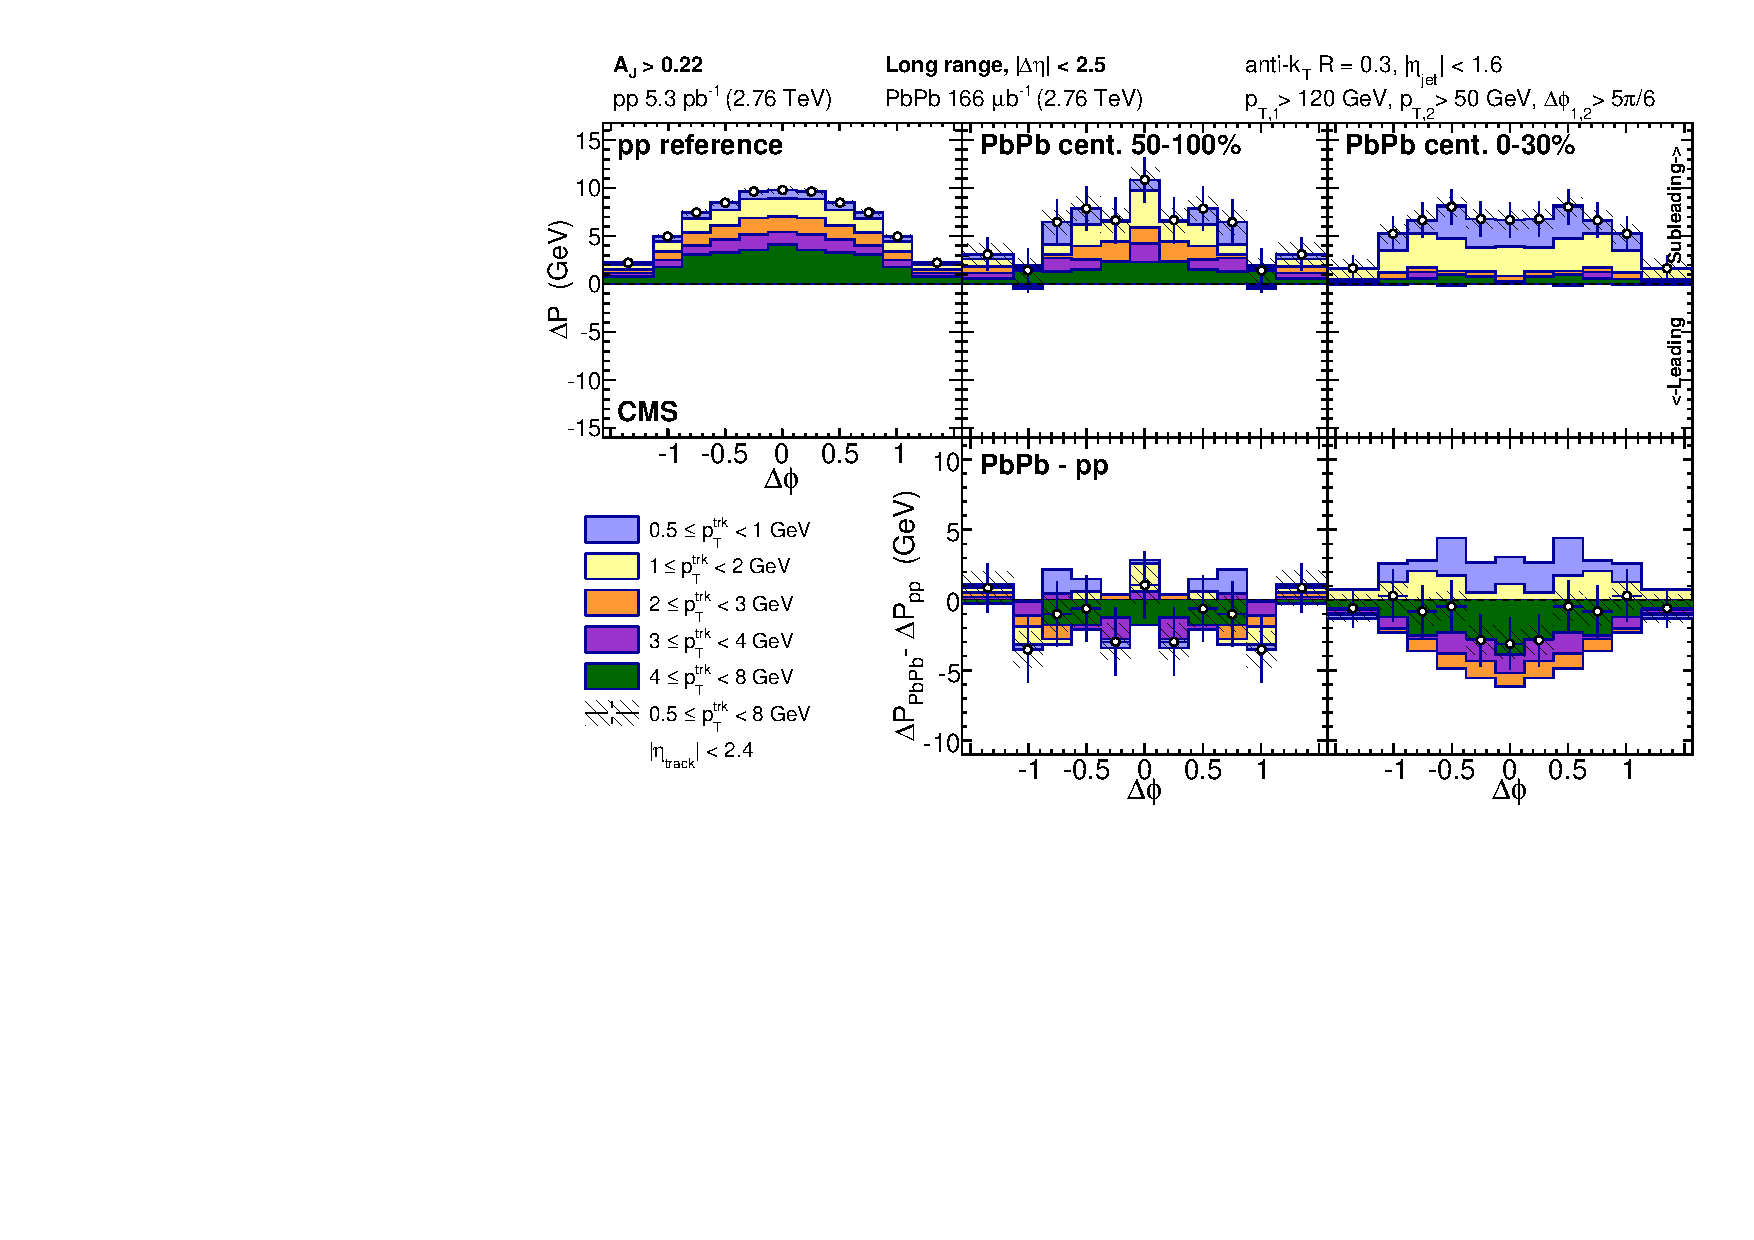
\includegraphics[width=0.99\textwidth]{figures/Results/Missing_pT_LongRange_Aj22_Aj75.pdf}
\caption[long-range subleading-to-leading momentum balance for unbalanced dijets]{Top row:  long-range distribution in $\protect\Delta\phi$ of excess tranverse momentum in the subleading relative to leading sides for balanced dijets with $A_{\rm J} > 0.22$.  Bottom row:  PbPb--pp difference in these $\protect\Delta\phi$ long-range momentum distributions.}
\label{fig:MpT_longrange_Aj22_Aj75} 
\end{center} 
\end{figure} 


\begin{figure}[h!]
\begin{center} 
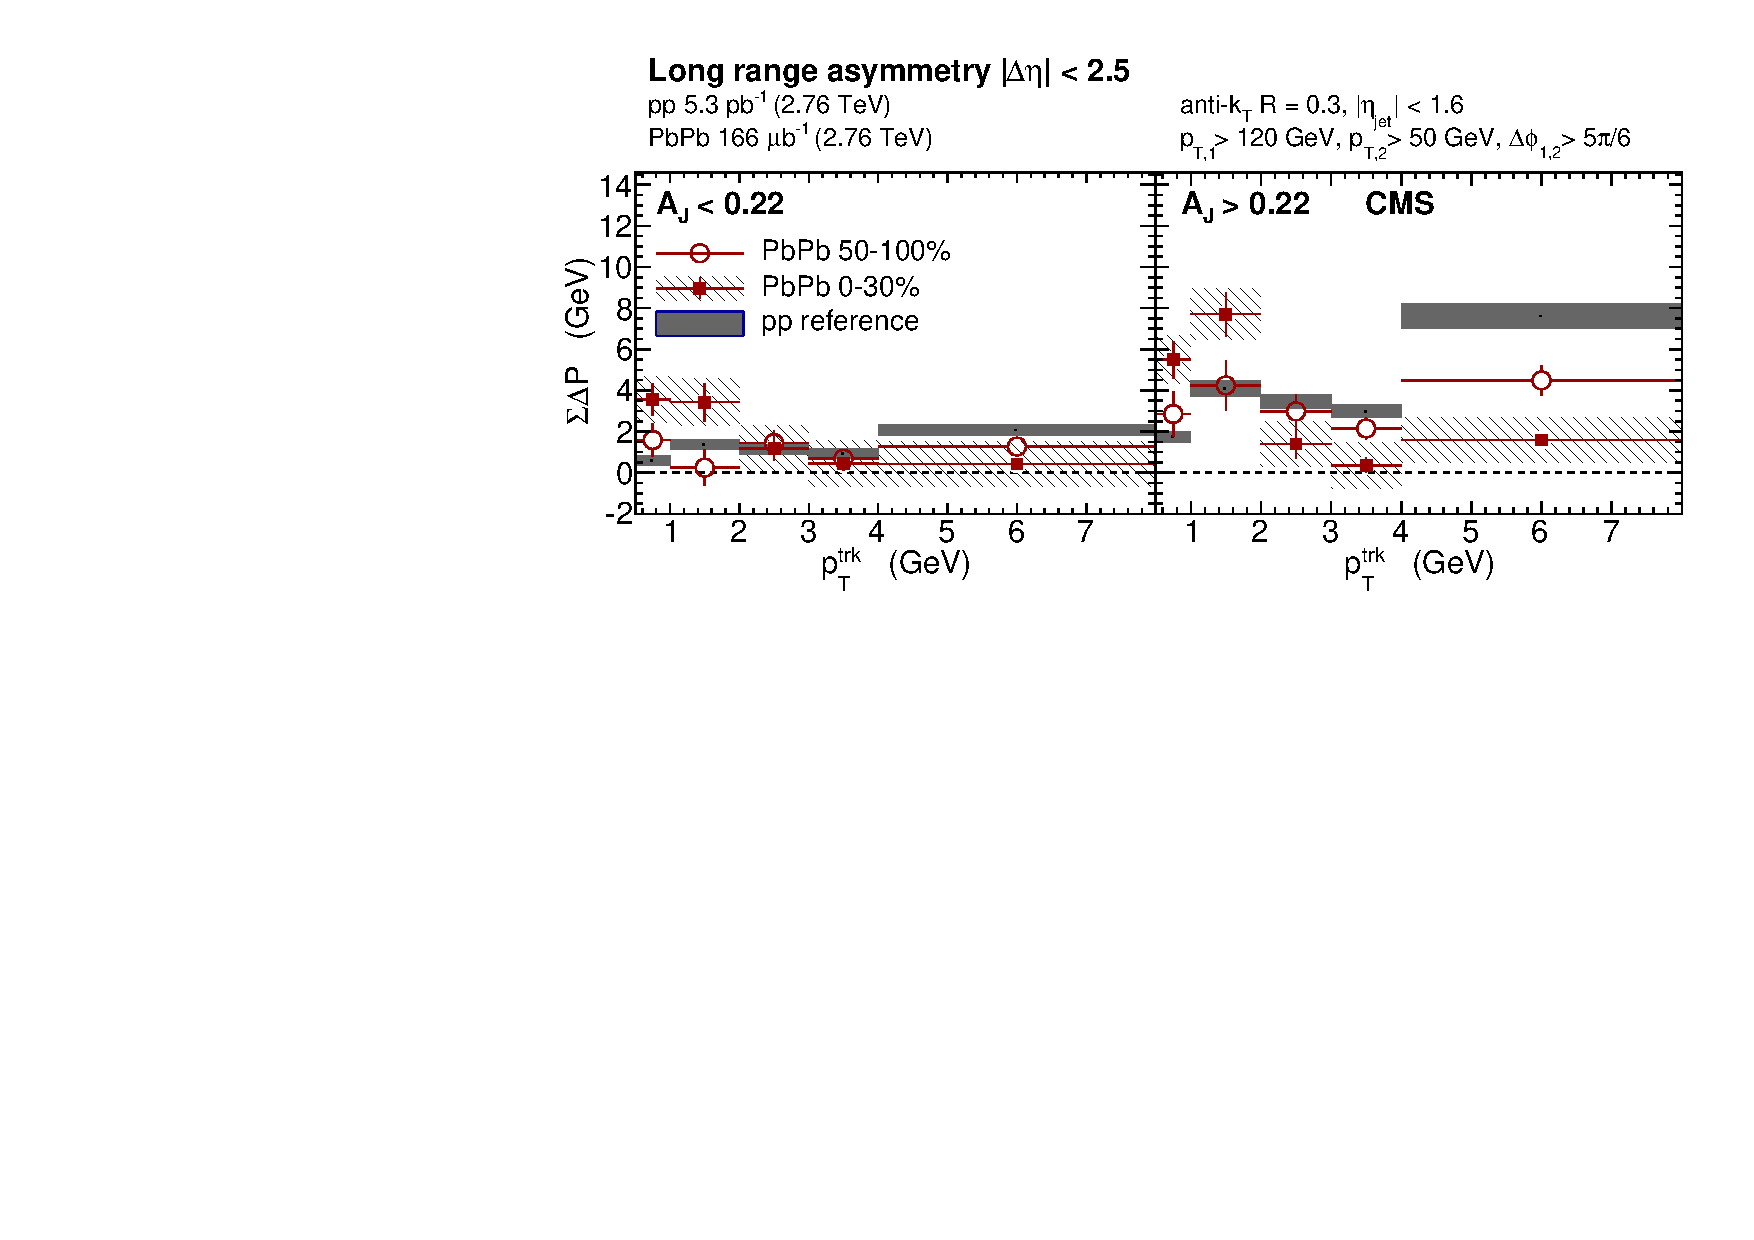
\includegraphics[width=0.99\textwidth]{figures/Results/Integral_Longrange.pdf}
\caption[Integrated transverse momentum in the long-range $\protect\Delta\phi$-correlated distribution as a function of track-$p_{\rm T}$]{Integrated transverse momentum in the long-range $\protect\Delta\phi$-correlated distribution as a function of track-$p_{\rm T}$ integrated over $|\Delta\phi| < \pi/2$  and $|\Delta\phi| < 2.5$ and for pp reference, peripheral PbPb and central PbPb data for balanced compared to unbalanced dijets.}
\label{fig:Integral_Longrange} 
\end{center} 
\end{figure} 


Finally, to show the relative conributions to overall hemisphere momentum balance from the leading and subleading jet peaks as well as from the long-range underlying event asymmetry, a summary of hemisphere-integrated excess (PbPb--pp) yield for balanced and unbalanced dijets in central PbPb collisions is shown in Fig.~\ref{fig:Integral_Summary} and Fig.~\ref{fig:Integral_Summary_Peripheral} for central and peripheral collisions respectively.  The top panels of Fig.~\ref{fig:Integral_Summary} present total PbPb minus pp differences in transvese momentum associated with the subleading jet (plotted positive) and leading jet (plotted negative).  Modifications to the distribution of tracks with $p_{\rm T}< 3$ GeV are evident for both the leading and subleading jet peaks, with a greater enhancement of low-$p_{\rm T}^{\rm trk}$ particles associated with the subleading jet.   These total jet peak modifications in central PbPb collisions are not significantly different in unbalanced versus balanced dijets.  The bottom panels of Fig.~\ref{fig:Integral_Summary} present these jet-peak modifications together with the long-range modifications evident in Fig.~\ref{fig:Integral_Longrange} to show the decomposed hemisphere-wide differences in associated transverse momentum in each $p_{\rm T}^{\rm trk}$ range.  Unlike the jet peak contributions, the long-range PbPb versus modifications differ outsie of uncertainties between balanced and unbalanced dijets:  here the depletion of high-$p_{\rm T}^{\rm trk}$ particles in unbalanced PbPb versus pp dijets corresponds to the reduced contribution from third jets (which are prominently evident in the long-range distribution for pp unbalanced dijet events) in central PbPb unbalanced dijet events.  Figure~\ref{fig:Integral_Summary_Peripheral} presents the same hemisphere-integrated PbPb minus pp excess information for peripheral collisions for comparison to the central results shown in Fig.~\ref{fig:Integral_Summary}.  Some possible small modifications are already evident in this 50-100\% centrality range, but these differences between peripheral PbPb and pp results are in most cases smaller than systematic uncertainties.


\begin{figure}[hbt]
\begin{center} 
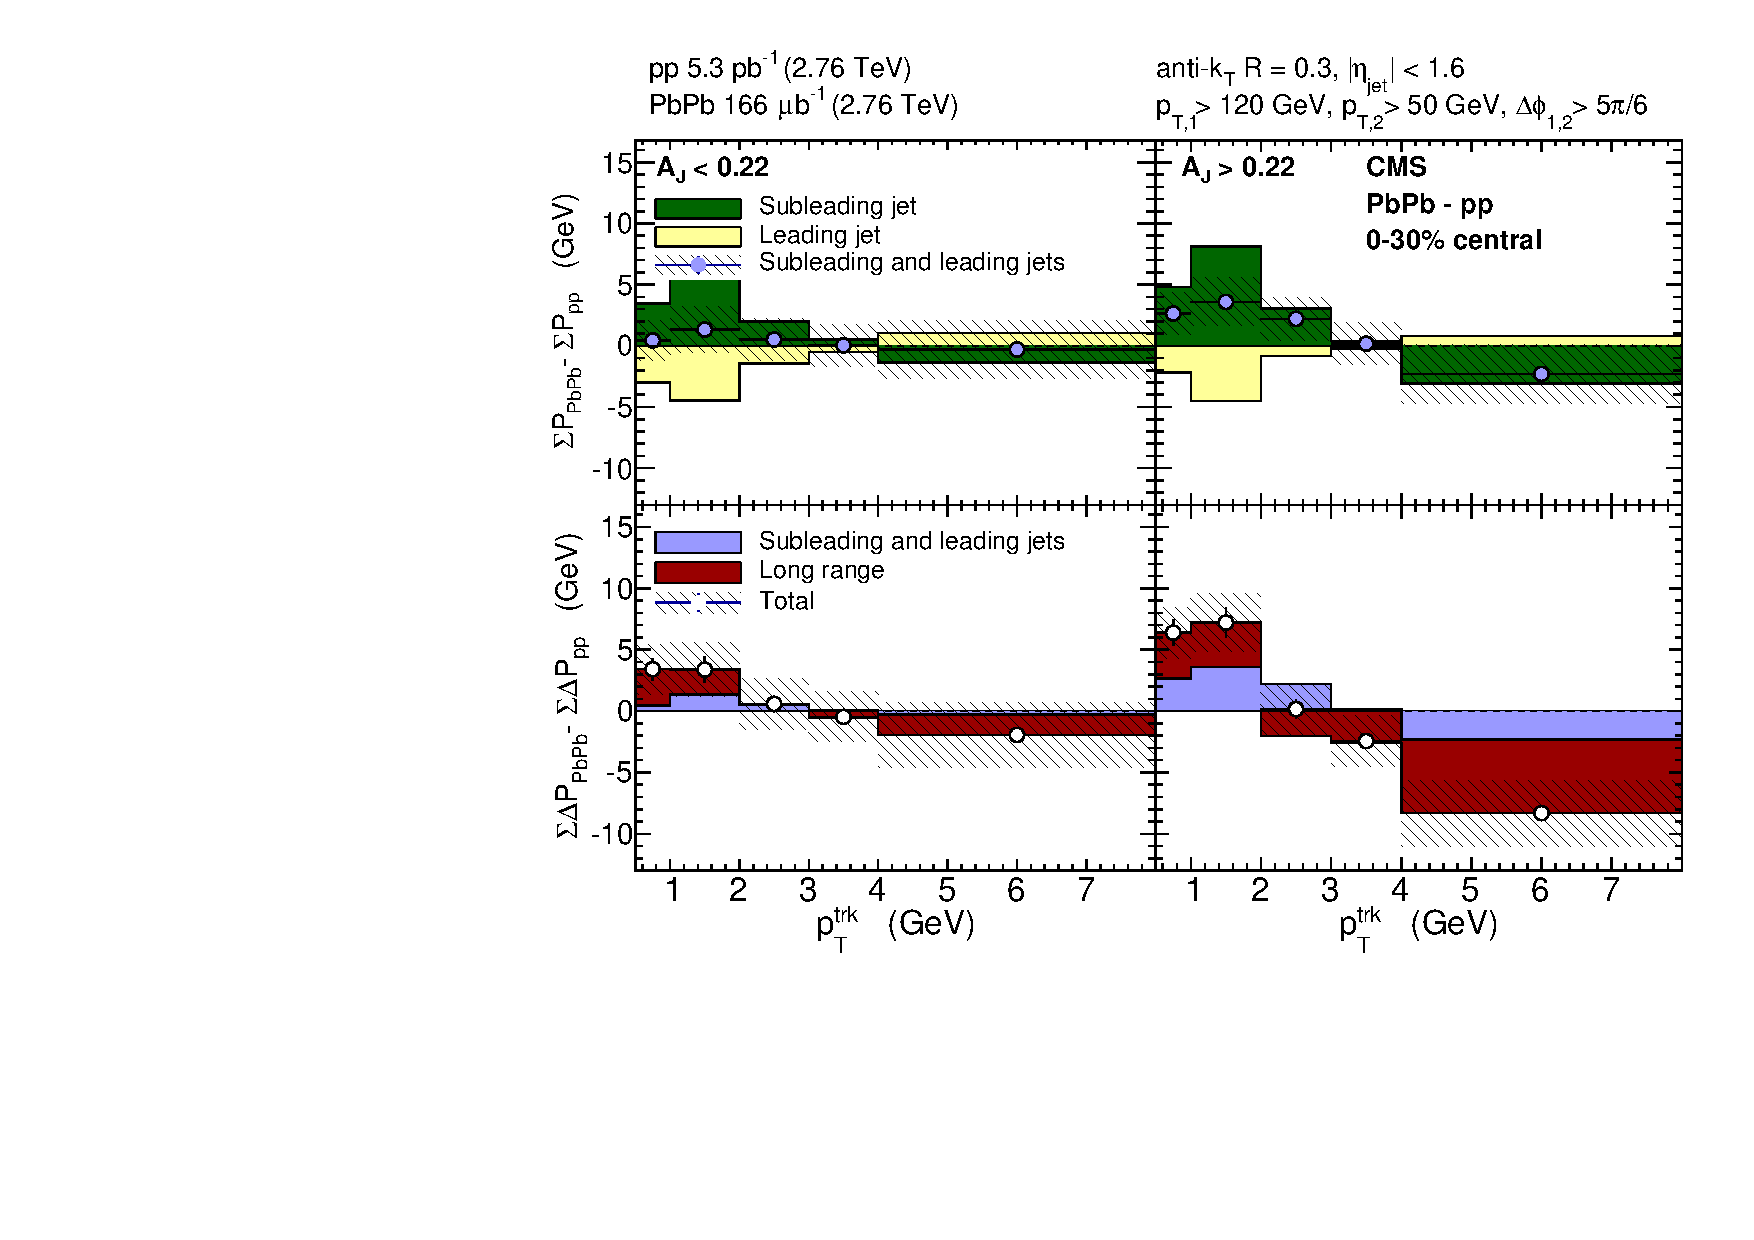
\includegraphics[width=0.99\textwidth]{figures/Results/Integral_PbPb_pp_Summary.pdf}
\caption[Relative contributions from jet peaks and long-range asymmetry to the double difference PbPb--pp, subleading--leading in total hemisphere transverse momentum for central collisions]{Modifications of jet-hadron correlated transverse momentum in central PbPb collisions with respect to pp reference, integrated $|\Delta\phi| < \pi/2$, $|\Delta\phi| < 2.5$.  Top row:  subleading and leading jet peak PbPb--pp.  Bottom row:  relative contributions from jet peaks and long-range asymmetry to the double difference PbPb--pp, subleading--leading in total hemisphere transverse momentum. }
\label{fig:Integral_Summary} 
\end{center} 
\end{figure} 


\begin{figure}[hbt]
\begin{center} 
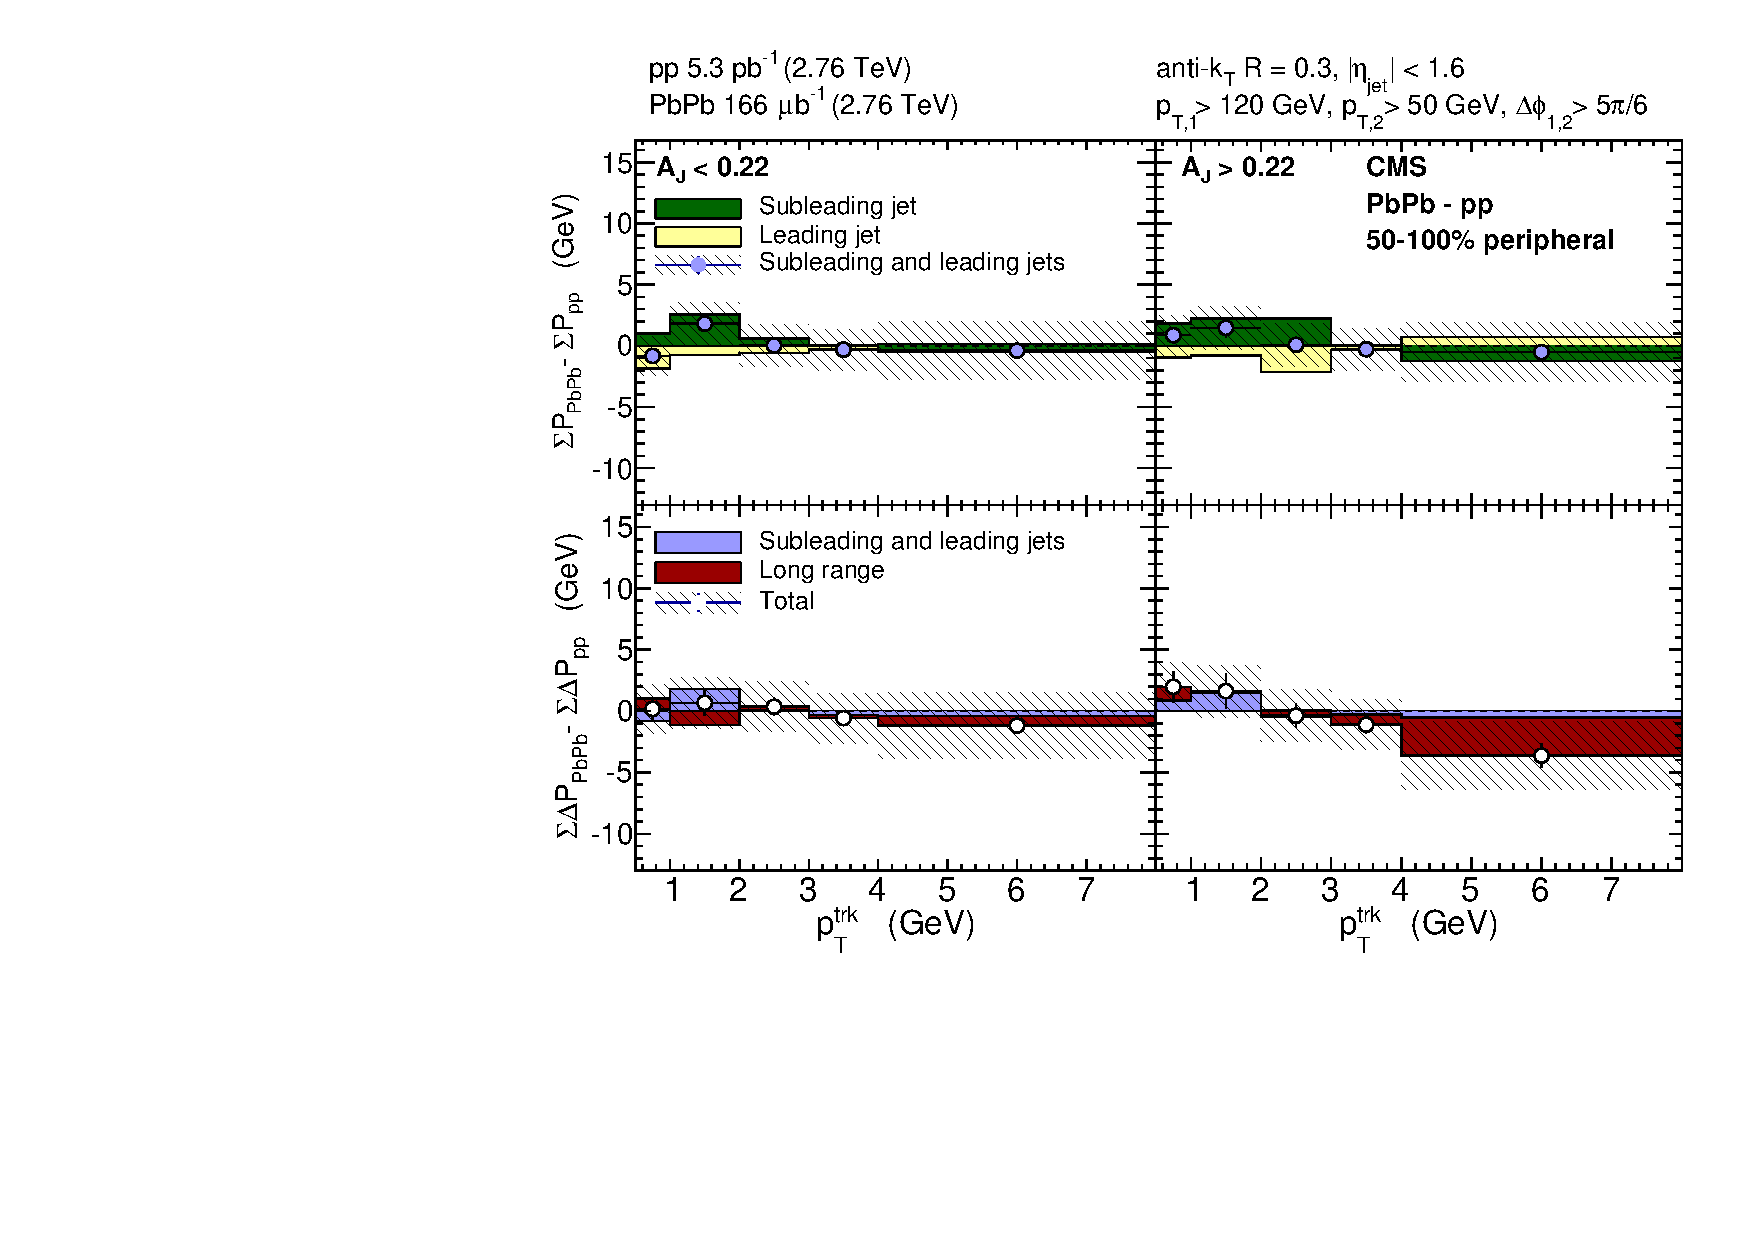
\includegraphics[width=0.99\textwidth]{figures/Results/Integral_PbPb_pp_Summary_Peripheral.pdf}
\caption[Relative contributions from jet peaks and long-range asymmetry to the double difference PbPb--pp, subleading--leading in total hemisphere transverse momentum for peripheral collisions]{Modifications of jet-hadron correlated transverse momentum in peripheral PbPb collisions with respect to pp reference, integrated $|\Delta\phi| < \pi/2$, $|\Delta\phi| < 2.5$.  Top row:  subleading and leading jet peak PbPb--pp.  Bottom row:  relative contributions from jet peaks and long-range asymmetry to the double difference PbPb--pp, subleading--leading in total hemisphere transverse momentum. }
\label{fig:Integral_Summary_Peripheral} 
\end{center} 
\end{figure} 


The decomposition of integrated jet peak and long-range correlated $p_{\rm T}^{\rm trk}$ shown in Fig.~\ref{fig:Integral_Summary} and Fig.~\ref{fig:Integral_Summary_Peripheral} clarify the relationship between the jet peak correlation studies presented in this analysis and the missing-$p_{\rm T}$ measurements presented in Ref.~\cite{HIN_2014_010}:  as shown through this detailed decomposition, comparing hemisphere distributions as a whole include contributions from the subleading and leading jet peaks studied in correlation studies, but also a contribution from the underlying event.  In both PbPb and pp data, the underlying event partially cancels with hemisphere subtraction:  contributions from combinatoric background and even flow harmonics ($V_{2}$ etc.) will cancel, while contributions from 3rd jets and and odd flow harmonics ($V_{1}$, $V_{3}$ etc.) will not.  As we have seen, in pp the non-cancelling underlying event is dominated by 3rd jets, especially in the unbalanced dijet selection in which their presence is kinematically required.  In PbPb (where the contribution from 3rd jet events is smaller), this underlying event has evident contributions from odd flow harmonics as well, reflecting coupling of jets to the event reaction plane.  

\clearpage


\subsection{Theory implications of these results}


https://arxiv.org/abs/1707.01539

